\documentclass[a4paper,12pt,twoside]{report}
% \documentclass[a4paper,12pt,twoside]{book}
\pagestyle{headings}
\usepackage[utf8]{inputenc}
\usepackage{filecontents}
\usepackage[many]{tcolorbox}
\usepackage{graphicx}
\usepackage{harpoon}
%\usepackage{apacite} 
\usepackage{xcolor}
\usepackage{latexsym}
\usepackage{amssymb}
\usepackage{amsmath}
\usepackage{mdframed}
%\usepackage[authoryear]{natbib}
\usepackage{hyperref, url}
\usepackage[show]{ed}
\usepackage{subfigure}
\usepackage[ntheorem]{empheq} 
\usepackage{amsthm, amssymb, amsfonts, latexsym}
% \usepackage{pst-all}

\usepackage{enumitem}
\usepackage{multirow}
\usepackage{longtable}
\usepackage[export]{adjustbox}
% $f\arrowvert_A$ To restrict functions

\setlength{\parskip}{1.7em}
\setlength{\parindent}{0em}


%\setlength{\baselineskip}{20pt}

\setlength{\textwidth}{429.75499pt}
\setlength{\textheight}{643.20255pt}
\setlength{\oddsidemargin}{5 mm}
\setlength{\evensidemargin}{5 mm}
\setlength{\topmargin}{0 mm}
\setlength{\headsep}{0 mm}
\setlength{\headheight}{0 mm}


\usepackage{pst-node}

\newcommand{\citealtt}[1]{\citeauthor{#1},\citeyear{#1}}
\newcommand{\myycite}[1]{\citep{#1}}

\mathchardef\mhyphen="2D

%\newcommand{\cev}[1]{\reflectbox{\ensuremath{\vec{\reflectbox{\ensuremath{#1}}}}}}


\usepackage{pst-node,graphicx,pst-blur}
%\uspackage{auto-pst-pdf}
%\usepackage{tikz-cd} 



\makeatletter
\DeclareRobustCommand{\cev}[1]{%
  \mathpalette\do@cev{#1}%
}
\newcommand{\do@cev}[2]{%
  \fix@cev{#1}{+}%
  \reflectbox{$\m@th#1\vec{\reflectbox{$\fix@cev{#1}{-}\m@th#1#2\fix@cev{#1}{+}$}}$}%
  \fix@cev{#1}{-}%
}
\newcommand{\fix@cev}[2]{%
  \ifx#1\displaystyle
    \mkern#20mu
  \else
    \ifx#1\textstyle
      \mkern#20mu
    \else
      \ifx#1\scriptstyle
        \mkern#26mu
      \else
        \mkern#26mu
      \fi
    \fi
  \fi
}

\makeatother

\newcommand{\xcm}{\epsfxsize=3.1cm}
\newcommand{\fig}[1]{\epsfbox}
% \newcommand{\bp}{\begin{minipage}{3.1cm}}
% \newcommand{\ep}{\end{minipage}}



\newtheorem{Definition}{Definition}[]
%\newmdtheoremenv{Theorem}{Theorem}[]
\newtheorem{Theorem}{Theorem}[]
\newtheorem{Lemma}{Lemma}[]
\newtheorem{Proposition}{Proposition}[]
\newtheorem{Corollary}{Corollary}[]
\newtheorem{Remark}{Remark}[]
\newtheorem{Example}{Example}[]


%Shortcut symbols
\newcommand{\Ftheta}{\ensuremath{F_\theta}}


\makeatletter 
\renewcommand{\thefigure}{\@arabic\c@figure}
\makeatother
\usepackage{xr}


%%%% PNAS GRAPHICS SETUP- FROM THE PNAS STYLE LATEX FILE
\RequirePackage{graphicx,xcolor}
\RequirePackage{colortbl}
\RequirePackage{booktabs}
\RequirePackage{algorithm}
\RequirePackage[noend]{algpseudocode}
\RequirePackage{changepage}
\RequirePackage[twoside,%
				letterpaper,includeheadfoot,%
				layoutsize={8.125in,10.875in},%
                layouthoffset=0.1875in,%
                layoutvoffset=0.0625in,%
                left=38.5pt,%
                right=43pt,%
                top=43pt,% 10pt provided by headsep
                bottom=32pt,%
                headheight=0pt,% No Header
                headsep=30pt,%
                footskip=25pt,
                marginparwidth=38pt]{geometry}
\RequirePackage[labelfont={bf,sf},%
                labelsep=period,%
                figurename=Fig. ]{caption}
\setlength{\columnsep}{13.5pt} % Distance between the two columns of text
\setlength{\parindent}{12pt} % Paragraph indent

%% Figure caption style
\DeclareCaptionFormat{pnasformat}{\normalfont\sffamily\fontsize{7}{9}\selectfont#1#2#3}
\captionsetup*{format=pnasformat}

%%% GREYBOX AROUND FIG
\definecolor{lightgray}{gray}{0.95}
\newcommand\greybox[1]{%
  \vskip\baselineskip%
  \par\noindent\colorbox{lightgray}{%
    \begin{minipage}{\textwidth}#1\end{minipage}%
  }%
  \vskip\baselineskip%
}

\newtcolorbox{paperbox}[1][]{
    enhanced,
    colback=white,
    boxrule=0pt,
    boxsep=0pt,
    arc=0mm,
    width=0.8\linewidth,
    fuzzy shadow={0mm}{-4pt}{-4pt}{1mm}{black!30!white},
    #1
}


% \externaldocument{Supp_Koopman-0808}
\begin{document}



\title{Data-Driven Modelling \& \\ Forecasting of Chaotic Systems}



\author{B.L. Nortier} 
\date{January, 2022}
\date{}
\maketitle


\begin{abstract}
  Collecting measurements from underlying artificial, natural, and physical systems through observables to realise a dynamical model with greater descriptive power is a well-established practice. Physical systems can often be modelled by instance with differential equations derived from the laws of physics, if we knew the laws.  However, we often do not fully understand the many complexities of the more intricate systems we interact with on a daily basis.
  In this project we start with the hypothesis that an discrete-time dynamical systems, particularly those which are chaotic generates the data. The general learning problem is then formulated and a well-known approach to the problem, alongside its practical limitations are considered.
  We then introduce the notion of driven dynamical systems and establish the theoretical existence of dynamical systems possessing certain properties that guarantee them to be topologically conjugate ('dynamically equivalent') to the dynamics of the underlying system from which measurements were taken. The methodology is practically implemented by making use of a recurrent neural network and using deep learning methods to train on the recurrent neural network states to show that we may obtain long-term consistent predictions for simple physical systems such as the double pendulum as well as a few other attractors exhibiting chaotic behaviour. The machine learning algorithms for modelling the double pendulum thus far have not been successful when it exhibits chaos. 


  \end{abstract}

  \tableofcontents

\chapter{Introduction}\label{ch1}

Experimenting on biological, physical, and artificial systems in order to generate a more informative dynamical model is a well-established practice in modern science. Traditional methods for modelling physical systems are based on laws of physics that are based either on empirical relationships or on intuition. For systems that evolve with time, physical laws yield mathematical equations that govern how the quantities evolve with time. However our world around is, for the most part, much more complex than that which can be distilled into elegant equations. We do not fully understand many of the more complex systems, nor do they even provide us with a good physical intuition of the underlying principles governing the dynamics. 
To complicate this - the underlying systems we observe often display sensitive dependence on initial conditions; despite having highly similar initial conditions, differing orbits diverge quickly and to such an extent that it becomes seemingly impossible to retrace their steps back to the original conditions. Even the presence of usually 'negligible' computational noise or measurement error renders long-term point-wise prediction infeasible. 
There are many difficulties that one encounters while modelling such systems:
\vspace{-8mm}
\begin{enumerate}[noitemsep, label=\roman*.]
  \item One may not have access to the complete states of the systems
  \item The actual system may be described by functions that behave wildly in the sense their graphs have a wild oscillatory behaviour, i.e., they have a large functional complexity.    
\end{enumerate}


Models derived primarily from data can be classified into three categories: 
\vspace{-8mm}
\begin{enumerate}[noitemsep, label=\roman*.]
  \item  Interpretable models (i.e., they establish relationships between internal physical mechanisms), 
  \item Partially interpretable models capturing some modes of the dynamics, 
  \item Non-Interpretable models, defined as such mainly due to the fact that they are defined on a different phase space that is usually high-dimensional. 
\end{enumerate}

Examples in the literature attempting to forecast data from such systems have tried a number of different approaches with differing degrees of success. 
When we have complete access to states of the system, an ordinary differential equation can be obtained from data (\cite{brunton2016discovering, champion2019data} and \cite{small2002modeling,xu2006modeling}) wherein one could approximate the vector field by a library of functions to obtain interpretable models. 


Recent partially interpretable models available in the literature have been based on the Koopman operator (e.g.,\cite{koopman1932dynamical,budivsic2012applied}) to  employ observables mapping the data onto a higher-dimensional space. This then makes the dynamics in the higher-dimensional space more amenable for approximation by a linear transformation. Such methods, obviously, do not guarantee an exact reconstructions for nonlinear models, and in practice provide poor long-term consistency for a large class of systems. \textbf{(Citation)}

The non-interpretable models include the delay embedding and the machine learning algorithms. One could learn a system conjugate to the underlying system by applying the Takens delay embedding \cite{takens1981detecting} when one has ``good" observations from the system; this learnt system could then be used for forecast the observed data.  Takens delay embedding theorem \cite{takens1981detecting} and its various generalisations (e.g., \cite{sauer1991embedology, stark1999delay, gutman2018embedding}) establishes the learnability of a system constructed by concatenating sufficiently large previous time-series observations of a dynamical system into a vector (called delay coordinates). This then establishes the existence of a map on the space of delay coordinates equivalent (or topologically conjugate) to the underlying map from which the observed time-series was first obtained. Although topological conjugacy guarantees an alternate representation of the underlying system, the quality of this representation still depends on numerous parameters, making the comprehension of the dynamics rather unreliable (e.g., \cite{principe1992prediction}). One reason for this fragility is that the embedded attractor in the reconstruction space not always an attractor of the map that is learnt in the reconstruction space, despite  unquestionably being an invariant set. When the embedded object is not explicitly known to be an attractor (as explained in Chapter \ref{ch3}) it can cause predictions to fail.


Practically, the application of Takens embedding involves learning a map through some technique and consequently one wishes that these would have low functional complexity\cite{manjunath2021universal}, i.e., functions with fewer oscillatory graphs. Pure machine learning methodology that processes temporal information (like the echo state networks (Citations to echo state networks)) by mapping data onto a higher dimensional space for further processing. Although they perform  well on forecasting some dynamical systems, they fail completely on others (Citations here) as there is often no guarantee that the right function was learnt during training.

This thesis deals with the implementation and analysis of non-interpretable models that can guarantee exact reconstruction. The project work concerns the study and implementation of a method (\cite{manjunath2021universal}) that incorporates learning a function by mapping the data on to a higher dimensional space using what is called a driven dynamical system (See Chapter 4). With a clear understanding of how the data is mapped onto the higher dimensional space, the method then permits the learning of a dynamical system topologically conjugate to that of the underlying system. Instead of linear regression as in the training of echo state networks, deep learning methods are employed to learn the correct function. With slight modifications to the implementation in the paper (with Adriaan), we show that one can construct accurate non-interpretable models with the ability to reconstruct attractors from more hard-to-forecast systems like the double pendulum. (The forecasting of the time-series from a double pendulum has not been reported before.) Moreover, we also demonstrate that long-term statistical consistency is preserved.

\emph{By solidifying the mathematical underpinnings of our theory, we hope to guarantee the ability to construct models with predictive power ranging from molecular biology to neuroscience. in the near future. (We can modify this sentence when the report is completed.)}

The more intricate details of proofs are referred to where relevant throughout. This report is organised as follows: 
\newline In Chapter~\ref{ch2}, we recall the definition of a discrete-time dynamical system, how a discrete-system arises from a flow of an ODE and then proceed to define the inverse-limit space and topological conjugacy of autonomous systems. 
\newline In Chapter~\ref{ch3}, we introduce the problem of forecasting dynamical systems, state the Takens delay embedding theorem and discuss various issues faced while forecasting. 
\newline In Chapter~\ref{ch4}, a driven dynamical system is defined and discuss the properties of a specific class of driven dynamical systems that we make use of in this thesis/report/paper. 
\newline Finally in Chapter~\ref{ch5} we show the implementation of these forecasting methods, and conclusions are provided in Chapter~\ref{ch6}.


\chapter{Discrete-time Dynamical Systems}\label{ch2}

In this chapter, we provide a brief description of what a discrete-time dynamical system is and what it means for it to exhibit chaos. We refer to \cite{devaney2018introduction, de2013elements} for more details. 

At its most elementary level, a dynamical system is just something that evolves deterministically through time. In the context of this thesis, deterministic refers to the fact that a system evolves according to specified rules rather than based on random events. 
Dynamical systems arise in a variety of situations. A continuous-time dynamical system describes the states for all values of the time. Specifically, if the motion of a pendulum in which the quantities such as the angular position and angular momentum are known at all times, then it is a continuous-time dynamical system. The equations of the dynamical system can take the form of one or more ordinary differential equations that determine the relevant quantities at any future time if we know the initial location and momentum. 
In ecology, discrete-time dynamical systems are widely used to model population growth. The model in this case is a function calculating the following generation's population given the population of the previous generation. If we know the starting population, we may once again calculate the population at any time in the future. 

Formally, a function $T: U \to U$, where $U$ is some set is  a \emph{discrete-time dynamical system} and its iterates $\{u,Tu,T^2u,\ldots\}$, where $T^n$ denotes the $n$-fold composition of $T$ with itself, describe the evolution of an initial condition $u\in U$ (Note that we frequently drop the brackets and denote $T(u)$ by $Tu$ so as to simplify notations).  





Continuous-time dynamical systems modelled using ordinary differential equations can give rise to discrete-time dynamical systems. To see this, consider a differential equation $\dot{x} = f(x)$, $f: \mathbb{R}^n \to \mathbb{R}^n$, $n\in\mathbb{N}$ given to have a unique solution passing through 
each point $x\in\mathbb{R}^{n}$, call it $x(t)$ where $x(0)=x_0$. 

\begin{Definition}
  [\bf Flow of an Equation] \label{Dfn_Flow}\rm
  The flow of the equation  $\dot{x} = f(x)$  is defined to be a mapping $\varphi: \mathbb{R}^n \times \mathbb{R} \to \mathbb{R}$ where $\varphi(x_0,t)= x(t)$ for the solution $x(t)$ with $x(0)=x_0$ 
\end{Definition}

By fixing $t=K \in (0,\infty)$, we can define the \emph{time-$K$ map} as  $T(x):= \varphi(x_0,K)$, and it is easily verified that $T\circ T(x_0) = \varphi(x_0,2K)$. In general the $m^{\mbox{th}}$ iterate of $x_0$ under $T$ would be the value of the solution of the ODE evaluated at time $mK$ with the initial condition $x_0$, i.e. $\varphi(x_0, mK)$. 
Thus ordinary differential equations give rise to a discrete-time dynamical system by sampling the value of the solution $x(t)$ at time intervals $K$ units apart. 


A numerical discretization of a differential equation can also give rise to a discrete-time dynamical system. For instance, Euler's method approximates $\dot{x}(t)$ by $(x(t+h)-x(t))/h$; if $h$ is fixed throughout, the solution of a differential equation $\dot{x}=f(x)$ 
can be approximated at the time instant $t+(m+1)h$ by iterating the equation 
\begin{equation}
  x(t+(m+1)h) = x(t+mh) + h f(x(t+mh))
\end{equation}

Adopting more succinct notation by replacing $x(t+mh)$ with $u_m$, we rewrite the above equation as
\begin{equation}
u_{m+1} = u_m + hf(u_m)
\end{equation}
or in even simpler terms as the discrete-time dynamical system with map $T(u) = u + hf(u)$, where $T$, $u$ and $f$ are understood to be as above.


Of course, discrete-time dynamical systems need not always arise through a differential equation, and once again we may consider the field of ecology where discrete dynamical systems are often directly derived or assumed. \textbf{Citation}
There is a school of thought that advocates discrete-time dynamical systems to be more natural for modelling real-world observations than differential equations and we refer the interested reader to \cite{saber2010introduction}.


\section{Invariant Sets}

A core concept in the study of dynamical systems is that of invariance. 
\begin{Definition}
  [\bf Invariant Set]\label{Dfn_InvariantSet}\rm
  Given a discrete-time dynamical system $T: U \to U$, a subset $A \subset U$ is said to be an \emph{invariant set} if $T(A) =A$. 
\end{Definition}

We also define the orbit of a function $T$.
\begin{Definition}
  [\bf Orbit of $T$]\label{Dfn_Orbit}\rm
  The orbit of $T$ is to be defined the sequence $\bar{u} = \{u_n\}_{n\in \mathbb{Z}}$ obeying the update equation, $u_{n+1}=Tu_n$, $n \in \mathbb{Z}$. 
\end{Definition}

Two examples of invariant sets include a fixed point where $Tu=u$ for  $u\in U$, and a periodic orbit, i.e., a set of iterates $\{u,Tu, T^2u,\ldots,T^pu\}$, where $T^{p+1}u=u$ for some $p\in\mathbb{Z}$.  The entire space $U$ could be also be invariant.
Consider for example the space $U=[0,1]$, where $Tu=4u(1-u)$ and then $U$ is invariant (as every $u\in{U}$ can be written as $u = 4x(1-x)$ for some $x\in{U}$).

We may learn a great deal about the iterates of a dynamical system by considering the types of invariant sets of a discrete-time dynamical system.  For example, if $U=[0,1]$ has map $Tu= u/2$, then the only invariant set is $\{0\}$, and all orbits approach this invariant set as time flows in the forward direction. 
Indeed, if a some non-zero invariant set (call it $B$) exists, then there is  some $r\in(0,1]\cap{B}$. But $r\notin{T(B)}$ since any orbit with initial value $r$ will be a decreasing sequence. Moreover, every orbit of T will be decreasing and therefore approach the value $0$ as $n\rightarrow\infty$.

One may ask if every orbit approaches an invariant set? In general the answer is no, since for the dynamical system $T: \mathbb{R} \to \mathbb{R}$ defined by $Tu=2u$, any orbit that does not intersect the invariant set $\{0\}$, will not approach any invariant set. 

However,  when the space $U$ is compact, all orbits approach an invariant set. This is since the set of limit points of the orbit can be shown to be invariant \cite{de2013elements}. So, when $U$ is compact,  the $\omega$-limit set $\omega(u;T)$ of a point $u$ defined to the collection of limit points of the sequence $\{x,Tu,T^2u,\ldots\}$ is nonempty, and $\omega(u;T)$ is invariant. 

\begin{Example}
  For the map $Tu=u^2$ defined on $[0,1]$ all orbits lie in the invariant set $\{1\}$ or else would would approach the invariant set $\{0\}$. 
\end{Example}


Invariant sets have various properties. Invariant sets can be attracting or repelling depending on how orbits in its vicinity behave. 
Recall the examples $Tu =u/2$ and $Tu=2u$ defined on $\mathbb{R}$ (where $\{0\}$ ``attracts" orbits) or the example, $Tu=u^2$ defined on $[0,1]$ (where $\{1\}$ ``repels" orbits). We are interested in attractive invariant sets since they capture the long-term dynamics as time increases. 
In particular we are interested in those invariant sets named attractors.

\begin{Definition}
  [\bf Attractor]\label{Dfn_Attractor}\rm
  Let $T: U \to U$, where $U$  is a metric space with metric $d$. A compact subset $A \subset U$ is said to be an attractor if it satisfies the three conditions: 
  \vspace{-8mm}
  \begin{enumerate}
	\item $A$ is invariant. 
	\item $A$ is asymptotically stable, i.e., for every $\epsilon > 0$ and for all $u$ so that $d(u,A) < \epsilon$, we have $d(T^nu,A) \to 0$ as $n\to \infty$. 
	\item $A$ has Lyapunov stability, i.e., for every $\epsilon > 0$  there exists a $\delta(\epsilon) > 0$ so that $d(u,A) < \delta$ implies $d(T^nu,A) < \epsilon$ for all $n\ge 0$.  
\end{enumerate}
\end{Definition} 

Indeed in our previous examples, it can be verified that the system  $Tu=u/2$ defined on  $\mathbb{R}$ and $Tu=u^2$ defined on $[0,1]$  the singleton set $\{0\}$ is an attractor.  For the system,  $Tu=1-|2u-1|$ on $[0,1]$, one may easily verify that the only attractor is the entire space $[0,1]$. This is since between any two points $u< v$ in $[0,1]$, and for any $a,b$ so that $u\le a < b \le v$, we can find an $n$ so that $T^n(a,b)=[0,1]$ (as would be explained later in this chapter). 

A dynamical system can have several attractors, and may also be contained in another attractor. For the example, $Tu =u^2$ on $[0,1]$, both $\{0\}$ and $[0,1]$ are attractors. It is a known result that for dynamical systems on a compact space there always exists an attractor. 

The dynamics restricted to an invariant set can be complicated. For instance an invariant set could be just a single point or it could have an infinite set.    If the invariant set is infinite then there is a possibility of complicated dynamics, and a particular well-studied phenomenon of such complexity gives rise to what is called  chaotic behaviour, and has been studied in detail over the last fifty years.

% If the dynamics on the attractor are somewhat complicated in the sense that the attractor cannot be decomposed further, and if the attractor is infinite then there is a possibility of complicated dynamics, and a particular well-studied phenomenon of such complexity gives rise to what is called a chaotic behaviour. 

%If the dynamics on an attractor cannot be decomposed further and the attractor is itself also infinite, then there is a possibility of complicated dynamics, and a particular well-studied phenomenon of such complexity gives rise to what is called chaotic behaviour. 

\section{Chaos}

In the 1960s, a number of mathematicians and mathematically interested scientists independently discovered chaos in the mathematical sense. The meteorologist Edward Lorenz may have been the first to explain this phenomenon in his 1963 paper \cite{lorenz1963deterministic}. The notions of invariance, attractivity and chaos may also be described for continuous systems, and Lorenz's system comprised of a system of differential equations. The narrative of Lorenz's discovery of chaos, as well as the history of other forerunners in this subject, are fascinating. For those who are interested, we highly recommend James Gleick's book Chaos: The Making of a New Science \cite{gleick2008chaos}. It clearly illustrates these experiences, explains why chaos was such a startling and crucial mathematical and scientific discovery, and describes the underlying mathematical notions for non-specialists.

There are several intricately different definitions of chaos available in the literature \textbf{(Cite)}, with each of them indicating some aspect of complexity.
In practice, it is not possible to verify which definition or notion does the underlying dynamical system satisfies when only data is observed from it. We do, however, specifically recall the definition of chaos in the sense of Devaney \cite{devaney2018introduction,de2013elements} so as to understand some nuances behind the complexity. Devaney's definition of chaos has three requirements, with the first being the notion  of sensitive dependence on initial conditions. 

\begin{Definition}\rm
  [\bf {Sensitive Dependence on Initial Conditions}]\label{Dfn_SDIC}\rm
A dynamical system $T: U \to U$ is said to have sensitive dependence on initial conditions (SDIC) if there exists a $\delta > 0$ such that for every $u \in U$ and in every neighborhood of $u \in U$ there exists a $v\in{U}$ and an integer $N:=N{(u,v)}\in\mathbb{Z}$ such that $d(T^Nu,T^Nv)>\delta$. 	
\end{Definition}

It is important to acquire a sense of this definition as it can easily be misunderstood. It is common misconception to interpret SDIC as two close points ($u$ and $v$) that eventually become separated by a distance $\delta$ under iteration by $T$. But this is not true. To fully comprehend all the subtleties of the concept, one needs to discuss it more thoroughly by considering each sentence with care and attention, whereafter one may examine how they fit together to convey the concept of sensitive dependence. 

To this end, we make 3 remarks:
\vspace{-5mm}
\begin{enumerate}
  \item First, the $\delta>0$ in the definition of SDIC is independent of $u$. 
  \item Second, in every neighborhood of $u$, we may not necessarily find all points $v$ in the neighborhood distinct from $u$ that would separate from the forward iterates of $u$. 
  \item  Finally, $N$ depends upon $u$ and $v$ chosen, and their iterates may not separate for ever (i.e., for all $n>N$) and we allow their iterates to get arbitrarily close in the future. 
\end{enumerate}

To illustrate the concept of SDIC, we present two examples - one from Mathematics and the other from the field of Physics.

\begin{Example}
  The logistic map(LM), a recursion relation of the form $x_{n+1}=rx_n(1-x_n)$ where $x_n\in[0,1]$ and $r<4$ is of particular interest to us as it is classically used to illustrate the influence of chaos on a system \textbf{(Cite)}. Below are plotted the first 75 iterates of the LM for $r=3.7$ and $x_0=0.2$ with an adjustment of 0.001 in $x_0$ and $r$ respectively.

  \begin{figure}[ht]
    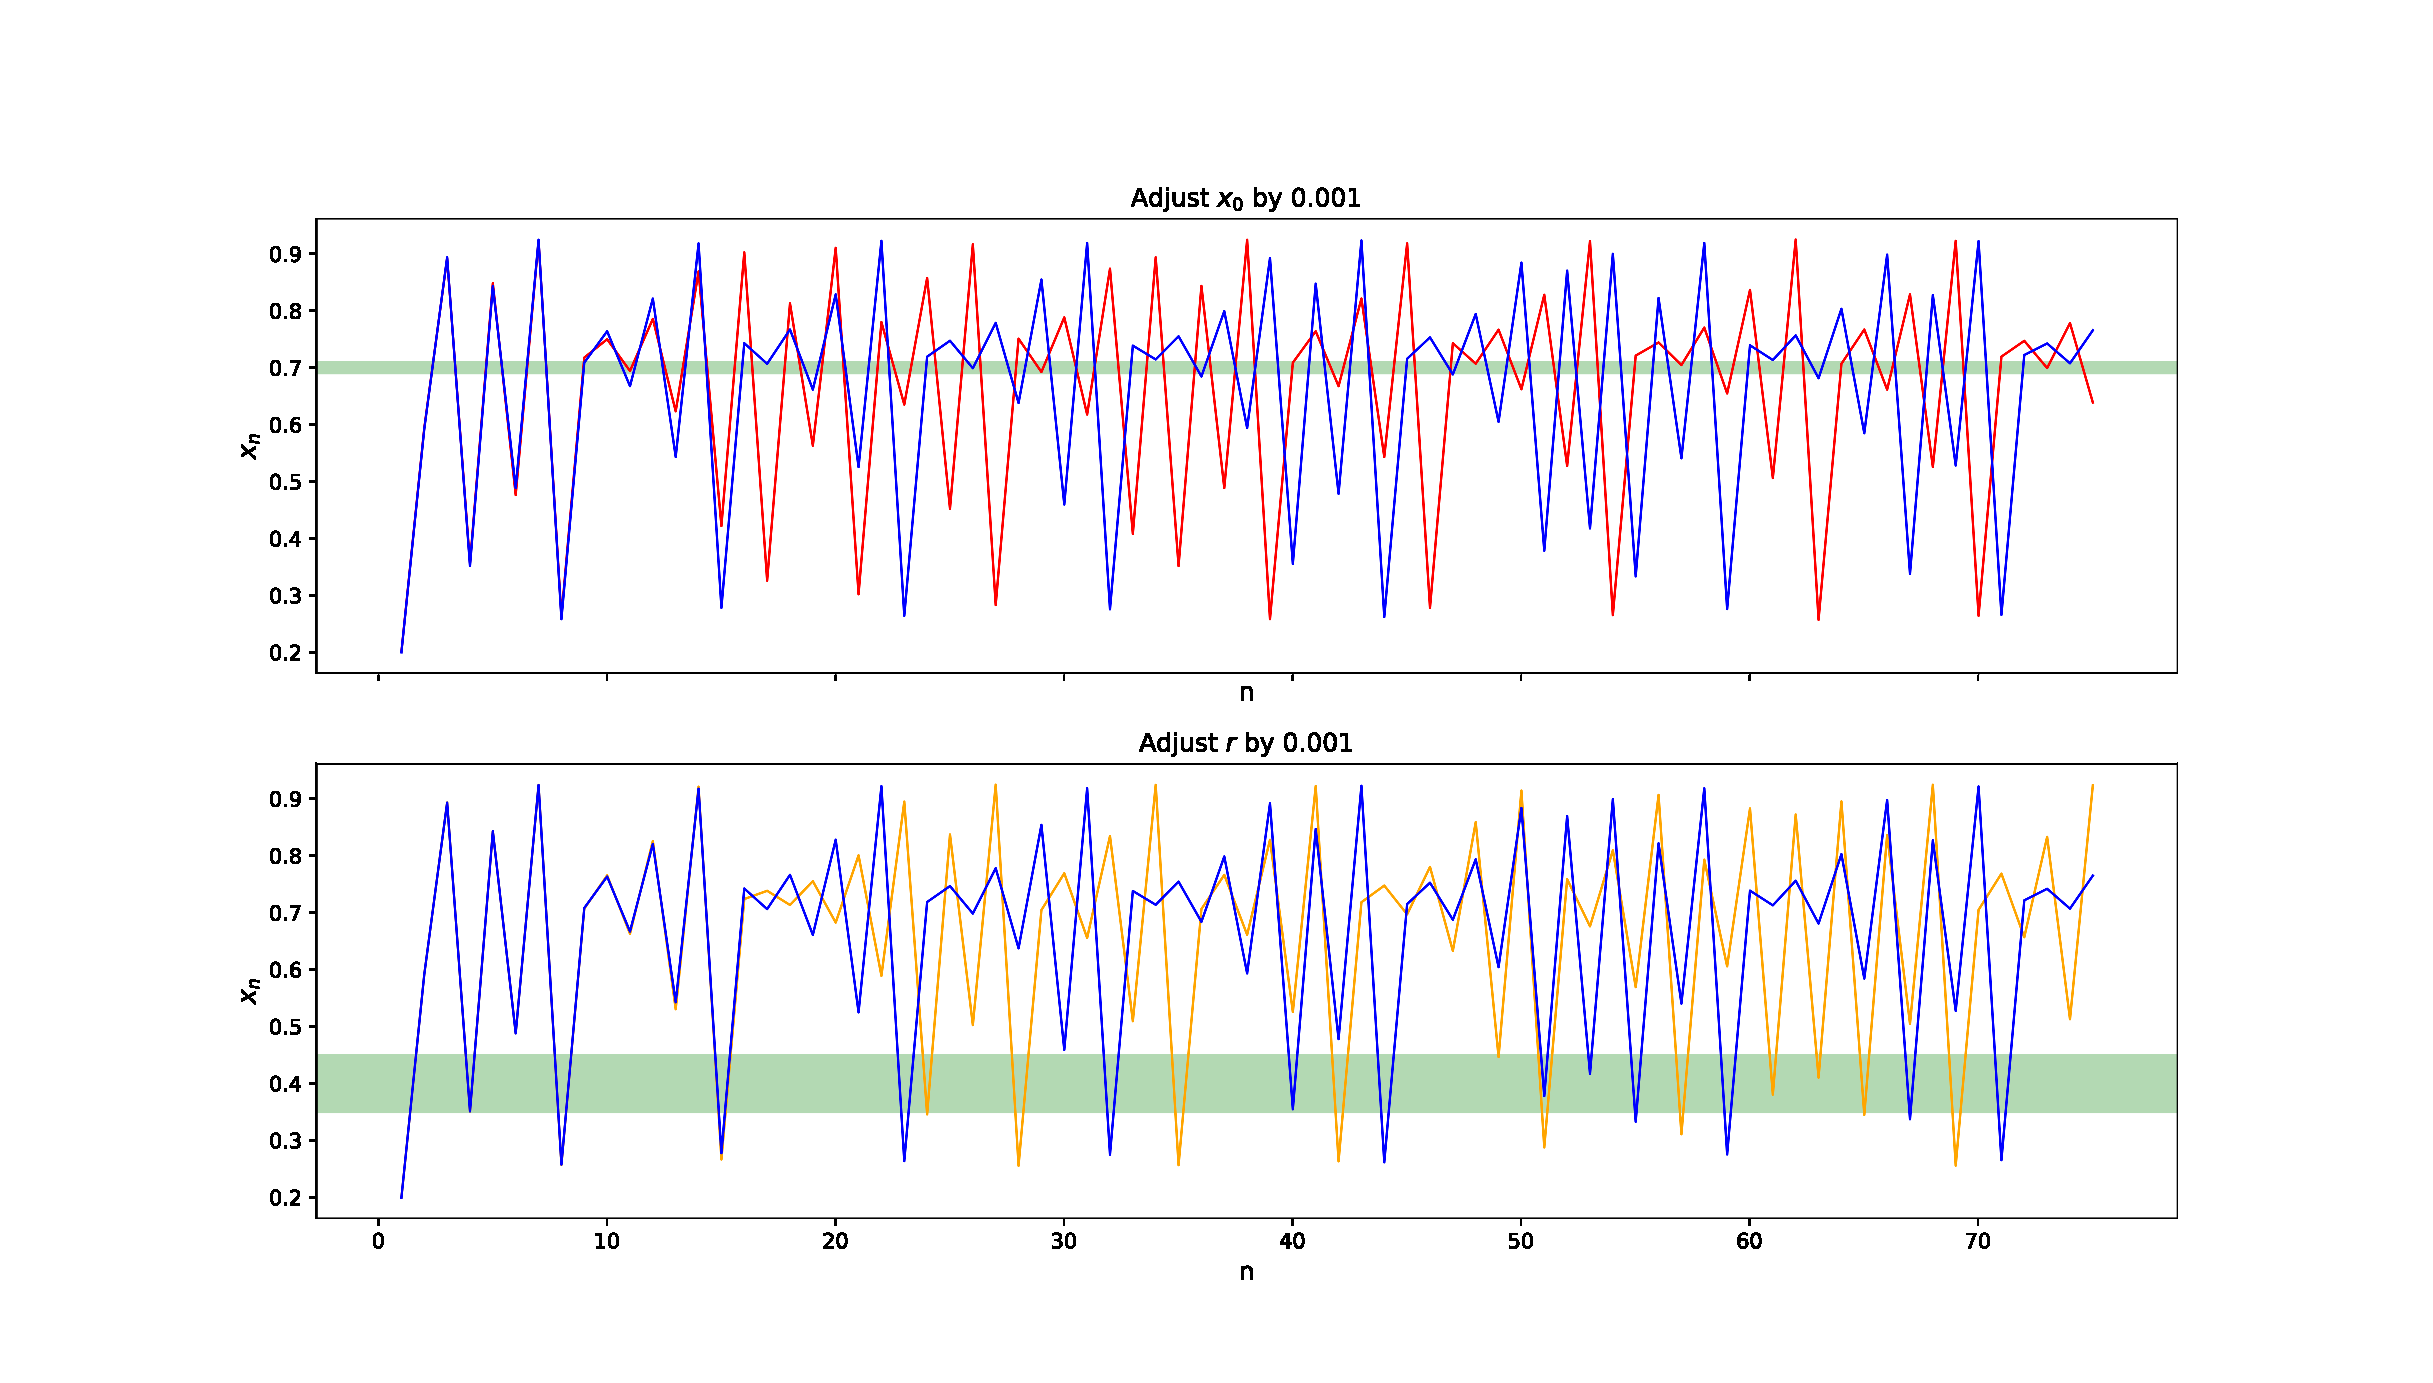
\includegraphics[scale=0.45]{_log_sdic.eps}
        \centering
        \label{fig:log_sdic}
        \captionof{figure}{Figure generated for Logistic Map for $r=3.7$, $x_0=0.2$ where each parameter is varied separately by 0.001.}
      \end{figure}
  
  For an intuitive sense of the fact that the LM exhibits SDIC, we draw two green neighbourhoods of diameters $\delta_1=0.1, \delta_2=0.02$ around the points $u_1=0.7, u_2=0.4$ respectively. It is easy to see that every neighbourhood around these two points will contain some $v_1, v_2\in[0,1]$ and natural number $N_1, N_2 \in\mathbb{N}$ respectively s.t. the distance $d(T^Nu_1,T^Nv)>\delta_1=0.02$ and $d(T^Nu_2,T^Nv)>\delta_2=0.1$. 
  
    \ednote{B: Is it desirable to have a more rigourous explanation here? }

\end{Example}


\begin{Example}
  A second example pertains to a simple physical system called the double pendulum - a pendulum with another pendulum attached to its head given an initial position and angular velociy.  
  
  Below are two figures denoting the trajectories of a double pendulum's second head after some elapsed time. Depicted are three pendulum heads with equal angular velocity, but differing ever so slightly in initial position . As can be seen below, the trajectories diverge very quickly to become completely different. 
  The double pendulum will be discussed in much greater detail in a later chapter (\ref{ch5}), but we mention the example here to provide a numerical example of a practical system exhibiting SDIC.

\begin{figure}[ht]
  \centering
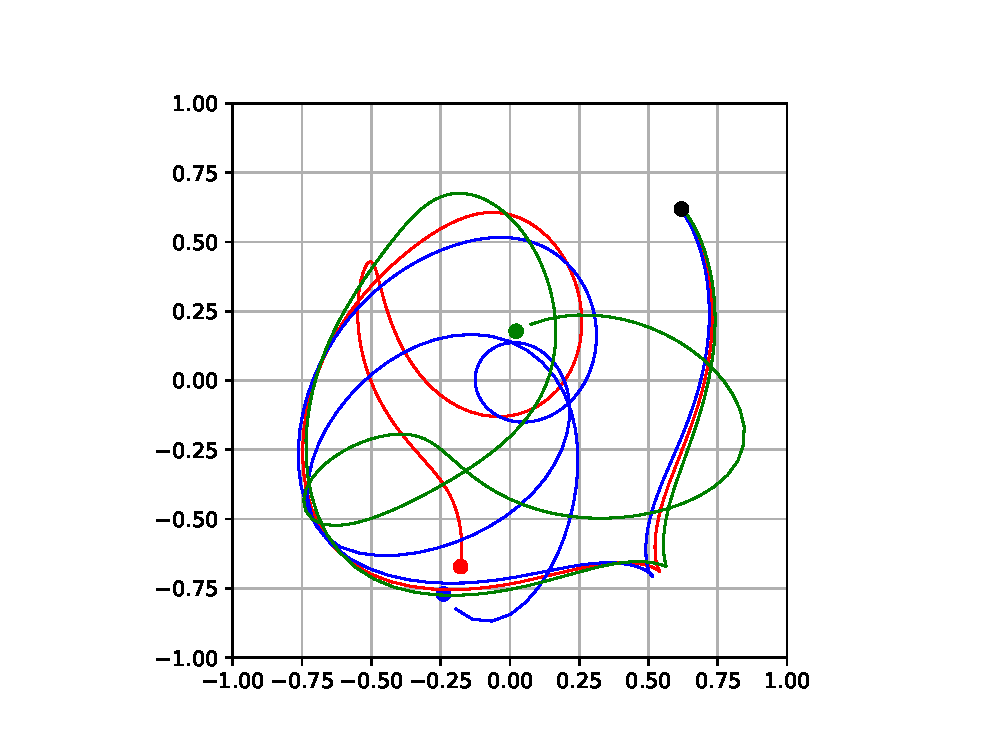
\includegraphics[scale=0.8]{_dp_sdic.eps}
    \captionof{figure}{Three double pendulum heads with equal angular velocity and initial angles differing by 0,025 radians}\label{fig:dp_sdic}
  \end{figure}

\end{Example}


The second part in Devaney's definition of chaos concerns topological transitivity.

\begin{Definition}
  [\bf {Topologically Transitive}]\label{Dfn_TopolTrans}\rm
	A dynamical system $F: U \to U$ is topologically transitive if for any pair of nonempty open sets $E_1$ and $E_2$ there exists a $n\in\mathbb{N}$ such that $T^n(E_1) \cap E_2 \not= \emptyset$. 
\end{Definition}

Topologically transitivity implies that the iterates of an open set of initial conditions gets mixed up with other open sets. On a compact metric space, it can be shown that topological transitivity also implies the existence of a point whose forward iterates are dense \cite{de2013elements}; or in other words, the orbit going through this point will be dense in the compact metric space. 
In fact, it is topologically more likely that the choice of an arbitrary point will be one  whose iterates are almost dense. 

\begin{Definition}
  [\bf {Meager Set}]\label{Dfn_Meager Set}\rm
A subset of a topological space $U$ is said to be a meager set if it can be written as a countable union of sets of with empty interior. The complement of the a meager set is set to be a residual set.
\end{Definition}

To be more precise (see \cite{de2013elements}), for a discrete-time dynamical system on a compact space, the set of points with dense iterates are residual, and they are typical or likely to be observed in practice. In this thesis, we assume that when data is observed from a topologically transitive system, we assume that the data arises from a dense orbit. 


We may now define the notion of Chaos as formulated by Devaney\cite{devaney2018introduction}.
\begin{Definition}
  [\bf {Devaney's Chaos}]\label{Dfn_ChaosDec}\rm
	A dynamical system $T: U \to U$ is said to exhibit chaos in the sense of Devaney if it satisfies the three properties:
	\vspace{-5mm}
  \begin{enumerate}
		\item $T$ has SDIC.
		\item $T$ is topologically transitive.
		\item The set of periodic points of $T$ are dense in $U$. 
	\end{enumerate}
\end{Definition}




\begin{Example} 
  The standard tent map $Tu=1-|2u-1|$ defined on $[0,1]$ is a well-known example of a dynamical system satisfying these three properties. 

  We now reason as to why this is true. The graph of the map $T$ is piecewise linear with two straight lines, one connecting the points $(0,0)$ and $(\frac{1}{2},1)$ and the other connecting $(\frac{1}{2},1)$ with $(1,0)$. They form a so-called tent with base centered at $u=1/2$. The graph of the map $T^2$ comprises two symmetric tents with their base centered at $1/4$ and $3/4$. See Figure \ref{fig:T2tentmap}

  \begin{figure}[ht]
    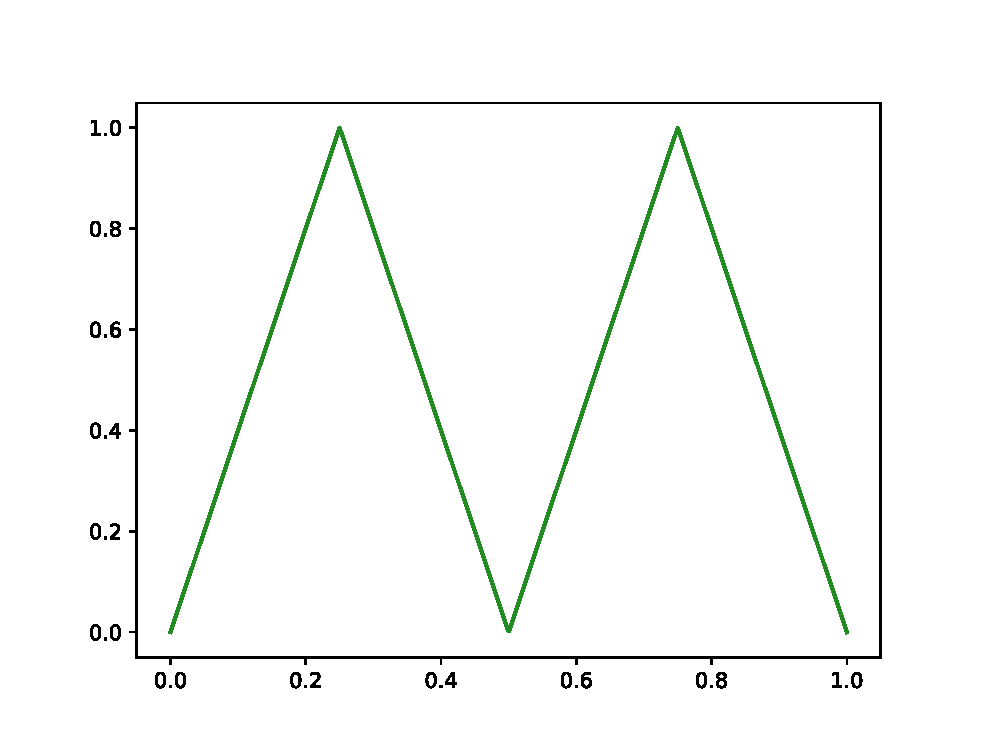
\includegraphics[scale=0.6]{_tentmap_2.eps}
        \centering
        \captionof{figure}{Graph of the $T^2$ map with bases at $x=0$, $x=\frac{1}{2}$ and $x=1$ respectively.}\label{fig:T2tentmap}
  \end{figure}
  
  In general, the graph of  $T^k$ contains $2^{k-1}$ tents.
  Given any point $u$ and an open neighborhood $W \subset[0,1]$ of $u$, we can find $k\in\mathbb{Z}$ large enough so that $T^k(W) = [0,1]$ because we can accommodate a tent whose base is contained in $W$.
  This implies the existence of two points $w_1$ and $w_2$ in $W$ so that $d(T^kw_1,T^kw_2)= 1$, and by the triangle inequality  at least one of the inequalities $d(T^ku,T^kw_1)> \delta$ or $d(T^ku,T^kw_2)> \delta$ hold when $\delta\in (0,\frac{1}{2})$.  So $T$ has sensitive dependence on initial conditions.
  
  Next, let $W_1$ and $W_2$ be two nonempty open sets. Given any open set $W_1$, we can find a $k\in\mathbb{N}$ large enough so that $T^k(W_1) = [0,1]$ because we can accommodate a tent with base contained in $W$. So $T^k(W_1) \cap W_2 \not=\emptyset$, and thus $T$ has topological transitivity.
  
  Finally, for every open interval $(a,b)$, the graph of $T^k$ intersects the graph of the identity map on $[0,1]$. This follows from the fact established above that there exists a $k\in\mathbb{N}$ such that $T^k(a,b) = [0,1]$.If the intersection point has coordinates of the form $(p,p)$, the point $p$ is then a fixed point of $T^k$ and therefore also a periodic point of $T$. Since we have found a periodic point in the interval $W$,  the set of periodic points are dense in $T$.
  This follows because any fixed point of $T^k$ is also a periodic point, and we have found this in an arbitrary interval.


\end{Example}




\section{Conjugacy}

We now turn our attention to the subject of conjugacy that describes when two dynamical systems are equivalent dynamically. 

To show topological similarity or sameness between two metric or topological spaces, one needs to establish a homeomorphism between the two spaces. 
However, in the study of dynamical systems defined on two spaces, establishing a homeomorphism does not indicate that the systems are dynamically related in any way.  For instance, the maps $Tu=u^2$ and $Tu=1-|2u-1|$ defined on $[0,1]$ have totally different behaviour. 
To find systems that are dynamically similar, one rather needs to establish a kind of dynamical equivalence which we illustrate in a simple commutativity diagram below.

% Giving errors
\begin{equation}  \label{eqn_conjugacy}
%    \[ 
    \psset{arrows=->, arrowinset=0.25, linewidth=0.6pt, nodesep=3pt, labelsep=2pt, rowsep=0.7cm, colsep = 1.1cm, shortput =tablr}
 \everypsbox{\scriptstyle}
 \begin{psmatrix}
U & U\\%
V & V.
 %%%
%  \ncline{1,1}{1,2}^{T} 
%  \ncline{1,1}{2,1} <{\phi}
%   \ncline{2,1}{2,2}^{S}
%  \ncline{1,2}{2,2} > {\phi}
 \end{psmatrix}
% \]
\end{equation} 

%Composite functions
To understand the diagram we note that if we travel ``right and then down," the diagram instructs us to use $T$ (top arrow right) first, followed by $\phi$. (right arrow downwards). Consequently the pathway amounts to finding $\phi(T(u))$. If we proceed "down and then right", the diagram instructs us to apply $\phi$ (left arrow downwards) first, and then apply $S$ (bottom arrow right). This then amounts to finding  $S(\phi(u))$. When the relationships in this diagram hold, we say $\phi(T(u))= S(\phi(u))$, and we formally denote it as $\phi \circ T=S\circ \phi$.

\begin{Definition}\rm  
[\bf {Conjugacy \& Semi-Conjugacy}]\label{Dfn_Conjugate}\rm
   Consider the dynamical systems $T:U\to{U}$, $S:V\to{V}$ and suppose the relationship $\phi \circ T=S\circ \phi$ holds. If $\phi:U\to{V}$ is a homeomorphism, then $S$ is said to be conjugate to $T$ and $\phi$ is called a conjugacy. If we relax the criterion on $\phi$ and merely require $\phi$ to be continuous and surjective where $\phi:U\to{V}$, then $\phi$ is a semi-conjugacy between $T$ and $S$ where T has domain $U$ and S has domain $V$; S is said to be semi-conjugate to T. 
\end{Definition} 

\ednote{M: Saying $\phi$ is then a semi-conjugacy between $T$ and $S$ could be ambiguous as it does not specify which system is on the top in the commutativity. So please edit accordingly. B: Does defining explicitly the domain and codomain of $\phi$ make it clear enough? }
When $S$ is conjugate to $T$, the dynamics of the two systems are in some way ''dynamically equivalent''. Specifically, they are in one-to-one correspondence with one another. However when $S$ is semi-conjugate to $T$ with $\phi:U\to{V}$ a many-to-one mapping, the dynamics on $V$ provide merely a coarse-grained description of the dynamics on $U$ \cite{de2013elements}. When $S$ is semi-conjugate to $T$, it is also common to call $S$ a \emph{factor of $T$}, or conversely that $T$ is an \emph{extension of $S$}. In essence, an extension (e.g., \cite{de2013elements}) is a larger system capturing all of the important dynamics of its factor.

It is a very hard or nearly an impossible task to establish the existence of a conjugacy or a semi-conjugacy $\phi$ between two systems \cite{devaney2018introduction}. However, one can verify that a function $\phi$ satisfies the commutativity diagram \ref{eqn_conjugacy}.  

\begin{Example}\rm
  For example $\phi(x)=\sin\big(\frac{\pi}{2}x\big)^2$ is a conjugacy between two systems $Tu=1-|2u-1|$ and $Sv=4v(1-v)$  defined on $U=[0,1]$.  

  Indeed, $\phi:[0,1]\to[0,1]$ is a homeomorphism and by employing simple trigonometric identities, it is easily proved that $\phi$ satisfies~\ref{eqn_conjugacy}
  \[
    \begin{aligned}[t]
      (\phi\circ{T})u 
                &=\sin^{2}\Big(\frac{\pi}{2} - \frac{\pi}{2}|2u-1|\Big) = \sin^{2}(\pi{u})=\Big(2\sin(\frac{\pi}{2})\cos(\frac{\pi}{2})\Big)^{2}=4\sin^{2}(\frac{\pi}{2}u)\Big(1-\sin^{2}\frac{\pi}{2}u\Big) \\
                                    &=({S}\circ\phi)u.
    \end{aligned}
\]
And it follows that $\phi$ is a conjugacy between the two systems.
\end{Example}


In establishing that two systems are conjugate (semi-conjugate) to one another, we have also shown that one may choose to work with one system as opposed to the second and still be guaranteed to obtain information on the latter. This is especially useful while forecasting the future evolution of dynamical systems. 


\chapter{The Learning Problem}\label{ch3}

In this chapter we acquaint ourselves with the question of forecasting dynamical systems with unknown underlying structures, state and discuss the shortcomings of the Takens delay embedding theorem and discuss various issues faced while forecasting. 

Consider a relatively simple learning problem: 
Given the sequence $(u_0, u_1, \ldots, u_m)$ for $m\in\mathbb{Z}$, a finite segment of an orbit of the map $T$ where $T$ is defined by the update equation $u_{n+1} = Tu_n$, forecast the values $u_{m+1}, u_{m+1}$ where the map $T$ is unknown, given that $u_m$. 

A practical example of this would be the subsequent scenario: given the time-sequential coordinates of an object moving in space, predict the future positions of that object. However we are very rarely, if at all, presented with a problem where the entire state information is available to us in the form $u_n$ at some time-step $n\in\mathbb{N}$. Consider then a more involved learning problem:

Suppose we only have the observations $\theta(u_0), \theta(u_1), \ldots, \theta(u_m)$ of the true system states $u$ in an unknown dynamical system $(U,T)$ and we wish to predict the values $\theta(u_{m+1}), \theta(u_{m+2})$ and so forth.

First we establish the method of Takens delay embedding. 
In this method, one considers a discrete-time dynamical system defined on a 'nice' space (a smooth manifold)\ednote{Should this manifold be further explained?} that can be obtained as time-$K$ map of a continuous time-dynamical system, concepts which will be formalised below.
We make observations from such a system, i.e., we observe the evolution of $\theta(w_0)$ (where $w_0$ represents the initial state) i.e., we observe  a finite set of values of $u_n :=  \theta(w_n) = \theta(Tw_{n-1})$. The sequence $\{u_n\}$ represents a scalar time-series and intuitively $\theta$ may be thought to represent a probe inserted into a larger system which is itself only measuring/extracting a small part of the greater system state at time $t=n$. 
Consider for example a thermometer erected to measure the ambient temperature in a local village. This measurement function, the thermometer, is capturing only a single aspect, the temperature, of a much grander dynamical system entailing the present weather of the surrounding area. Even more than that though- it is measuring a miniscule part of the global weather system. 


%Given the sequence $\{u_1, u_2, \ldots, u_n}$, we define the variable \newline $y_n:=[\theta_n, \theta_{n-\tau}, \ldots, \theta_{n-(2d-2)\tau}, \theta_{n-(2d-1)\tau}]^{T}\in\mathbb{R}_{d}\times{1}$ where $\tau$ represents the lag and $d$ the dimension of the attractor. (We shall return to these terms shortly and their discussion may be put on hold for the time being).

However, the true state $u$ of a system is seldom, if ever, fully known. In almost all cases we can at most insert probes into a system to obtain partial information by means of the measurements taken. Moreover, the process of taking a measurement itself introduces 2 additional aspects which complicate the problem: \ednote{M: Maybe replace difficulty by saying that we need to consider two aspects. B: Perhaps this edit makes more sense?}
\vspace{-8mm}
\begin{enumerate}[noitemsep, label=\roman*.]
  \item A series of measurements over a specific time-interval is inherently a discretisation procedure of the underlying continuous-time dynamical system. (Hence why we restricted our attention to discrete-time systems in the preceding section)
  \item A probe will never be fully accurate, and so the act of measurement introduces a certain measure of numerical noise/inaccuracy.
\end{enumerate}



From here we construct a multidimensional observable using the method of stacking previous observations, i.e., we create delay-coordinate map defined by
$\Phi_{k,\theta}(w) := (\theta(T^{-k}w)\ldots,\theta(T^{-1}w),\theta(w))$.  
The concept of an observable is understood in the sense of an observable as originally introduced by \cite{takens1981detecting, genericObservableAeyels} to refer to a probe or measurement function inserted into the system. 
The essence of Takens' theorem relates to the fact that when $k$ is sufficiently large, we can define a dynamical system on the space $\mathbb{R}^{k+1}$ whose states are $\Phi_{k,\theta}(w)$, $\Phi_{k,\theta}(Tw)$, $\Phi_{k,\theta}(T^2w)$, etc. and this dynamical system is topologically conjugate to the unknown underlying system $(W,T)$. We recall the Takens delay embedding theorem next.


%We may then ask ourselves the question: Is it in any way possible to retain information about the system state $x(t)$ in this temporal data-series $\theta(x(t))$? The answer is easily yes if T is known. However, neither this, nor even the exact function $\theta$ is available. 

\section{Takens Embedding Theorem}\label{sect_Takens}

We define first the concepts of homeomorphism and embedding:
\begin{Definition}\rm
  [\bf {Homeomorphism}]\label{Dfn_homeo}\rm
  A homeomorphism is a function $f:Z\rightarrow Y$ between two topological spaces $Z$ and $Y$ that is continuous, bijective and has a continuous inverse. 
\end{Definition}

\begin{Definition}
  [\bf {Embedding}]\label{Dfn_embed}\rm
  Consider a homeomorphism $f:Z\rightarrow Y$ for $Y\subset X$. $Z$ is said to be embedded in $X$ by $f$.
\end{Definition}

Takens Theorem states a result establishing a relationship between the observed and underlying dynamical systems by showing that the concatenation of a sufficiently large number of previous observations into a vector will, under certain conditions, generate a map between the vectors from the respective systems.  We formulate the theorem from \cite{takens1981detecting}.  

\begin{Theorem} 
	[\bf Takens Embedding Theorem (adopted from \cite{takens1981detecting}] \label{Thm_Takens}
         Let $W$ be a compact manifold of dimension $m$, and $d\ge m$ so that $2d$ is an integer. It is a 
            generic property for the pair $(T, \theta)$,  where $T:W \to W$ is
            a smooth diffeomorphism, and $\theta:W \to \mathbb{R}$ a smooth function, the map $\Phi_{2d,\theta}:W \to \mathbb{R}^{2d+1}$ defined on $W$ by 
            $\Phi_{2d,\theta}(w) := (\theta(T^{-2d}w)\ldots,\theta(T^{-1}w),\theta(w))$
            is a diffeomorphic embedding; by `smooth' we mean at least $C^2$. Consequently, there exists a map $F_\theta: \Phi_{2d,\theta}(W) \to \Phi_{2d,\theta}(W)$ defined by $$F_\theta: (\theta(T^{-2d}w),\ldots,\theta(T^{-1}w),\theta(w)) \mapsto 
            (\theta(T^{-2d+1}w),\ldots,\theta(w),\theta(Tw))$$
           so that $(W,T)$ is topologically conjugate to 
            $(\Phi_{2d,\theta}(W), F_\theta)$.    
\end{Theorem} 

By generic we mean a residual set on a certain topology on appropriate spaces of functions (that we do not describe here) \textbf{(Cite)}. 
By $C^2$, we make reference to a twice-differentiable function  with a continuous second derivative. In our scenario (and this remains important throughout) the input space $U$ is considered the attractor.~\label{attractor_U}

Below we reproduce Figure 1 from \cite{Supp}.

%Some explanation is beneficial. Takens establishes a delay-coordinate map $\Ftheta$ defined in \ref{eqn_takens} for $T$ the flow (\ref{defn_flow}) defined by the update equation  $Tu_n=u_{n+1}$ and $theta$ our measurement function. When confining a dynamical system to the manifold U (in which the underlying system is contained), Takens showed that if certain smoothness conditions are satisfied on $T$ and $\theta$, then the delay-coordinate map $\Ftheta$ embeds $U$ in the reconstruction space $R^{2d+1}$ \textbf{we haven't used the term reconstruction space yet, so this is falling out of the blue}, for almost every choice of measurement function $\theta$, the observable. By almost every choice here, we mean that we exclude some observations which do not give any information. To see a more precise discussion, see \textbf{xxx} for we do not concern ourselves with a further elaboration on this report.

%Alternatively we may also make the statement: Takens' Embedding Theorem guarantees that almost all dynamical systems can be reconstructed from just one noiseless observation sequence \textbf{this isn't obvious from the theorem's formulation, is it?} i.e. for a great number of possible observation functions $\theta$, $\Ftheta$ preserves the topology of U. \textbf{'preserving the topology' is not something we've touched on before. Perhaps I should add to previous discussion so logic flows seamlessly here}.

\begin{figure}[ht]
  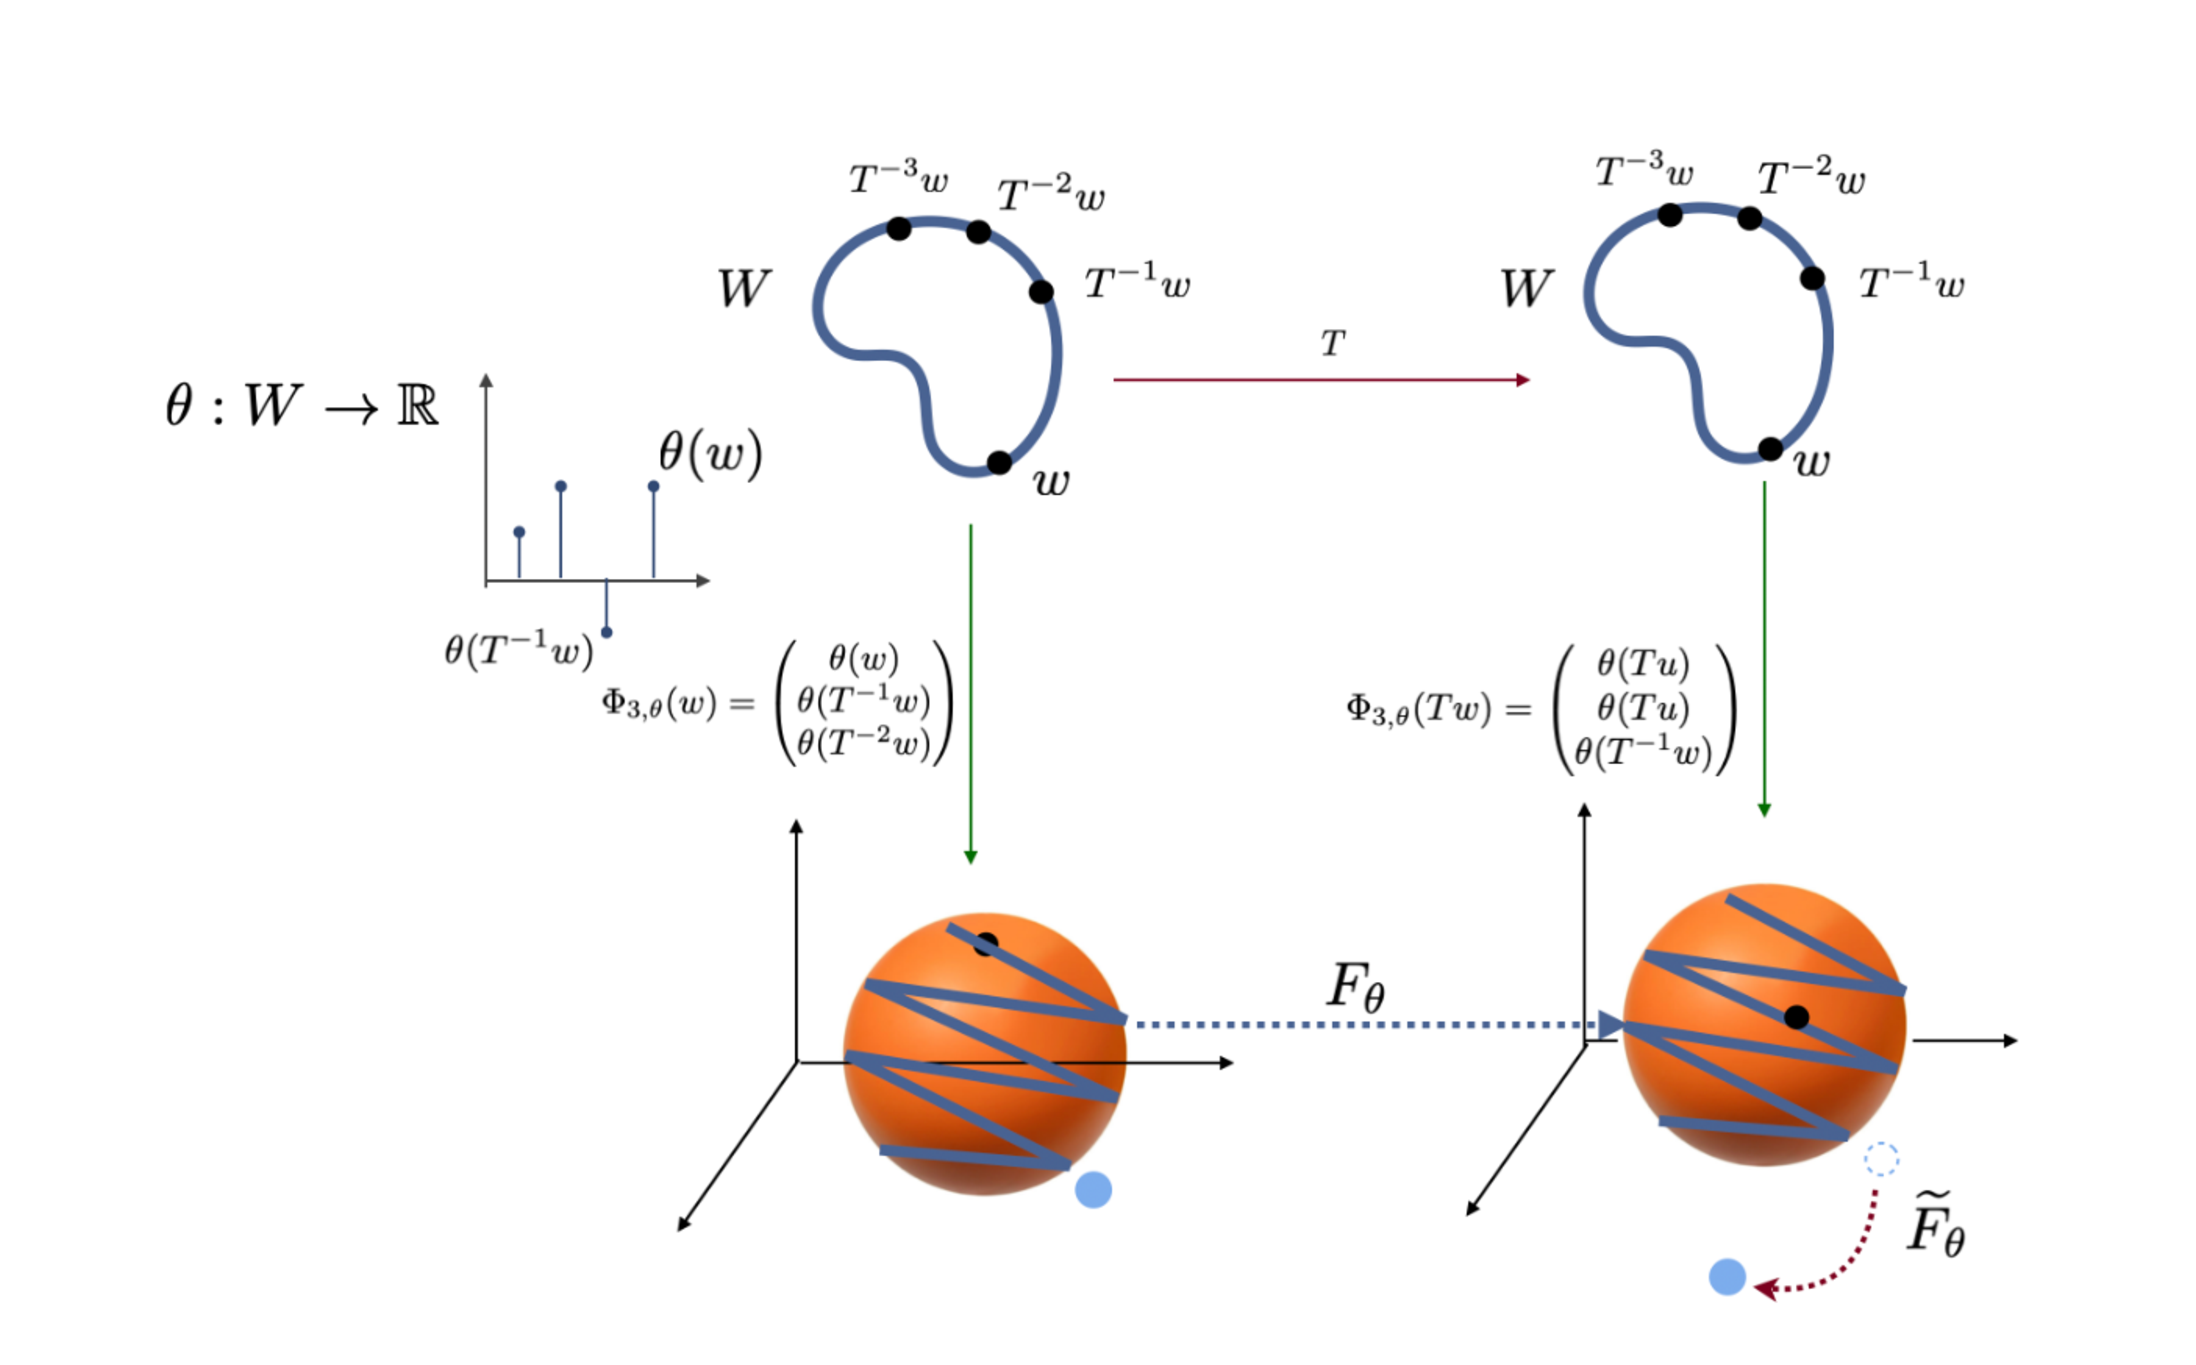
\includegraphics[scale=0.25]{_takensmap.eps}
  \centering
  \captionof{figure}{Schematic of Takens Embedding Theorem's usage and impact of iterates slipping from the attractor when the approximation $\tilde{F}_\theta$ of $F_\theta$ is learnt.}
  \label{fig:takensmap}
\end{figure}

If we can learn the map $F_\theta$, from sufficient number of data points of $\{\phi_{2d,\theta}(w_n)\}$, then we also know how to forecast how $\theta(w_n)$. 


%Once again we pause and consider the graph to consolidate our understanding of the conjugacy (\textbf{are we being too simplistic?}). If we are in state $u$ and then evolve towards state $Tu$ before embedding into $\mathbb{R}^{2m-1}$, then this is equivalent to first embedding into $\mathbb{R}^{2m-1}$ and then evolving through the map $\Ftheta$, i.e. $\Phi_{2d,\theta}\circ{F}_{\theta} = T\circ\Phi_{2d,\theta}$. The map $F_theta$ is a homeomorphism as well. 

%Thus information about U can be retained in the time series' (or observation's) output. By preserving the topology on the manifold $U$ in the reconstruction space $X$ (\textbf{not discussed before}), we are also guaranteed the preservation of topological invariants of the manifold, of which dimensionality is one such invariant. (We note here that dimensionality will again be considered later in this project).

\section{Practical Limitations to Takens' Theorem}

It is a fact that Takens' Embedding Theorem is both a powerful result and that it provides compelling reason to believe that one could conceivably reconstruct accurately a system conjugate to the underlying system. Nonetheless, it does present some serious practical limitations:
\vspace{-5mm}
\begin{enumerate}
\item Even supposing that we could indeed find $F_\theta$ , our \emph{approximation} of  $F_\theta$ is a map from a larger set $\mathbb{R}^{2d+1}$ containing the embedded attractor. There are, however, no theoretical guarantees that $F_\theta$ will retain  $V=\Phi_{2d,\theta}(W)$  as an attractor although $W$ could itself be an attractor.
\item Takens theorem is stated only for noiseless observations. Due to noise $\epsilon_n$ the delay vector $\Phi_{2d,\theta}(w_n) + \epsilon_n$  may lie outside $V$.Furthermore, due to the chaotic nature of the underlying system (i.e. the fact that it has SIDC), the evolution of $\Phi_{2d,\theta}(w_n) + \epsilon_n$ under the map $F_\theta$ could move out of $V$ completely. This problem can be overcome  by using a driven dynamical system with some properties, and we discuss this in Chapter\ref{ch3}. 
\end{enumerate}

The Takens embedding theorem does not guarantee global dissipativity.
\ednote{B:Links with~\ref{subs_LearnGamma} in discussion of dissipativity of $\Gamma$.  Sir, I'm not sure how to write this here - I think it a beneficial point to make so as to set the stage for the later discussion in ~\ref{subs_LearnGamma}, but I am unsure there as well.}


\ednote{Include note on learning failure because of sensitivity as in graph commented out?}
% \begin{figure}[ht]
%   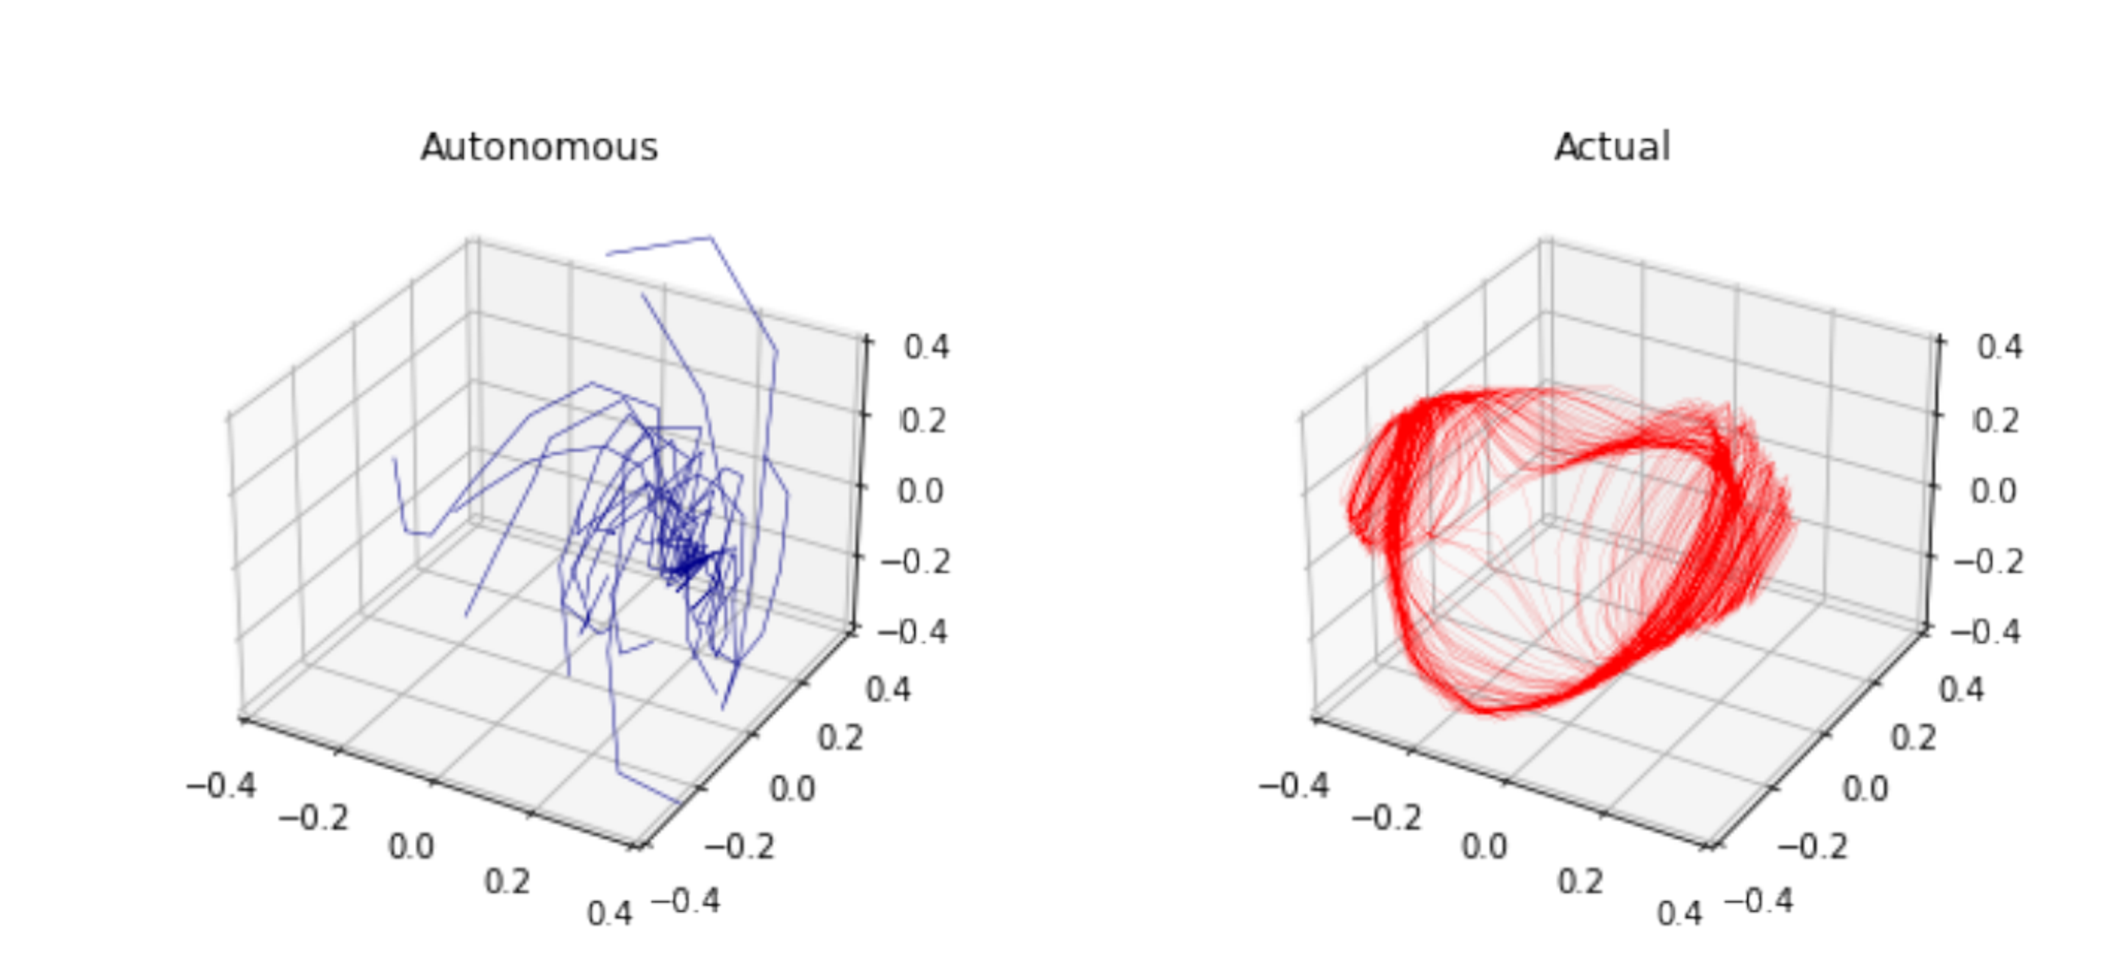
\includegraphics[scale=0.3]{_learningfailure.eps}
%   \centering
%   \caption{Illustration of a system having failed to learn the map}
%   \label{fig:supp_learning_failure}
% \end{figure}

Though not a uniquely related to the Takens embedding theorem, we do opt to make mention of this requirement for our work. 
The methods described here are applicable for data originating from a surjective map. 
This follows from the fact that when $T$ maps the space $U$ into a proper subset $B$ of $U$, we me conclude that $T$ is not surjective as there exists some point in $U-A$ which does not have a preimage.
An example of this would be the case when a system displays energy-loss. Consider, for instance, consider the oscillations dying down for a damped pendulum. (A more in-depth account will be given in \ref{ch5})

This requirement is not overly restrictive, as a great number of chaotic systems do have a surjective map. (Cite) \ednote{B: I remember you saying this in one of our sessions, but don't have a source for it.}


\chapter{Driven Dynamical Systems to Forecast Problems}\label{ch4}

In this chapter, we discuss results pertaining to the mapping of temporal data obtained from a discrete-dynamical system onto a different space through the notion of a driven dynamical system. 
We also consider the conditions a driven system should possess to avoid adding distortion to its state-space representation. We then describe the \emph{single-delay dynamics} (SDD) of the system and and finally recall conditions on the driven system so that the SDD are conjugate (or at least semi-conjugate) to the underlying system. 
The SDD can then be used to forecast and reconstruct the underlying system. 

\section{Nonautonomous and Driven Dynamical Systems}

\begin{Definition}
  [\bf Nonautonomous Dynamical System (adopted from~\cite{Manju_ESP})]\label{Dfn_NDS}\rm
  A nonautonomous dynamical system (NDS) on a space $X$ is simply a dynamical system comprising a family of maps $\{g_n\}_{n \in \mathbb{Z}}$ where $g_n(\ldotp):=g(u_n,\ldotp):X\to{X}$ is continuous. Each $g_n$ arises as a consequence of an input $u_n$ from the input space $U$, a topological space. 
\end{Definition}

We immediately recall the figure first defined in \eqref{eqn_conjugacy}  and remind ourselves of our ultimate goal to learn a system that is conjugate to an underlying or unknown dynamical system $(U,T)$ by making use of the measurements obtained from  the unknown system.

%#####################################
\begin{center}
\psset{arrows=->, arrowinset=0.25, linewidth=0.6pt, nodesep=3pt, labelsep=2pt, rowsep=0.7cm, colsep = 1.1cm, shortput =tablr}
\everypsbox{\scriptstyle}
\begin{psmatrix}
U & U\\%
V & V.
%%%
%  \ncline{1,1}{1,2}^{T} 
%  \ncline{1,1}{2,1} <{\phi}
%   \ncline{2,1}{2,2}^{S}
%  \ncline{1,2}{2,2} > {\phi}
\end{psmatrix}
%#####################################
\end{center}

To find a function $\phi$, the need now arises to consider a so-called driven dynamical system, one that can generate a  nonautonomous dynamical system, where two spaces are considered: input is taken from an input space $U$ and the state of a space $X$ is updated. (Previously, only the state was considered.)
We do this to mimic the true conditions. By accounting for an extrogenous input sequence in $U$ which can also influence the  system-state at a specific time-step, it produces more general models than an autonomous system.

\begin{Definition}
  [\bf Driven, Compactly Driven Dynamical System] \label{Dfn_DDS} \rm
A driven dynamical system comprises two topological metric spaces $U$, $X$ and a continuous function  $g:U\times{X}\to{X}$ where $g(u_n, x_n)=x_{n+1}$.
If the input space $U$ is compact, we refer to the system as compactly driven. 
\end{Definition}

The dynamics on X are generated by the update equation $x_{n+1}=g(u_n, x_n)$ where $n\in\mathbb{Z}$, input $u_n$ from $U$ and state $x_n$ belonging to $X$, where $X$ is compact.
Abbreviated, we shall refer only to the \emph{driven system $g$}, with all other entities being understood implicitly.

Notably, a nonautonomous dynamical system may be generated from $U$; any input $\overline{u}$, a bi-infinite sequence from $U$, gives rise to the sequence of self-maps $\{g(u_n, \cdot)\}_{n\in\mathbb{Z}}$ contained in $X$.
Physically, one may think of this bi-infinite sequence as referring to a system that has been running for a long period at the time of the first measurement taken from the system (alternatively, the first time a probe is inserted into the system to take an observation)

\begin{Definition}
  [\bf Entire Solution] \label{Dfn_Soln} \rm
  A sequence $\{x_n\}_{n\in\mathbb{Z}}\subset X$ is called an entire solution (or simply a solution) of the driven system  $g$ with input $\overline{u}$ when it satisfies 
  \[g(u_{n-1}, x_{n-1})=x_n\] for all $n\in\mathbb{Z}$
\end{Definition}

It is important to emphasise that a sequence $\{x_n\}$ satisfying the update equation above can only be a solution if $x_n\in{U}$ holds for all $n\in\mathbb{Z}$ and just for $n>0$. Consider the example below.

\begin{Example} \rm \label{ex_halfux}
  The only solution  $\{x_n\}_{n\in\mathbb{Z}}$ to the driven system  $g(u,x)=\frac{ux}{2}$, where $X=[0,1]$, $U=[0,1]$,  is the zero solution $x_n\equiv0$.
  To see this, consider any $x_n=a\in[0,1]$ where $a\neq{0}$.  Let $\overline{u}\in{U}$ be an non-zero constant sequence , say $u_n=0.5$. 
  The driven system may be rewritten as $x_{n-1}=\frac{2x_n}{u_{n-1}}=4x_n$ and the  iterates of $x_n$ in backward time will increase by a factor of 4 at each timestep. 
  Thus for some $m\leq{n}$,  $1<x_m$ i.e. $x_m\notin{X}$. So ${\{x_n\}}_{n\in\mathbb{Z}}$ is not a solution and it follows that the only possible solution is the zero solution.
\end{Example}


A system may also have multiple solutions as is evidenced in the example below.

\begin{Example}\label{Ex_exp} \rm 
  Consider the driven system $g(u,x)=x^2$ for $X=[0,1]$, $U=\mathbb{R}$. The system has an uncountable number of solutions, as there exists a solution for every $x\in{X}$ which also passes through the point $x$ and $lim_{n\to\infty}x_n=0$, $lim_{n\to{-}\infty}x_n=1$.  
 The proof is deferred to immediately after the next paragraph (see~\ref{rem_proofEx}).
\end{Example}

As the solutions to a driven system are often considered to be an important entity \cite{M: edited the sentence here}, we next identify a subspace $X_U$ of $X$ that contains all possible solutions. To realize such a subspace of a driven system $g$, the concept of a reachable set is defined.

\begin{Definition}
  [\bf Reachable Set]\label{Dfn_ReachableSet}\rm
The reachable set of a driven system $g$ is exactly the union of all the elements of all the (entire) solutions, i.e., 
\[X_U :=\Big \{x \in X:  x = x_k \mbox{ where  $\{x_n\}$  is a solution for some  $\bar{u}$} \Big \}.\]
The set of all reachable states at a specific time $n$ for input $\overline{u}$ is denoted by $X_n(\overline{u})$
\end{Definition}

The reachable set itself can defined independently from the fact that $g$ does or does not have the USP. We note that $x\in{X_n(\overline{u})}$ if and only $g$ has a solution $\{x_k\}$ for $x_n=x$ and input $\overline{u}$. \textbf{(Cite)}.
The set $X_n(\overline{u})$ is exactly the set of all points $x$ that have some entire solution $\Psi$ passes through it at time $n$. \ednote{B: Changed sentence for better readability - still understandable?} 

We can give an alternate formulation of the set $X_n(\overline{u})$:
suppose, for some fixed input 
$\overline{u}$, we define $g_i = g(u_i,\cdot)$ for all $i\in \mathbb{Z}$, then the set of states
\begin{equation} \label{eqn_association}
X_{n,i}(\overline{u}) := g_{n-1} \circ \cdots g_{i+1} \circ g_i(X).
\end{equation}

As the image of a finite composition of continuous maps, the set $X_{n,i}(\overline{u})$ is compact whenever $X$ is compact and is also nonempty.
Further, $X_{n,i}(\overline{u}) \supset X_{n,i-1}(\overline{u})$. Hence $\bigcap_{i<n}
X_{n,i}(\overline{u})$ is a nested intersection of closed nonempty subsets, and
whenever $X$ is compact, the intersection is nonempty.  \ednote{B: Should I cite here?}

\begin{Definition}
  [\bf Topological Contraction]\label{Dfn_TopContr}\rm
  We say $g$ is a topological contraction if $\bigcap_{i<n}X_{n,i}(\overline{u})$ is a singleton subset of $X$ for each $\overline{u}$. 
\end{Definition}

It turns out that $\bigcap_{i<n}X_{n,i}(\overline{u})$ is identically equal to $X_n(\overline{u})$ that we had defined earlier \textbf{(Cite.)}. This will lead to a result (for. e.g., \cite{manjunath2013echo}) that  \textit{$g$ being a topological contraction is equivalent to the existence of a exactly one entire solution.}

\begin{Remark}
  [\bf Proof of Example~\ref{Ex_exp}] \label{rem_proofEx} \rm
  For the driven system,  
  $g(u,x)=x^2$ the evolution does not depend on the input at all. Hence $g(u,x)$ can be written as a single map $f(x)=x^2$ which is a homeomorphism on $[0,1]$. A left-infinite orbit is defined and it converges to $1$ while the right-infinite orbit converges to $0$. Or in other words the iterates of $f^{-1}$ converges to $1$ while the iterates of $f$ converge to $0$ 
\end{Remark}

Thus far it has been demonstrated that a system may have one or more solutions; one may ask if a driven system always has a solution and, if so, whether it satisfies certain properties such as uniqueness. 
Should the driven system be compact, existence follows immediately.

\begin{Theorem}\label{Thm_CompactExistence}
 Let $g$ be a driven system.  If $X$ is compact, then for each input $\overline{u}$, there exists at least one solution to the driven system $g(\ldotp, x)$
\end{Theorem}
\begin{proof}
  May be found in \cite{kloeden2011nonautonomous, manjunath2014dynamics, manjunath2013echo}
\end{proof}

% One may easily construct many systems with trivial solution-sets, such as $g(u,x)=x$ which has only the constant solution $x$ and so for $U=[-1,1]$, the system would have no solution if $|x|>1$. To refine the scenario, we consider only systems with unique solutions. 

\section{Unique Solution Property}

\begin{Definition}
  [\bf Unique Solution Property] \label{Dfn_usp}\rm
  A driven system $g$ is said to have the Unique Solution Property (USP) if for each input $\overline{u}$ there exists exactly one solution. 
  Alternatively we may formulate the USP as follows: $g$ has the Unique Solution Property if there exists a well-defined map $\Psi:{U}\to{X}$, with $\Psi({\overline{u}})$ denoting the unique solution.
\end{Definition}

One of the first result obtained after defining the USP is the fact that every solution will attract different initial conditions towards the component parts of the solution. %, i.e. that the solution $\Psi$ is a non-autonomous uniform attractor. \ednote{Define Uniform Attractor before stating theorem or else omit the statement.} 
If $g$ has the USP, then any solution to $g$ is also a uniform attractor in nonautonomous dynamical systems literature \cite{Manju_Nonlinearity}. The discussion on nonautonomous attractors is beyond the scope of this project and we refer the reader to \cite{Manju_ESP, esann2012ids} for further reading. 

% Paraphrased. 
%Additionally, $g$ having the USP is in our context also equivalent to $g$ being a topological contraction \cite{manjunath2021universal}, or alternatively also that $g$ exhibits the Echo State Property (ESP). 

\ednote{RC introduced a bit abruptly} Reservoir Computing(RC) refers to a machine learning approach in which input is mapped onto a different, but higher dimensional, space through a system called the reservoir after which a readout measuring the reservoir state is trained.
In the majority of Reservoir Computing(RC) literature \textbf{(Cite)}, a notion of forgetting the states of the reservoir asymptotically is often used.  
Concepts like the echo state property(ESP) and  fading memory \cite{boyd1985fading} are two of these.  
If $g$ possesses the ESP (equivalent in our context to the USP \textbf{(Cite)}), we are guaranteed that the whole of an input's left-infinite history will exactly determine the current system state; i.e. there is only ever the possibility of a single reachable state at a given instance of time \cite{jaeger2001echo,Manju_2020}.
% \cite{Manju_ESP}.
Beyond forgetting the past states, the ESP is also often discussed in terms of a stability property that plays a key role in the robustness of recurrent neural networks(RNN).
The concept, termed input-related stability~\cite{manjunath2020stability}, refers the phenomenon of nearby inputs creating responses (solutions) close to one another.

\section{Establishing Conjugacies}

Having already defined the reachable set $X_U$ as the collection of all elements of all entire solutions, we pause briefly in order to fix additional notation.
Defining $\cev{u}^{n}:=(\ldots,u_{n-2} ,u_{n-1})$ as the left-infinite subsequence of an input up until time $n$, $\overleftarrow{U}$ is then the notation for all these left-infinite sequences in $U$. 
Moreover, $\cev{u}^{n}v:=(\ldots,u_{n-2} ,u_{n-1}, v)$ will symbolise the input up to time $n$ with $v \in U$ being the specific input value at time $n$. 
The introduction of a new input at time $n$ can be described by the mapping $\sigma_v:   \cev{u}^{n} \mapsto \cev{u}^{n}v$. 
The right-shift map, $r\overleftarrow{U}\to\overleftarrow{U}$, of an input sequence is defined $r: (\cdots, u_{-2},u_{-1}) \mapsto(\cdots, u_{-3},u_{-2})$

The goal now assumes the form of the question on our ability to establish a semi-conjugacy as presented below for the driven system $g$. 

\begin{equation}  \label{Scomm_h}
  %    \[ 
      \psset{arrows=->, arrowinset=0.25, linewidth=0.6pt, nodesep=3pt, labelsep=2pt, rowsep=0.7cm, colsep = 1.1cm, shortput =tablr}
   \everypsbox{\scriptstyle}
   \begin{psmatrix}
   \overleftarrow{U} & \overleftarrow{U}\\%
   X_U & X_U.
   %%%
  %  \ncline{1,1}{1,2}^{\sigma_v} \ncline{1,1}{2,1} <{h}
  %  \ncline{1,2}{2,2} > {h}
  %  \ncline{2,1}{2,2}^{g(v,\cdot)}
   \end{psmatrix}
  % \]
  \end{equation} 	


We proceed to consider a specific subclass of conjugacies.

  \begin{Definition}
    [\bf Universal Semi-Conjugacy]\label{Def_UnivSemiConj} \rm
    Given a driven system $g$, we  call a continuous and surjective map $h : \overleftarrow{U} \to X_U$ a universal semi-conjugacy if  diagram \ref{Scomm_h} commutes for all $v \in U$.
  \end{Definition}

  If the universal semi-conjugacy $h$ exists (i.e. the diagram in \ref{Scomm_h} commutes) then the solution $\Psi(\bar{u})$ will intuitively have no more ``complexity' than the input $\bar{u}$.

But does such a function $h$ for the above driven system $g$ above exist? Whenever $g$ has the USP and $\Psi(u)=\{x_n\}_{n\in\mathbb{Z}}$ it follows that $h$, defined by  $h(\cev{u}_n):=g(u_n,x_{n-1})=x_n$, will satisfy the semi-conjugacy in the graph above \ref{Scomm_h}.
Regrettably, such a continuous mapping $h$ is not guaranteed to exist \cite{M: Have edited here} when $g$ does not have the USP \cite[Lemma 5]{Manju_Nonlinearity}.
Note that even when $h$ does exist, we are not guaranteed its injectivity. Considering again example \ref{ex_halfux}, we see that even if $h$ were to exist, it could not be injective as $X_U=\{0\}$.

Re-sketching the commutativity diagram \ref{Scomm_h} above by replacing $X_U$ by its left-infinite sequence space $\overleftarrow{X}_U$, we obtain the diagram below. In this case, the function $H:\overleftarrow{U}\to\overleftarrow{X}_U$, a map that is both continuous and surjective, is called a \emph{causal mapping} that is defined next. 

\begin{Definition}
  [\bf Causal Mapping]\label{Def_CausMap}
  A continuous, surjective map $H:\overleftarrow{U}\to\overleftarrow{X}_U$ such that \[H\circ\tilde{g}_v=\sigma\circ{H}\] holds for all $v \in U$ where $\tilde{g}_v$ maps $(\ldots, u_{-2}, u_{-1})$ to $(\ldots, u_{-2}, u_{-1}, g(v, u_{-1}))$ is called a causal mapping.
\end{Definition}

\begin{equation} \label{SCausal_H}
    %    \[ 
        \psset{arrows=->, arrowinset=0.25, linewidth=0.6pt, nodesep=3pt, labelsep=2pt, rowsep=0.7cm, colsep = 1.1cm, shortput =tablr}
     \everypsbox{\scriptstyle}
     \begin{psmatrix}
     \overleftarrow{U} & \overleftarrow{U}\\%
     \overleftarrow{X}_U & \overleftarrow{X}_U.
     %%%
    %  \ncline{1,1}{1,2}^{\sigma_v} \ncline{1,1}{2,1} <{h}
    %  \ncline{1,2}{2,2} > {h}
    %  \ncline{2,1}{2,2}^{\tilde{g}_v}
     \end{psmatrix}
    % \]
  \end{equation} 	

 \begin{Theorem}
  For a compactly driven system, a causal mapping $H$ exists if and only if $g$ has the USP. 
\end{Theorem}
\begin{proof}
  See~\cite[Th.3]{manjunath2013echo}.
\end{proof}

The driven system $g$ can induce an embedding of $\overleftarrow{U}$ in $\overleftarrow{X}$ as follows: 
If the causal mapping $H:\overleftarrow{U}{\to}{\overleftarrow{X}_U}$ is injective (in addition to being surjective), it becomes the embedding of $\overleftarrow{U}$ in $\overleftarrow{X}$ induced by the driven system $g$. 
The continuity of $H^{-1}$ follows from the fact that $H$ is itself a continuous and surjective mapping of a compact space $\overleftarrow{U}$ in a Hausdorff space.
and we refer to the map $H$ as a \emph{causal embedding}.

When $g$ has the USP, the diagram below (adopted from~\cite{Manju_Nonlinearity}) illustrates the operation of the mappings $h$ and $H$. The mapping $h:\overleftarrow{U}\to{X_U}$ is also considered an observable as mentioned in the introduction of Chapter \ref{ch3}).  

\begin{figure}[ht]
  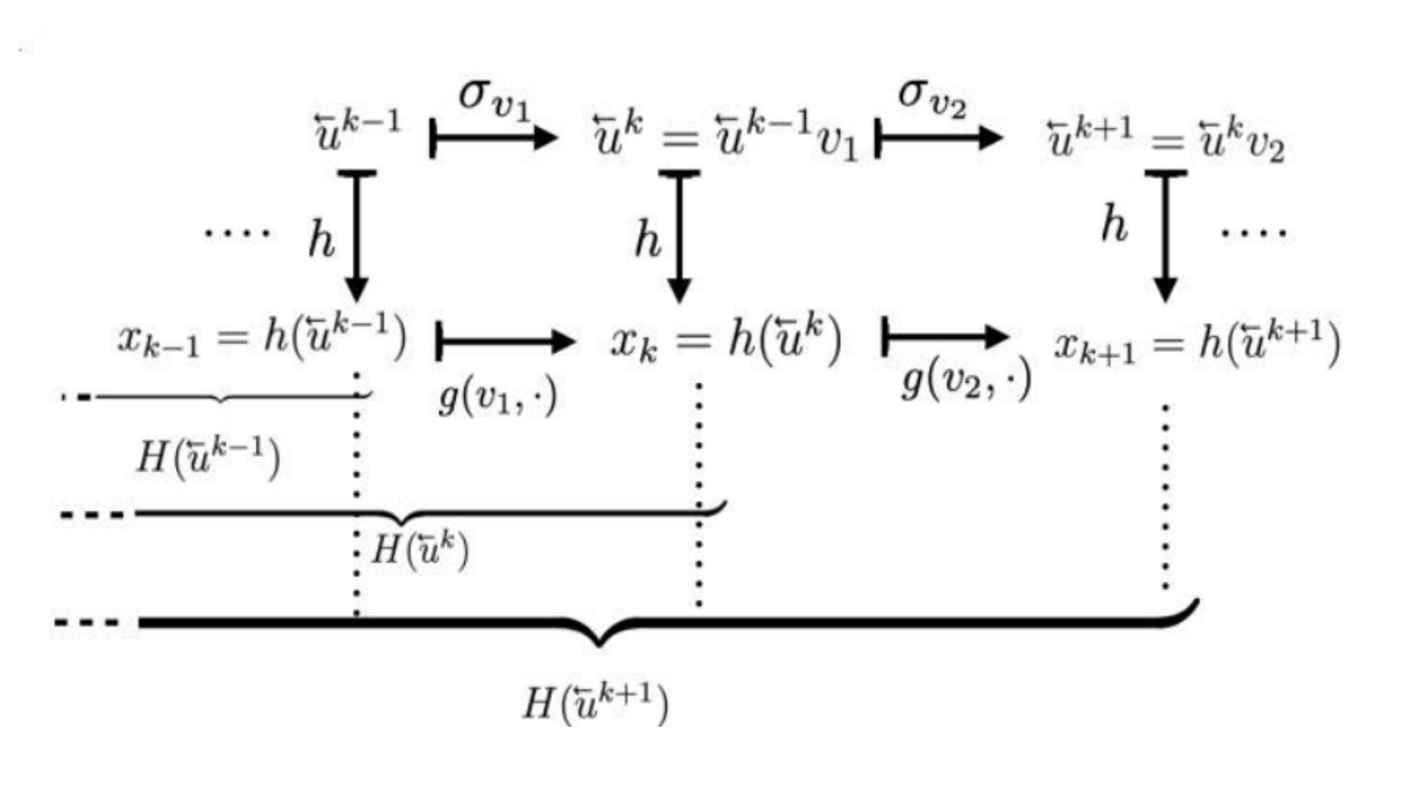
\includegraphics[scale=0.4]{_actionofh_H.eps}
  \centering
  \captionof{figure}{Ladder-like behaviour of $h$ and $H$ to illustrate the causal mapping. (Figure reproduced from~\cite{Manju_Nonlinearity}) }
  \label{fig:actionh_H}
\end{figure}

The function $H$ contains a countably infinite number of coordinate (or factor maps) since its codomain is $\overleftarrow{X}_U$.  
As it is not practically feasible to consider a left-infinite sequence in $X_U$ (in other words an element of  $\overleftarrow{X}_U$) for learning, we wish to restrict the inputs we consider to a subspace of $\overleftarrow{U}$. 
Particularly, we restrict our attention to the  so-called inverse-limit space of a dynamical system and hope to embed it within some finite product of $X$. 

%We wish to explore the possibility of establishing a conjugacy rather than a mere semi-conjugacy and therefore are interested in the restriction of inputs to the left-infinite orbits of a dynamical system.

The left-infinite orbit space is significant because a great amount of information about the original system can be gleaned from its topological structure~\cite{ingram2011inverse,Manju_IEEE}. 
The formal topological structure for the inverse-limit space of a chaotic dynamical system is complicated, and further discussion is relegated to~\cite{kennedy2008inverse_limit, ingram2011inverse}.
Broadly, we may conceive of the inverse-limit system of a dynamical system as a subspace of an infinite-dimensional space where each point in the inverse-limit space corresponds to a backward orbit of the map $T$. 
Following~\cite{manjunath2021universal, ingram2011inverse} we provide a definition:

\begin{Definition}
  [\bf Inverse-Limit Space, Inverse-Limit System]\label{Dfn_InverseL}\rm
 The subset $\widehat{U}_T\subset \overleftarrow{U}$ defined by \[\widehat{U}_T: = \{ (\ldots,u_{-2},u_{-1}): Tu_{i} = u_{i+1}\} \] is called the inverse-limit space of $(U,T)$.
 The self-map $\widehat{T}$  induced by $T$ on $\widehat{U}_T$  is defined by \[\widehat{T}: (\ldots,u_{-2},u_{-1}) \mapsto  (\ldots,u_{-2},u_{-1},T(u_{-1}))\] and the resulting dynamical system $(\widehat{U_T}, \widehat{T})$ is called the inverse-limit system of $(U,T)$.
\end{Definition}

The inverse-limit space is well-defined since $T : U \to{U}$ is surjective by assumption.We now get to the concept of embedding the inverse limit-space of the dynamical system in $X \times X$. 

\begin{Definition} \rm
	We say a driven system $g$ \emph{causally embeds} a dynamical system $(U,T)$ if it satisfies the two properties: (i) a universal semi-conjugacy exists and  (ii)  $H_2(\cev{u}) := (h(r\cev{u}),h(\cev{u}))$ embeds the inverse-limit space $\widehat{U}_T$ in $X \times X$. \end{Definition} 

It is imperative to take note of a subtlety here: we refer to the \emph{map} $H$ as a (causal) embedding, whereas the driven \emph{system} $g$ (causally) embeds another \emph{system} $(U,T)$.


\section{Choosing the driven system $g$}

So far it is not clear if the USP alone ensures the ability to causally embedding a dynamical system and we mention that a driving function $g$ cannot just be chosen in a frivolous manner. This could possibly complicate our work. \ednote{Dié lees vreemd}

%The driving function $g$ cannot be chosen in a frivolous manner as it could possibly complicate our work. Specifically, one must be careful to avoid a choice of $g$ which would  add complexity to the obtained solution.  

%When a causal embedding $H$ exists for the driven system $g$, one can map an arbitrary input ${u}$ onto the solution space $X$ without additional distortion or information-loss \textbf{(Cite.)}.


%When an embedding is established, the question of possible additional complexity in the solution is removed by guaranteeing that, since the systems are conjugate (semi-conjugate, \textbf{(refer)}), $g$ does not add any (some) complexity to the system.  

%To achieve a causal embedding embedding not just a causal mapping, it is undesirable to choose a function $g$ that quenches the temporal structure in $u$ by contracting to such a degree that the ability to recover information from the original system is lost completely.
In the above example(\ref{ex_halfux}), the input's temporal variation could not be related to the reachable set as $X_U$ only consisted of a single element; little, if not no, information is encoded.
To obtain a suitably complex function $g$, it is thus desired that the reachable set of a driven system  be large enough to relate to the input. 
This is true even for embedding  the inverse-limit space of a dynamical system. \textbf{(B: Expand or refer?)}


 To this end, we recall the notion of State-Input (SI) Invertibility.  

\begin{Definition}
  [\bf SI-Invertibility]\label{Dfn_SIinv}\rm
  A driven system $g$ is said to be SI-Invertible if $g(*,x): U \to X$ is invertible for all $x\in X$. Alternatively it may be said that if, given $x_n$ and $x_{n-1}$, $u_{n-1}$ can be uniquely determined from $x_n=g(u_n,x_{n-1})$, then $g$ is said to be SI-invertible.
\end{Definition}
 
SI-invertibility means that one's choice of $g$ will still ensure 'enough' information is retained without introducing unwanted complexity. 
'Enough' here refers to the fact that we may always recover the previous input value $u_n$ (if we know successive states $x_{n-1}, x_n$).

Subsequently we define the relation $Y_T$ induced by $(U,T)$ on $X_U\times{X_U}$ for a driven system $g$ possessing SI-invertibility.  
To describe the  SDD formally, we consider a dynamical system $T: U \to U$ and define a relation on the reachable set $X_U$, i.e. a subset on $X_U \times X_U$  defined by 
$$Y_T:=\{(x_{n-1},x_n): \{x_k\}_{k\in \mathbb{Z}} \mbox{ is a solution for some orbit of } T \mbox{ and } n \in \mathbb{Z}\}.$$ 

The following theorem establishes the existence of a well-defined map $G_T$ describing the SDD of the system above. 

\begin{Theorem}
If we let $G_T:Y_T\to{Y_T}$ be a map defined by the relation $(x_{n-1},x_n)\mapsto(x_n,x_{n-1})$, then $G_T$ is well-defined (and this results holds even in the absence of $g$ possessing over the USP)  
\end{Theorem}
\begin{proof}
  \textbf{See .....................}
\end{proof}



%'Without additional complexity' is guaranteed by the invertibility of the function $g$ that guarantees a one-to-one mapping between $u_n, x_{n-1}$ and $x_n$. In obtaining an SI-invertible function, therefore, we are guaranteed a system which will not lose so much information about its previous states in the forward-flow of time that one may not make any credible claims as to the original system's behaviour and properties. Simultaneously, it does guarantee us that the important information encoded in previous inputs is indeed preserved.

At this stage it is worth taking note of a specific driven system in the form of a discrete state-space model which has acquired some adherence in applications \cite{Manju_IEEE}- especially those pertaining to Echo State Networks and the ESP. The function 
\begin{equation}  \label{eqn_driving}
  g(u,x) = (1-a)x + a\overline{\tanh}(Au + \alpha Bx)
\end{equation} 
is SI-invertible and, if $\alpha B$ has a spectral norm $<1$, also possesses the USP \cite[Th.2]{manjunath2013echo }. 
It is easy to show that $g$ is SI-invertible by recovering $u_n$ in 
\begin{equation} \label{eqn_SI_RNN}
  u_{n-1} := A^{-1}\bigg(\overline{\tanh}^{^{-1}}\frac{1}{a}\Big(x_{n+1}-(1-a)x_n\Big) \bigg) - \alpha B x_n
  \end{equation}
  when $x_{n-1}$ and $x_n$ are known.


This specific driving function $g$ is used in our implementation and is discussed more completely in chapter~\ref{ch5}

Despite the ease that with which one manipulates a left-infinite history in the realm of theory, it is impossible to obtain or use such a sequence in any real-life application.  
Fortunately, one does not need the entire left-infinite history of an input in practice thanks to the Uniform Attraction Property(UAP). 
We use an alternate version of the definition of UAP -- since the notion of nonautonomous attractors in this thesis would take some time to establish and detracts from the principal thrust of this project, we refer to \cite{Manju_Nonlinearity}. 


\begin{Definition}
  [\bf Uniform Attraction Property]\label{Dfn_UAP}\rm
  A driven system $g$ has the uniform attraction property (UAP) if we initialize the driven system
with an arbitrary initial value $y_m \in X$, and the sequence $y_{m+1}, y_{m+2}, y_{m+3},...$ satisfying $y_{k+1}= g(u_k,y_k)$ for $k \geq m$ then approximates an actual solution $\{x_n\}$ uniformly in the sense that given $\epsilon>0$ (independent of $y_m$) there is an integer $n$ so that $d(x_{n+i}, y_{n+i})<\epsilon$ for all $i\ge 0$, where $\{x_m\}$ is a solution.
\end{Definition}

The UAP guarantees that all trajectories will converge to the same trajectory as time moves forward. An illustration of this is shown in Fig.~\ref{fig:memloss_conttime} where the trajectory in red locks on to the supposed actual solution when the system has the USP.

\begin{figure}[ht]
  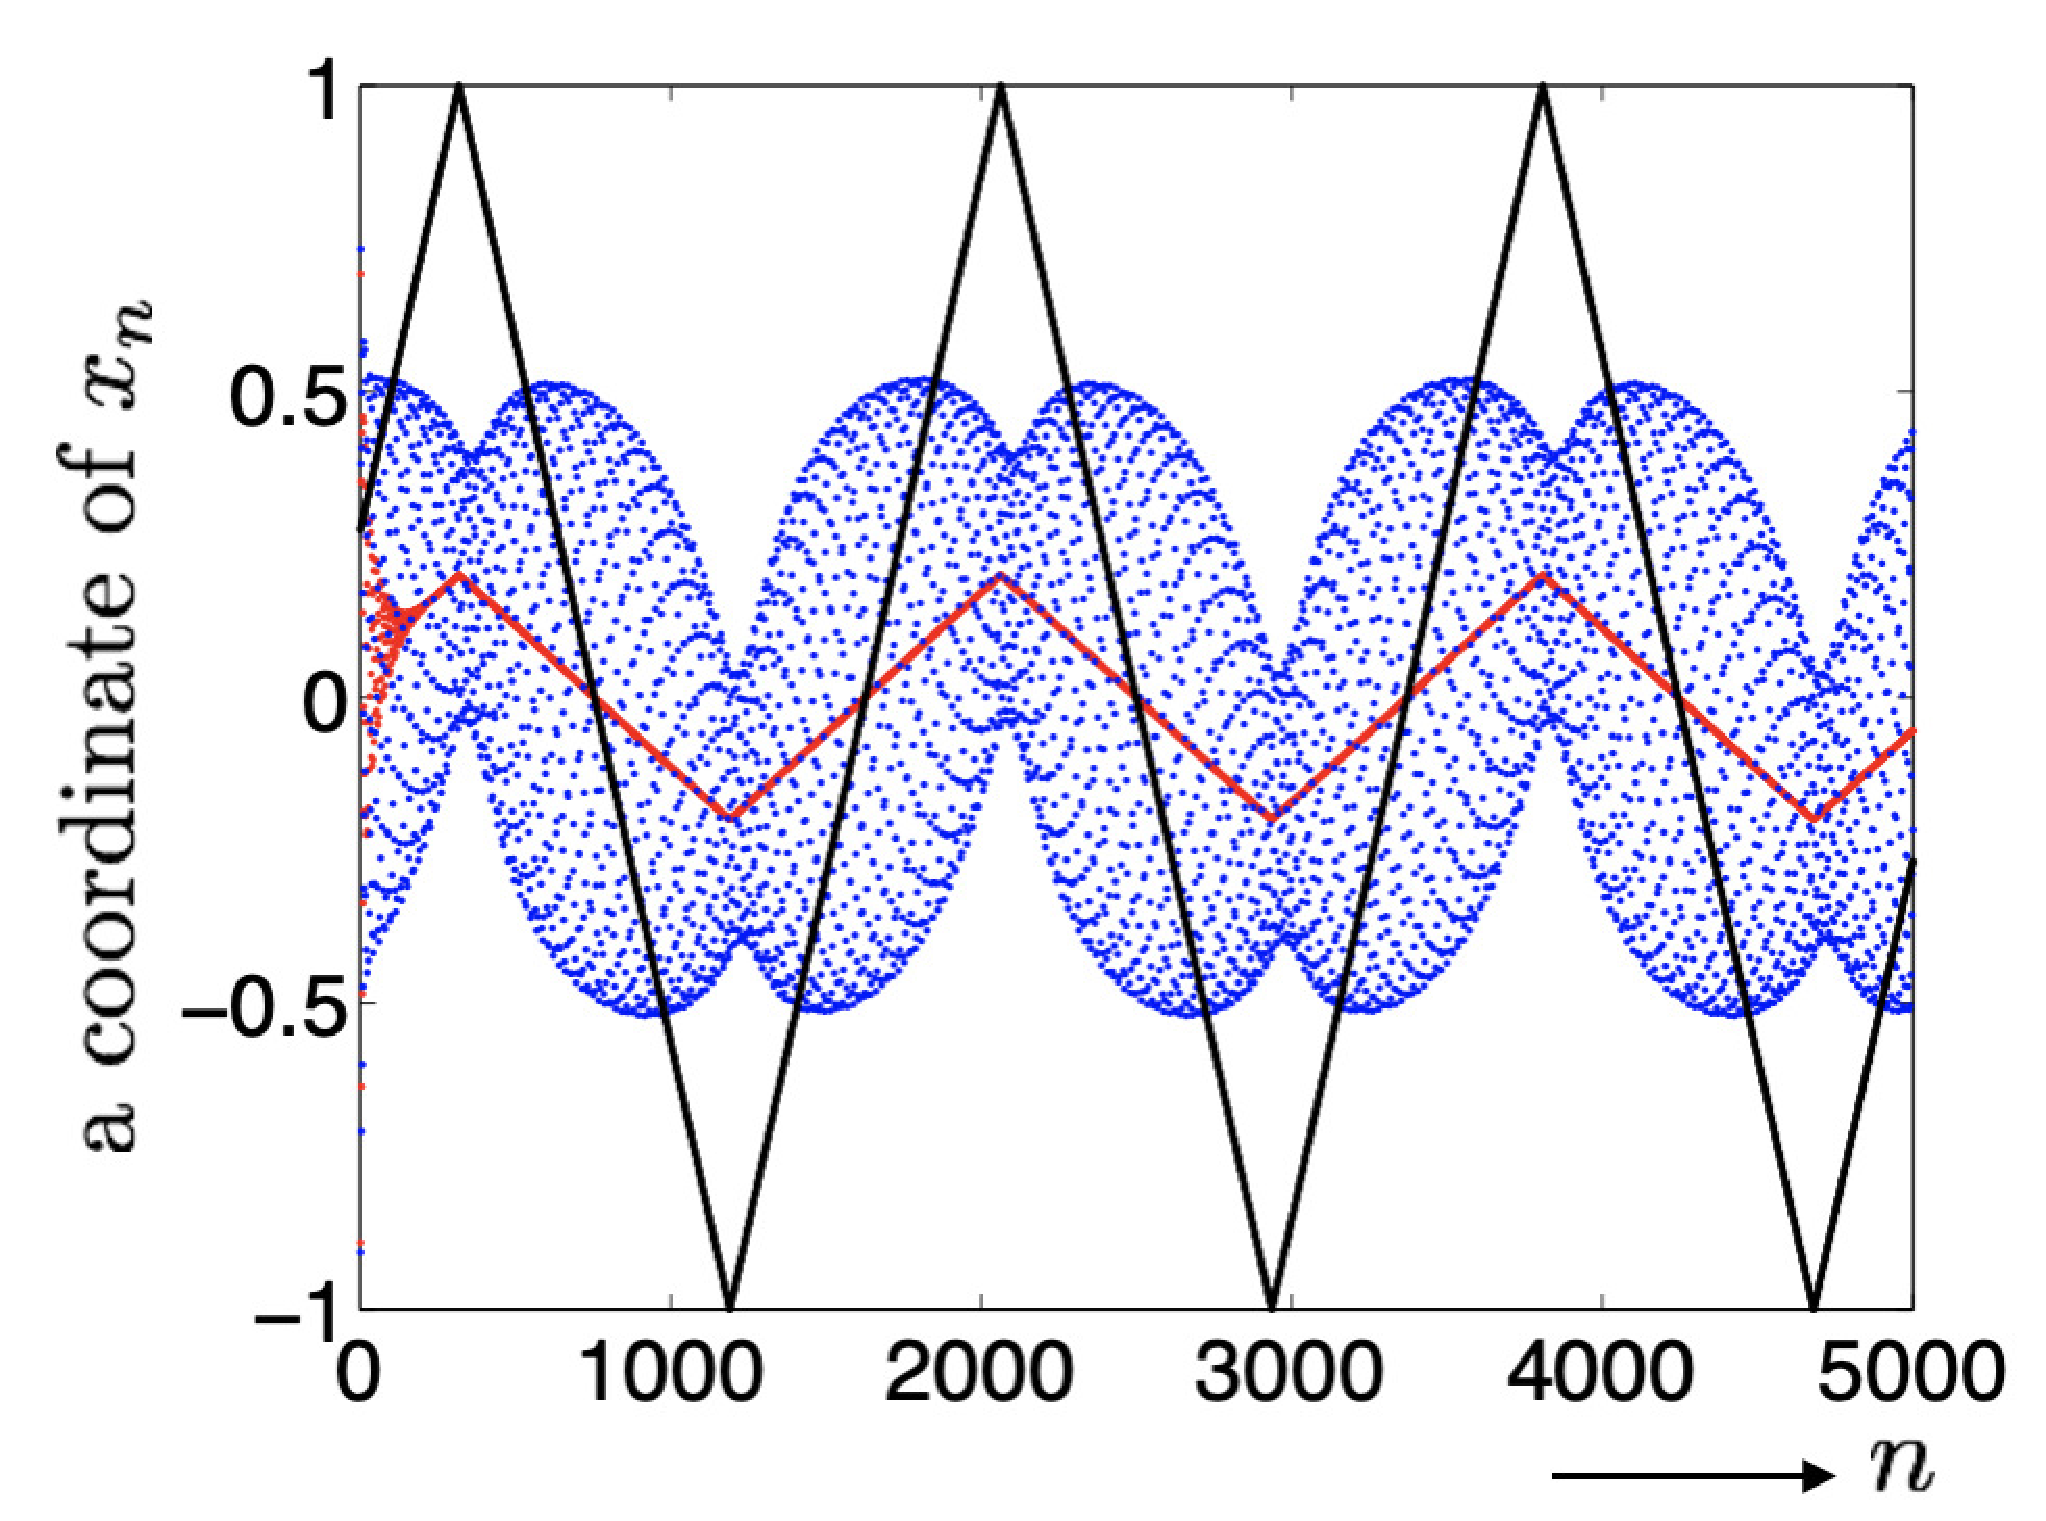
\includegraphics[scale=0.35]{_Nonlinearity_Fig_response.eps}
  \centering
\captionof{figure}{A coordinate of a simulated solution $(x_0,x_1,\ldots,x_{5000})$ of a RNN  plotted in red (with parameter $\alpha=0.99$ (where $g$ has the USP) and blue ($a=1$ and $\alpha=1.05$ where $g$ does not have the USP) while the matrices $A$ and $B$ are randomly generated, and $B$ has unit spectral radius. Reproduced from \cite{Manju_Nonlinearity}.}
\label{fig:memloss_conttime} 
\end{figure} \ednote{This graph with the black line does not immediately make sense}

One may now appreciate an even more astounding result: $g$ having the USP is equivalent to the UAP as is proved in~\cite{Manju_Nonlinearity}.


%We restate the above theorem.

%\begin{Theorem}\label{thm_usp-contr-uap}  The following statements are equivalent:  \vspace{-8mm}  \begin{enumerate}[noitemsep, label=\roman*.]    \item $g$ has the USP.    \item $g$ is a topological contraction.    \item $g$ has the UAP.  \end{enumerate\end{Theorem}\begin{proof}  May be found in \cite[Th.1]{Manju_Nonlinearity}\end{proof}

% One need therefore not establish any additional results to ensure that the sequence uniformly approaches the unique solution $\Psi$. This vastly simplifies the effort necessary to set up a problem in order to guarantee that the underlying system will be accurately represented by the conjugate system.

%This also solves the problem of perturbation/noise introduced by the observable or measurement function. Recall from before that an observable is inherently a map that discretises the underlying continuous-time system. Moreover, measurement and device error introduce mistakes. Since we are working with a chaotic system displaying sensitive dependence on initial conditions, these small errors could potentially send the trajectory into a completely different attractor. 
%In the presence of the UAP, however, small measurement errors introduced into the system do not pose the same danger as before since the trajectories will eventually tend towards the actual solution.
% \ednote{(B: Is this Complete enough?)}
% \textbf{From the perspective of perturbation of an autonomous dynamical system, if the resulting nonautonomous system has the USP, then the temporal structure of noise relates to the dynamics on a nonautonomous uniform attractor through a topological semi-conjugacy or a conjugacy.}

\section{The next step in Dynamics}


% Recall that $g$ is only being given inputs from the orbits of $T$.  


%Incredibly, this permits one to initialise a driven system $g$ with an altogether arbitrary initial value $y_m\in{X}$ where $m\in\mathbb{Z}$ and the UAP then guarantees that the sequence $\{y_{m+1}, y_{m+2},\ldots\}$ which satisfies the relation $y_n=g(u_n, y_{n-1})$  for  $k\geq{m}$  will approach the elements $\{x_n\}$ of the actual solution. This vastly simplifies the effort necessary to set up a problem in order to guarantee that the underlying system will be accurately represented by the conjugate system.

We are interested in determining whether $\widehat{T}$ and $G_T$ are related. For this, we introduce  the function $H_2{\overline{}} := (h(r\overline{u}, h(\overline{u})))$ mapping the entirety of a left-infinite sequence to some element in $X\times{X}$. 
Indeed, it may be shown that $g$ having SI-invertibility and the USP immediately guarantees the existence of at least a semi-conjugacy between the systems $(Y_T, G_T)$ and $(\widehat{U}_T, \widehat{T})$.
This is formalised in the Causal Embedding Theorem, which we state next:

\begin{Theorem}
  [\bf Causal Embedding Theorem (adopted from \cite{Supp})]
  % {\bf (Causal Embedding Theorem.)}
 \label{Thm_CET}
	Let $g$ be a driven system with SI-invertibility and the USP. Let $h$ denote the universal semi-conjugacy and $H_2(\overleftarrow{u}) := (h(r\overleftarrow{u}),h(\overleftarrow{u}))$, where $r$ is the right-shift map. 
 Let $(\widehat{U}_T, \widehat{T})$  be the inverse-limit system of a dynamical system $(U,T)$. 
 Then the restriction of $H_2$ to $\widehat{U}_T$ is a topological semi-conjugacy between the inverse-limit system $(\widehat{U}_T, \widehat{T})$ 
and the induced dynamical system  $(Y_T,G_T)$, i.e., the following diagram commutes
\begin{equation} \label{comm_H_CET}
\psset{arrows=->, arrowinset=0.25, linewidth=0.6pt, nodesep=3pt, labelsep=2pt, rowsep=0.7cm, colsep = 1.1cm, shortput =tablr}
 \everypsbox{\scriptstyle}
 \begin{psmatrix}
 \widehat{U}_T & \widehat{U}_T\\%
 Y_T &  Y_T.
 %%%
%  \ncline{1,1}{1,2}^{\widehat{T}} \ncline{1,1}{2,1} <{H_2}
%  \ncline{1,2}{2,2} > {H_2}
%  \ncline{2,1}{2,2}^{G_T}
 \end{psmatrix}
 \end{equation}
or in other words, $(Y_T, G_T)$ is a factor of  $(\widehat{U}_T, \widehat{T})$. Further, if $T:U \to U$ is a homeomorphism, 
then $H_2$ embeds $\widehat{U}_T$ in $X_U \times X_U$, and hence $(Y_T, G_T)$ is conjugate to $(\widehat{U}_T, \widehat{T})$.
\end{Theorem}
\begin{proof}
  May be found as the proof of~\cite[Th.4]{Supp}
\end{proof}

Recall that $H_2$ maps an entire left-infinite solution sequence from $\Psi$ \ednote{Check}to an element in $X\times{X}$. 
\ednote{Rephrase}We are drawing nearer and nearer to our principal target and our results carry more and more weight. Since if learn $G_T$ we would have learnt $\widehat{T}$ and since $\widehat{T}$ is an extension of $T$, we would have learnt $T$ as well. 

\ednote{Why is theorem on inverse-limit system taken out?}
%\begin{Theorem} Graph \ref{Scomm_h} is exactly the inverse-limit system $(\hat{U}, \hat{T})$.    \end{Theorem}



%We now have the following (which may be compared with \ref{SCausal_H} above):

%\begin{equation} \label{fig:inverse_limsystem}
  %  \[       \psset{arrows=->, arrowinset=0.25, linewidth=0.6pt, nodesep=3pt, labelsep=2pt, rowsep=0.7cm, colsep = 1.1cm, shortput =tablr}      \everypsbox{\scriptstyle}
%      \begin{psmatrix}      \widehat{U}_T  && \widehat{U}_T \\     Y_T && Y_T \\
      %%%
     %  \ncline{1,1}{1,2}^{\widehat{T}} \ncline{1,1}{2,1} <{h}
     %  \ncline{1,2}{2,2} > {H_2}
     %  \ncline{2,1}{2,2}^{G_T}
%      \end{psmatrix}
    %  \]
%  \end{equation}
 

%\begin{Theorem}
 %   $(Y_T, G_T)$ is semi-conjugate to $(\widehat{U}, \widehat{T})$.
%\end{Theorem}
%\begin{proof}
%  See \cite[Th.3, Th.4]{manunath2021universal}
%\end{proof}


\section*{Summarising the discussing thus far:}

It is easy to lose the birds-eye view, so we take a moment to review our progress up until this point.

\vspace{-8mm}
\begin{enumerate}
\item We are interested in a some dynamical system $(U,T)$ with unknown dynamics.
\item To determine properties about this system $(U,T)$ and predict its future evolution, we determine the dynamics of the inverse-limit system $(\widehat{U}, \widehat{T})$.
% Given certain assumptions, we can guarantee that $(\widehat{U}, \widehat{T})$ is at least semi-conjugate to $(U,T)$.
\item If the driven system $g$ is SI-invertible (and $\{u_n\}\in{U}$  is an orbit of $T$), the map $G_T$ exists that describes the single delay dynamics. 
\item If, furthermore, $g$ has the USP, $(Y_T, G_T)$ is semi-conjugate to $(\widehat{U}, \widehat{T})$.
\item If we can assume that $T$ is a homeomorphism, $(Y_T, G_T)$ is topologically conjugate to $(\widehat{U}, \widehat{T})$, an extension space of $(U,T)$
\end{enumerate} 

One can therefore in practice learn the SDD of the driven system states via $G_T$ with enough data thanks to the USP/UAP. This enables us to do at least two things: 
\vspace{-8mm}
\begin{itemize}
\item Forecast  $x_{n+1},x_{n+2}, \ldots$ via iterates of $G_T$ (if $G_T$ can be learnt).
\item Forecast future values of $u_n$ since $x_n$ and $x_{n+1}$ determine $u_n$ since $g$ is SI-invertible. 
\end{itemize} 


Finally, we note that although $G_T$ exists with SI-invertibility, we need USP  otherwise the driven states has to be running for all time since the driven states would not have forgotten its past states. 

% Below is reproduced a pictorial representation of the relationship between different entities and properties. \textbf{(Cite SIG_25May)}
% Below is reproduced a pictorial representation of the relationship between the different entities and their properties.

\begin{figure}[ht]
  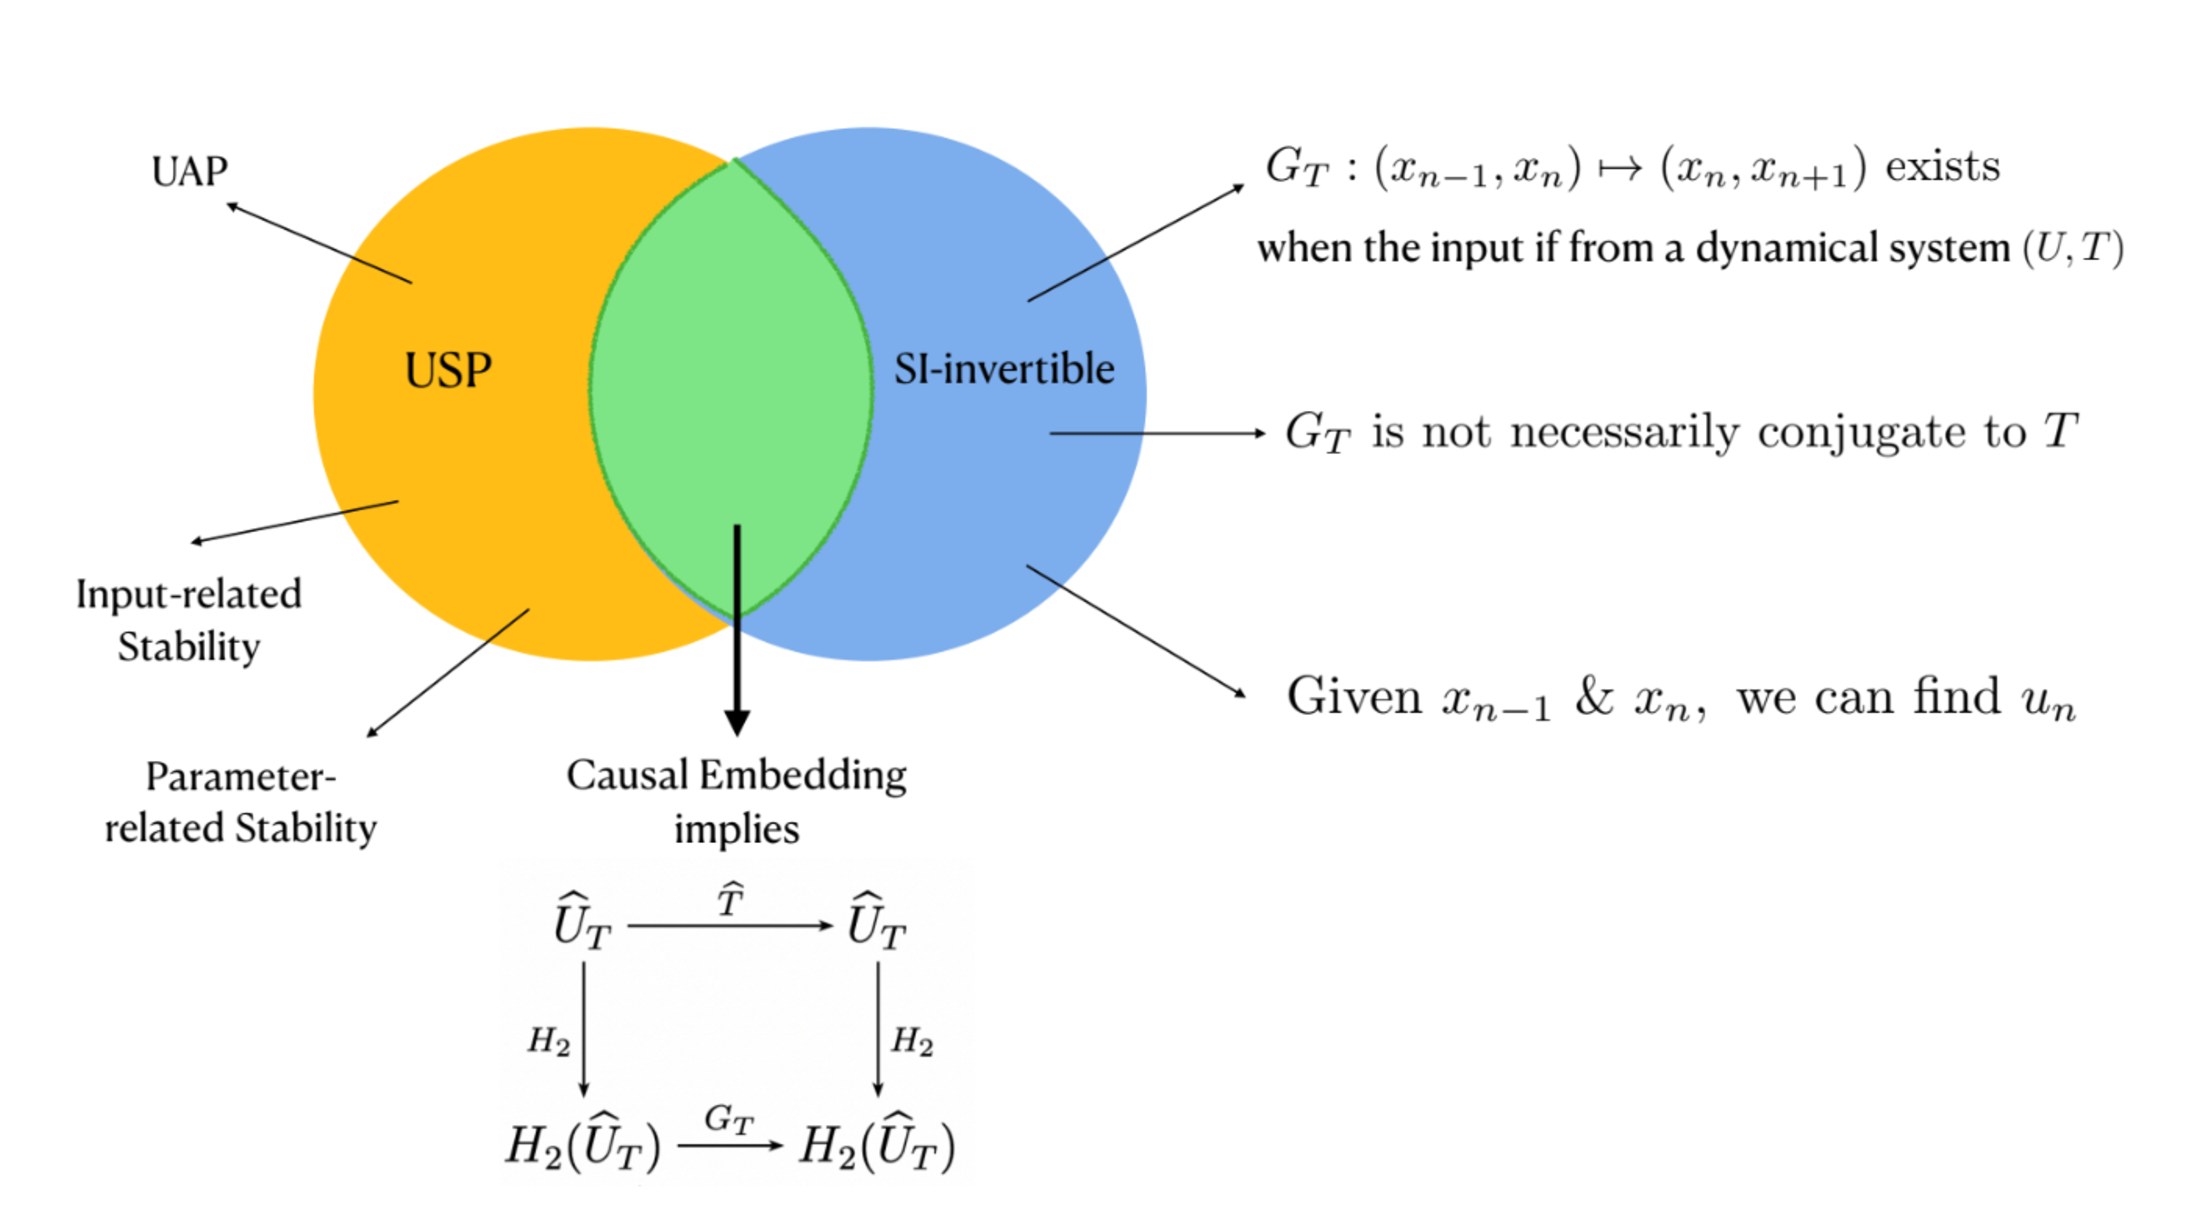
\includegraphics[scale=0.3]{_summarypictorial.eps}
  \centering
  \label{fig:fig_pictorialSummary}
\end{figure}
\ednote{M: Please put a caption on this figure and cite the figure in the main text}



\section{A discussion of $G_T$ }

In the above sections, we established the map $G_T$ describing the SDD of a driven system. By establishing the existence of this map, we’ve essentially embedded the attractor $U$ (recall from \ref{attractor_U}) into the higher dimensional space $X\times{X}$.
In layman’s terms, this ensures that there is more “dimensional room” for the underlying system’s underlying dynamics to “move”. Since the dynamics aren’t as “squashed”, we might therefore hope that the dynamics of $G_T$ are in some sense simpler than that of $T$. (Taken note of the fact that $G_T$ is a homeomorphism even when $T$ is just continuous)
 
In \cite{manjunath2021universal} it is illustrated in an empirical fashion in that the map $G_T$ describes dynamics which are less functionally complex than that of $T$ or of the map $\Phi_{2d,\theta}$. This is done by implementing a Recurrent Neural Network (RNN), which is discussed in~\ref{ch5}. \ednote{(B: Should I add in that we'll be using Pearson coefficient?)}
 
We opt to learn $G_T$ in an indirect manner by defining a new map $\Gamma:(x_{n-1},x_n)\mapsto{u_n}$. It will follow immediately from $G_T$’s existence that $\Gamma$ also exists. 

The reasons for taking this roundabout approach remain to be discussed in \ref{subs_LearnGamma}, but a pat answer may immediately be given: When $\Gamma$ has been learnt, the system can be driven autonomously and then $G_T$ is known anyway. We formalise this with a theorem.

\begin{Theorem}
  When $x_n$ and $x_{n-1}$ are successive points on a solution obtained for input-orbit of $T$ $\{u_n\}$, then the map $\Gamma: X\times{X}\to{U}$ defined by $(x_{n-1},x_n)\mapsto{u_n}$ exists whenever $G_T$ exists 
\end{Theorem}
\begin{proof}
  See \cite[Th. 3c]{manjunath2021universal}.
\end{proof}

Projection mappings $\pi_i$ are defined in the traditional meaning where a $k$-dimensional vector is projected to it's $i^{th}$ component such that $$\pi_i:(a_1,a_2, \ldotp, a_{k-1}, a_k)\to{a_i}$$

The graph in equation \ref{fig:comm_H_CET} is then extended as below:

\begin{equation}  \label{Scomm_imp}
  %    \[ 
      \psset{arrows=->, arrowinset=0.25, linewidth=0.6pt, nodesep=3pt, labelsep=2pt, rowsep=1.3cm, colsep = 1.1cm, shortput =tablr}
   \everypsbox{\scriptstyle}
   \begin{psmatrix}
   \widehat{U}_T & \widehat{U}_T\\%
   Y_T & Y_T\\
   & \textcolor{red}{U \times X}
   %%%
  %  \ncline{1,1}{1,2}^{\widehat{T}} \ncline{1,1}{2,1} <{H_2}
  %  \ncline{1,2}{2,2} > {H_2}
  %  \ncline{2,1}{2,2}^{G_T}
  %  \psset{linecolor=red}
  %  \textcolor{red}{\ncline{2,1}{3,2}<{(\Gamma,\pi_2)}}
  %  \ncline{3,2}{2,2}>{\textcolor{red}{(\pi_2,g)}}.
   \end{psmatrix}
  % \]
  \end{equation} 



The problem finally simplifies to the issue of learning the map $\Gamma$ and combining this with the projection mapping $\pi_2$ and the function $g$, which will be known. A final set of equations is obtained - equations that have been entirely constructed from data.
\begin{eqnarray}\label{eqns_from_data}
	u_{k+1} &=& \pi_1 \circ (\Gamma, \pi_2) \circ (\pi_2,g) (u_k,x_k) \label{Seqn_u}\\
	x_{k+1} &=& \pi_2 \circ (\Gamma, \pi_2) \circ (\pi_2,g) (u_k,x_k). \label{Seqn_x}
\end{eqnarray}



\section{Advantages of learning $\Gamma$} \label{subs_LearnGamma}

One may immediately ask why we opt to take such a roundabout route; why not just learn the map $G_T$ from the get-go? On the surface, this seems to be an arbitrary decision path with no real reasoning, so we take a pause again and discuss the motivation for learning Gamma.
There are a number of distinct advantages. 

In the first place, learning $\Gamma$ saves computational resources. This is due to the fact that the input $u_n$ lies in a lower-dimensional subspace in comparison to the high-dimensional space $X\times{X}$. 

%In practice, if the input is of a  lower dimension, one may easily embed it into the space $X\times{X}$ by padding the vector $u_n$ with zeroes.

Secondly, the function $\Gamma$ is known to be stable. Learning $\Gamma$ makes use of equations \ref{eqns_from_data} which in turn employs the driven system $g$ possessing the USP, and offers distinct advantages with regards to stability in the presence of perturbation. It is desirable that inputs that differ only slightly would have only ‘slight’ effects on the output of the system. Moreover, one would hope to prevent numerical errors originating from input and measurement noise (see~\cite[Th. 5]{manjunath2021universal}). 
As the data fed into the system is a function of both the input given and the parameters of the system itself (i.e. the value a, $\alpha$ in $\tanh$), we exploit both input-related and parameter-related stability. Both these notions are defined by way of the continuity of an encoding map of an input and design parameter respectively in \cite{manjunath2020stability}.\

Informally, we may consider input-related stability as concerned with the question of whether or not small variations in input would result in small responses.   
If two inputs $\bar{u}$ and $\bar{u}_{noisy}$ are close in the product topology, then their tails could differ greatly due to the metric that generates the product topology has insensitivity to the differences in sequence's tails.
 However if the system has the USP then the function $h$ is continuous and so $h(\bar{u}), h(\bar{u}_{noisy})$ remain close-by for small levels of noise maintaining a measure of robustness to input and measurement noise.\cite{manjunath2021universal}.
In a similar fashion, parameter-related stability is obtained thanks to a result \cite[Lemma 3.2]{manjunath2020stability} relating this form of stability with the ESP (which is here equivalent to the USP).


% Secondly,  due to $g$ possessing the USP, both input- and parameter-related stability~\cite{manjunath2020stability} is obtained, which in turn prevents numerical errors that caused by input and measurement noise (see~\cite[Th. 5]{manjunath2021universal}). 

\begin{figure}[ht]
  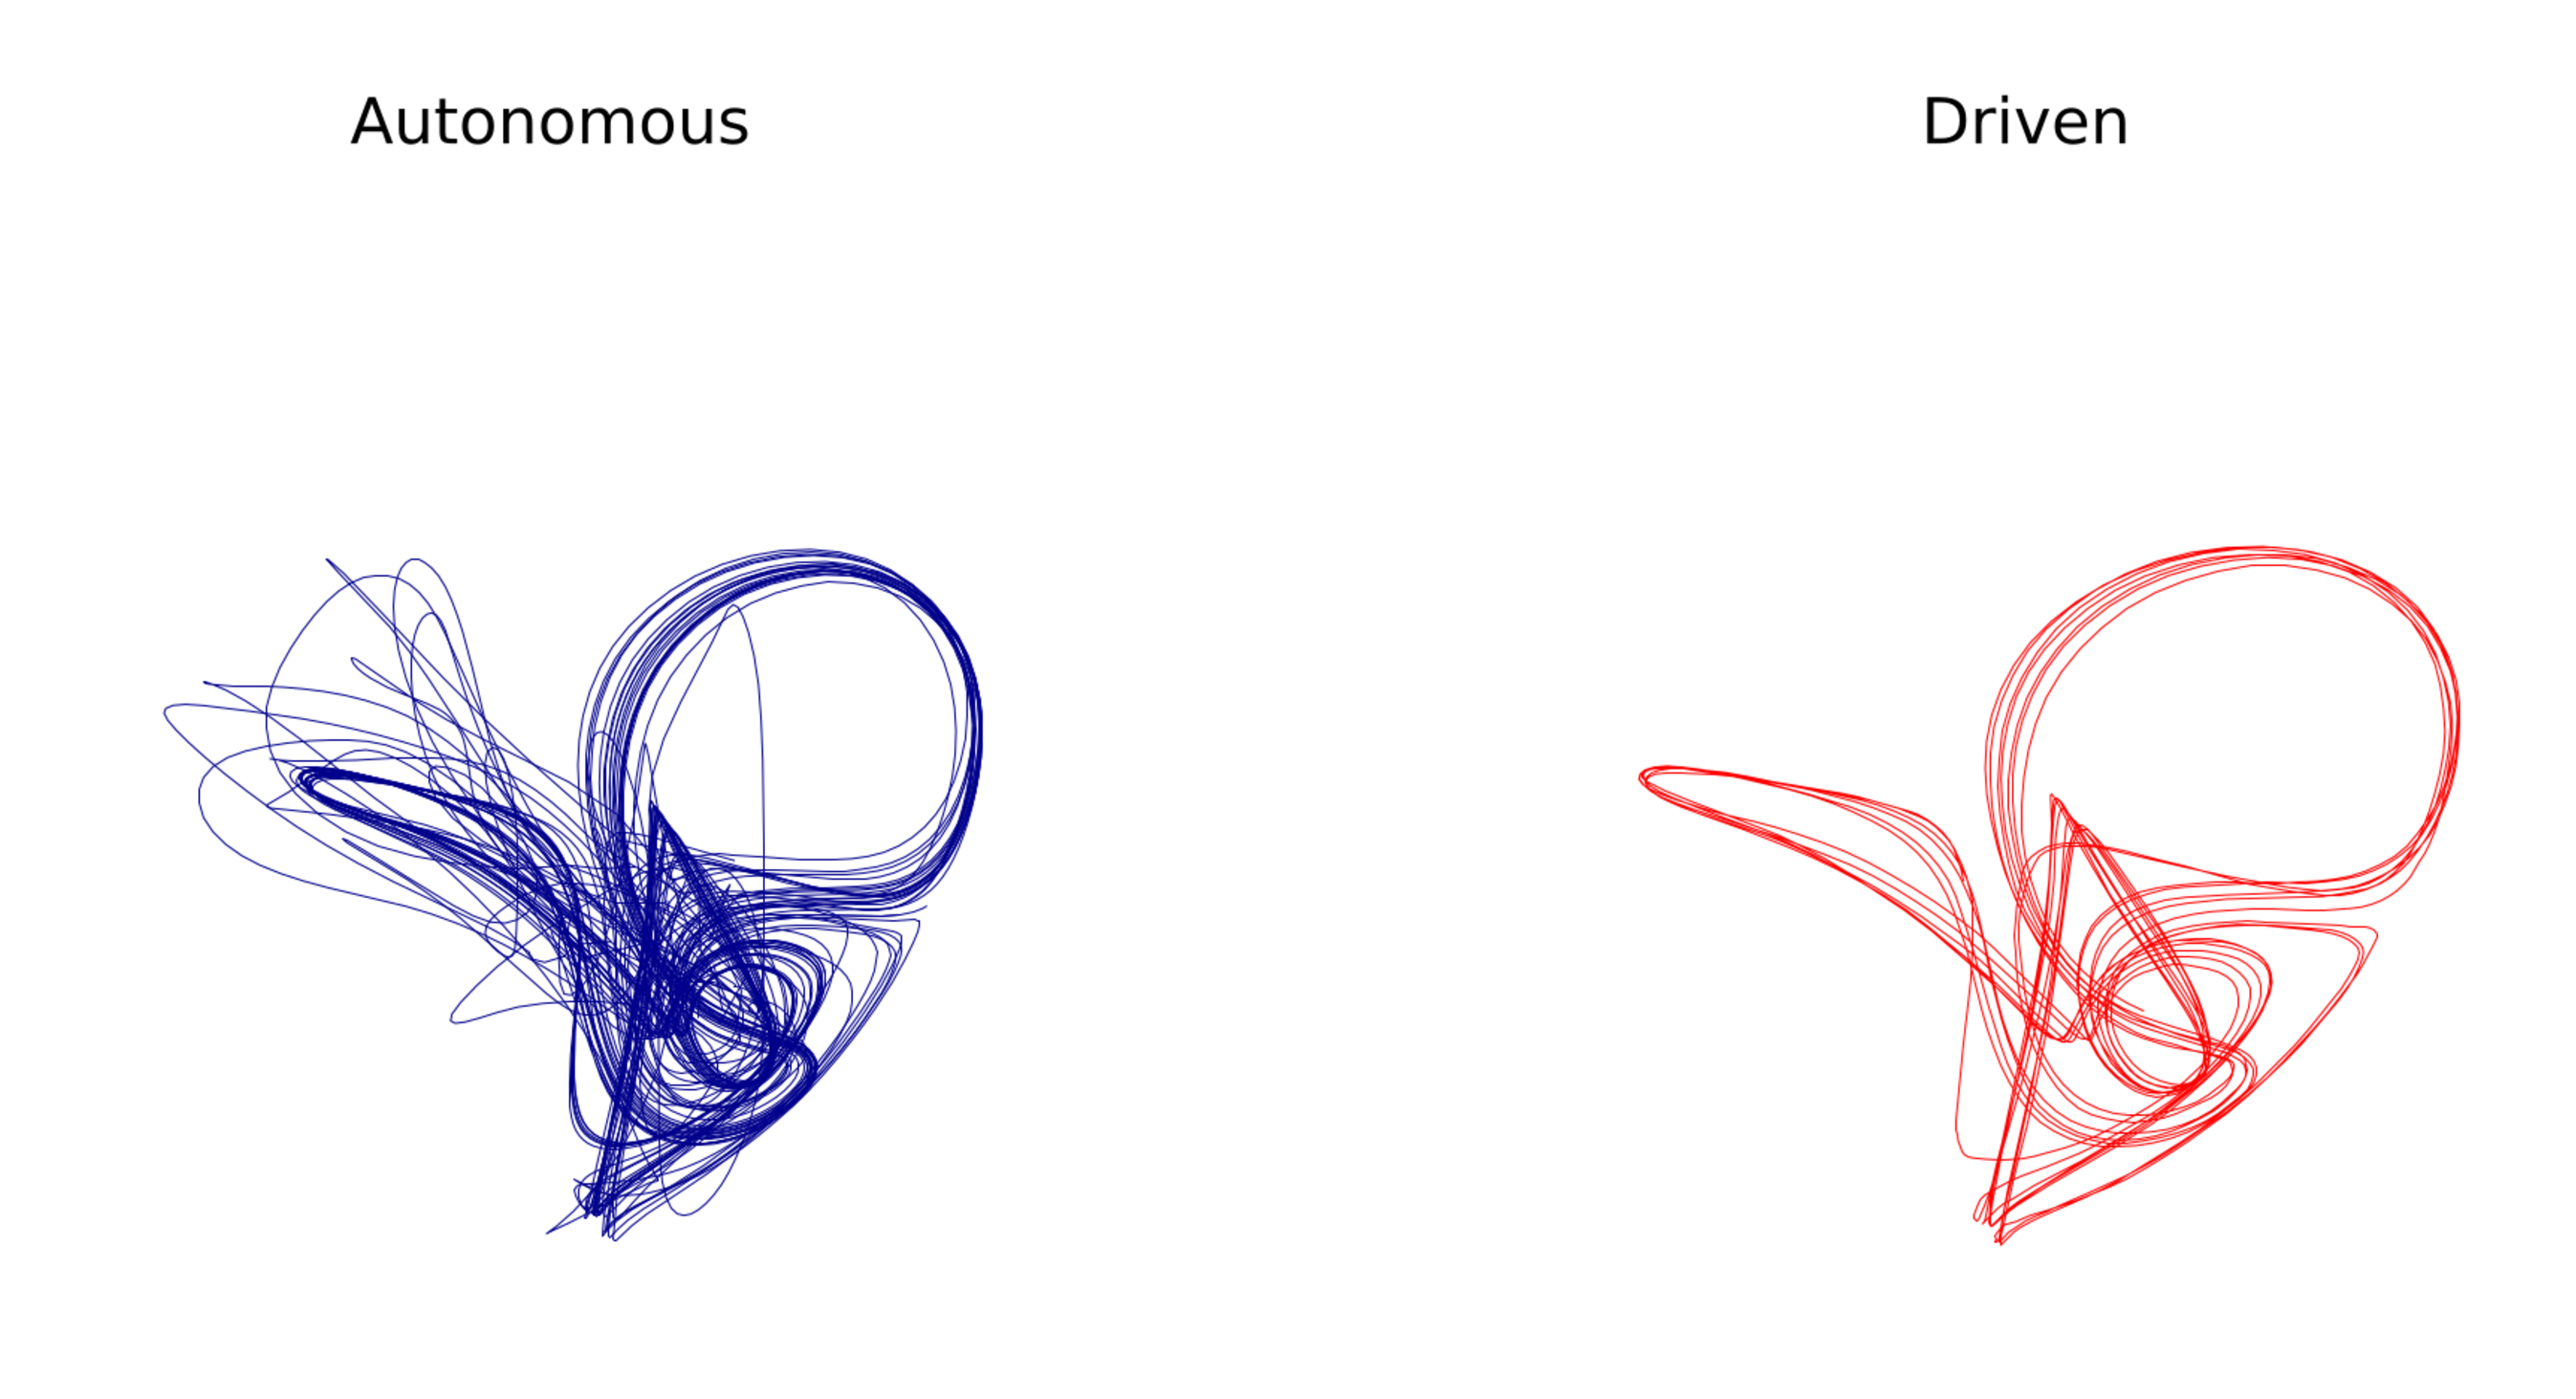
\includegraphics[scale=0.25]{_autovsdriven.eps}
  \centering
  \label{fig:learningFailure}
  \captionof{figure}{Illustrating empirically the importance of global dissipativity. Plotted below are the three principal components of randomly initiated points(blue) of a learnt version of $G_T$ versus the trajectory $(x_{n-1}, x_n)$(red) of driven states obtained from the Fractal Dream Attractor's data~\ref{Thomas_Attractor}). }
\end{figure}
\ednote{nice figure: Please rescale the figure and also you do not have to state that code was borrowed. So I have omitted that in the caption. Please put a caption to the figure and then cite in the text. }

Thirdly, whenever we learn a chaotic map on a set (here $Y_T$), as we had remarked in the disadvantages of Takens delay embedding a little noise would mean that the learnt system would accept arguments out of the set, so we will have a map $G_T^+$ acting on $Y_T^+$, and since $Y_T$ may not be an attractor of $G_T$ this could lead to errors. To circumvent this if the driven system with a saturation function is used, then we can ensure that there exists an attractor $A$ of the map that implements $G_T$ indirectly via $g$ containing $Y_T^+$. This prevents from large errors occuring since the dynamics is confined to $A$.  We refer to \cite{Supp} for details where this is referred to as the global dissipativity of $g$.   

In essence, global dissipativity prevents large numerical errors due to the noise in input data. If a system is not globally dissipative, neglibly small errors result could lead to major errors which thus induce predictions to fail utterly. If one learns $G_T$ directly, we are in danger of replicating the problems arising for Takens. 

%%%%%%%%%%%%%%%%%%%%%%%%%%%%%%%%%%%%%%%%%%%%%%%%%%%%%%%%%%%%%%%%


\chapter{Implementation} \label{ch5}
 
In this section we turn to the implementation of the function $G_T$ by discussing a method to learn the function $\Gamma$. We then indicate where this implementation differs from previous work done by (\cite{manjunath2021universal}) and empirically show that the SDD of $G_T$ are less functionally complex than $\Phi_{k, \theta}$ or $T$ by considering the Pearson correlation coefficient. 
Finally, we present and discuss some numerical results for a focus system of this project: the double pendulum. We also consider other chaotic attractors.

\section{Implementing $G_T$}
The map $G_T$ is implemented by applying the functions $\Gamma$, $g$ and the projection function $\pi_2$ in the relevant order as described by the equations~\ref{eqns_from_data}. To reach this point, one must first learn $\Gamma$.
After first normalising the data to ensure it lies within the interval $|x| < 1$ and has zero mean value, we continue by driving the system with external input through the function $g$.

From \eqref{eqn_driving} we know that $ g(u,x)=(1-a)x+a{\cdot}\tanh(Au+\alpha{a}Bx)$. Recall that $g$ is SI-invertible. Adopting the terminology of \cite{manjunath2021universal}, $A$ is called the “input matrix” and $B$ the “reservoir matrix”. 

We make use of a Recurrent Neural Network (RNN) in our implementation. RNN's are widely used in the literature for discrete-time processing and are considered to be discrete-time version of continuous dynamical systems modelling a network of neurons. (\textbf{Citation.})
A complete discussion of RNN's is outside the scope of this thesis, so we present only the details necessary to the current discussion. For information, (\textbf{Cite, Cite, Cite}) may be consulted. We implement our RNN in the \emph{Python} programming language and making use of the \emph{Scipy} library, alongside the \emph{Keras} package in the \emph{Tensorflow} library.

If the RNN we will be using in the next step has $N$ neurons, then $A$ and $B$ are each $N\times{N}$ matrices. Inputs $u_n$ of dimension $K < N$ are padded by zeroes to obtain an input of dimension $N$. As we do not need the entire left-infinite history of input, an arbitrary initialisation of the system with initial values followed by the driving of the system with the function $g$ means that the generated values will approach the actual solution’s elements in a uniform manner thanks to the UAP. \textbf{(Citation)}

Thirdly we prepare the network. Utilising a network $N$ neurons (the same value $N$ as in the dimensions of the matrices $A,B$). Training is done using the Adam Optimiser where the MSE loss function is optimised. The system is trained several times(in our case 4) with incrementally smaller learning rates on each run (0.001 and thereafter divided by 10 at each run). 
Additional parameters such as the number of network-layers, neurons per layer and training-length are presented case-by-case below.

We then reach the prediction step. Making use of $g$'s SI-invertibility and $g$ as defined in \eqref{eqn_driving}, we have the following expression for $u_n$ replicated from~\eqref{eqn_SI_RNN}.
\begin{equation*}
  u_n := A^{-1}\bigg(\overline{\tanh}^{^{-1}}\frac{1}{a}\Big(x_{n+1}-(1-a)x_n\Big) \bigg) - \alpha B x_n
\end{equation*}
    
The two model equations for learning from data (\eqref{eqns_from_data}) allows us to determine what the state $x_{n+1}$ at time $n+1$ will be. 
We specifically remind ourselves of \[x_{k+1}=\pi_2 \circ (\Gamma, \pi_2) \circ (\pi_2,g) (u_k,x_k)\]

\section{Changes in this project to previous work of~\cite{manjunath2021universal}}

To understand the first and most drastic\ednote{change word} change, we recall the the conjugacy in~\ref{fig:inverse_limsystem}:

\begin{equation*}
  %  \[ 
      \psset{arrows=->, arrowinset=0.25, linewidth=0.6pt, nodesep=3pt, labelsep=2pt, rowsep=0.7cm, colsep = 1.1cm, shortput =tablr}
      \everypsbox{\scriptstyle}
      \begin{psmatrix}
      \widehat{U}_T  && \widehat{U}_T \\
      Y_T && Y_T \\
      %%%
     %  \ncline{1,1}{1,2}^{\widehat{T}} \ncline{1,1}{2,1} <{h}
     %  \ncline{1,2}{2,2} > {H_2}
     %  \ncline{2,1}{2,2}^{G_T}
      \end{psmatrix}
    %  \]
  \end{equation*}
 
  We recall that $G_T$ is topologically conjugate to $\widehat{T}$, a result which we have already made use of.
  
  The authors of~\cite{manjunath2021universal} did not, however, consider the relationship between the inverse-limit space $\widehat{U}_T$ and the input $u_n=\theta(w_n)$ (where $\theta$ is our observable and $w_n$ the complete input), a concept we now explore.
  We may construct a delay-coordinate $v_n=[\theta(w_n), \theta(w_{n-1}), \ldots, \theta(w_{n-d})]^{T} = [u_n, u_{n-1}, \ldots, u_{n-d}]^T$
    to accordingly obtain a new dynamical system $(V,F)$ where $F$ is the map $F:v_n\mapsto{v_{n+1}}$. If $d$ is sufficiently large, we may apply Takens Embedding Theorem~\ref{Thm_Takens} to establish the existence of a topological conjugacy between the new system $(V,F)$ and the original system $(U,T)$.

  Using the same notation as before, we may construct a new conjugacy which now relates delay coordinates to one another.

  \begin{equation}\label{eqn_VFdelay}
    %  \[ 
        \psset{arrows=->, arrowinset=0.25, linewidth=0.6pt, nodesep=3pt, labelsep=2pt, rowsep=0.7cm, colsep = 1.1cm, shortput =tablr}
        \everypsbox{\scriptstyle}
        \begin{psmatrix}
        \widehat{V}_F  && \widehat{V}_F \\
        Y_F && Y_F \\
        %%%
       %  \ncline{1,1}{1,2}^{\widehat{F}} \ncline{1,1}{2,1} <{h}
       %  \ncline{1,2}{2,2} > {*}
       %  \ncline{2,1}{2,2}^{G_F}
        \end{psmatrix}
      %  \]
    \end{equation}

The existence of $\widehat{F}$ is guaranteed, but the map $v_{n}\mapsto{v_{n+1}}$ itself is unknown.
We may, however, make use of the SI-invertibility of the function $g(u_{n-1}, x_{n-1})=x_n$ to conclude that
$(x_{n-1}, x_{n})$ determines $u_{n-1}$ uniquely. 

Accordingly $(x_{n-2}, x_{n-1}, x_{n})$ determines $u_{n-2}$ and $u_{n-1}$ uniquely and generally $(x_{n-d}, \ldots , x_{n-1}, x_{n})$ determines $u_{n-d}, \ldots u_{n-2}$ and $u_{n-1}$ uniquely.

We therefore need not know what $\widehat{F}$ is, as we can determine $v_{n+1}={[u_n, u_{n-1}, \ldots, u_{n-d}]}^T$ indirectly by determining the value of $(x_{n-d}, \ldots , x_{n-1}, x_{n})$, a much more feasible task.

Accordingly we define the following abbreviations:
\begin{itemize}
  \item Delay Coordinates (DC): A vector composed by appending a fixed amount of previous values to the final value.
  \item Single-Delay Dynamics(SDD): Dynamics generated by 2-element delay-coordinate vectors of the form $(x_{n-1}, x_n)$ where only one previous value is used.
  \item Multi-Delay Dynamics(MDD): Dynamics generated by arbitrary-length delay-coordinate vectors of the form $(x_{n-d}, \ldots , x_{n-1}, x_{n})$. ($d$ must be sufficiently large, but is unknown. We vary this parameter in experimentation.)
\end{itemize}

Within this framework, the PCA-implementation of~\cite{manjunath2021universal} is then considered to fall underneath the of auspices of what we term \emph{Approximated Multi-Delay Dynamics(AMDD)}.

% We have now seen that one may comfortably switch between the use of SDD or MDD when $g$ has SI-invertibility. /ednote{This sentence needs to be improved.}

Naturally, one would immediately suppose that the MDD approach would increased computation time and resource use as the internal matrices and datasets generated during learning would grow with every increase in the delay-parameter $d$. 

In fact, preliminary results indicate the opposite due the observation that the implementation of MDD is inversely proportional to the the dimension of the network (i.e. the number of neurons in the RNN) and possibly also the number of epochs/batch size necessary to produce reliable predictions. 
This, in turn, actually speeds up the computation-time and provides results of similar accuracy. \ednote{I did not have enough time to explore this properly. I can only hazard guesses and promise future research work in this project. How should I best convey this? }

\textbf{Secondly}

Sparse Matrices:
\vspace{-8mm}
\begin{itemize}[noitemsep]
\item Well-conditioned: condition number close to 1
\item Scaled
\item Sparsity/density ratio
\end{itemize}

% Sparse matrix implementation. Slight improvement in some scenarios, but not fantastic. \ednote{M: Did it not help you a great deal with the DP forecasting? B: Sparse matrices tended to be finicky. In some cases they helped whereas in others they actually worsened the solution somewhat. There's some tuning to be done in terms of condition number, scaling and density}


\textbf{Third}

Density of matrices A/B(i.e. number of non-zero entries in each matrix) (separate from sparse matrix implementation)

\section{Numerical simulations}
In this section we showcase numerical results pertaining to 3 attractors that were simulated using the methodology described in the previous chapters. We first consider a simple physical system.
\subsection{Double Pendulum}

The Double Pendulum consists of two pendulums fastened to one another such that the system moves as a whole. The first (or higher pendulum) is attached to a fixed point while the second is attached to the endpoint of the first. (See below)
This system is a classical example of a system exhibiting chaos. \textbf{(Citation.)} Consider again~\ref{fig:dp_sdic}.
The system has four variables: angle and angular velocity of each pendulum rod. An ideal system is assumed where the rods are massless and no friction in the pivots are considered.

\begin{figure}[ht]
  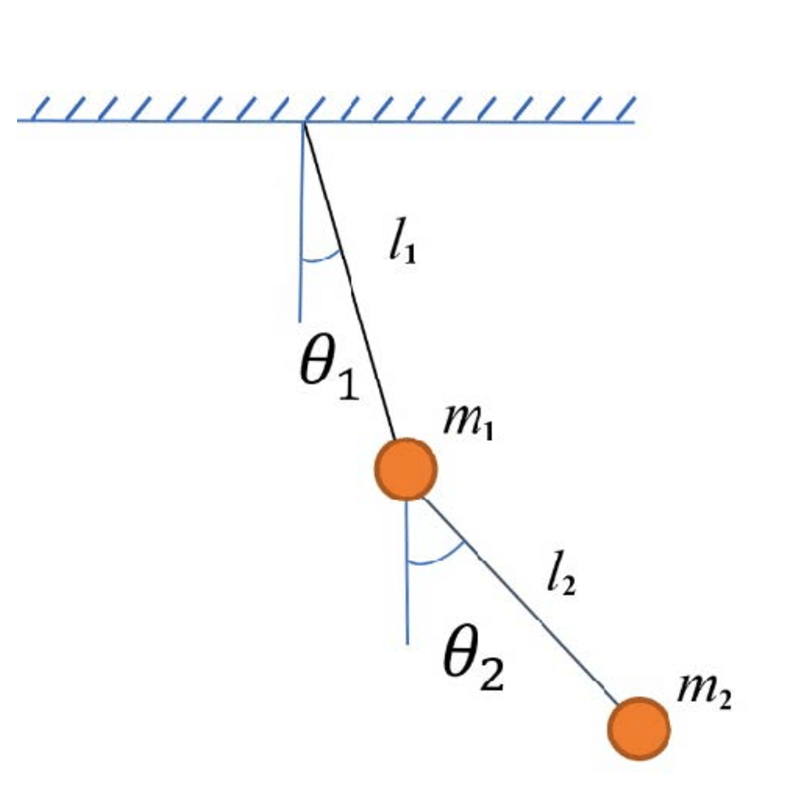
\includegraphics[scale=0.35]{_dp_setup.eps}
  \centering
  \captionof{figure}{Pictorial representation of the setup of a DP. Image taken from~\cite{DPSetup}}
  \label{fig:dp_setup}
\end{figure}

The scalar equations of motion are derived using Newtonian physics and can be found in~\cite{DPFormulas}. The second-order system is converted to a first-order ODE and solved using the Runge-Kutta numerical method.  Noise-free, undamped DP data-sets were generated and utilised in this project due to the requirement that the map $T$ be surjective. We discuss the case of a DP exhibiting energy-loss (i.e. where the map $T$ is not surjective) below.

\textbf{Data originating from a non-surjective map.}

The importance of the requirement that data originates from a surjective map is observed learning failure of a map describing a damped DP.
Due to the assumption, the program discounted any possibility of energy-loss and we consider the example below. 

\begin{figure}[ht]
  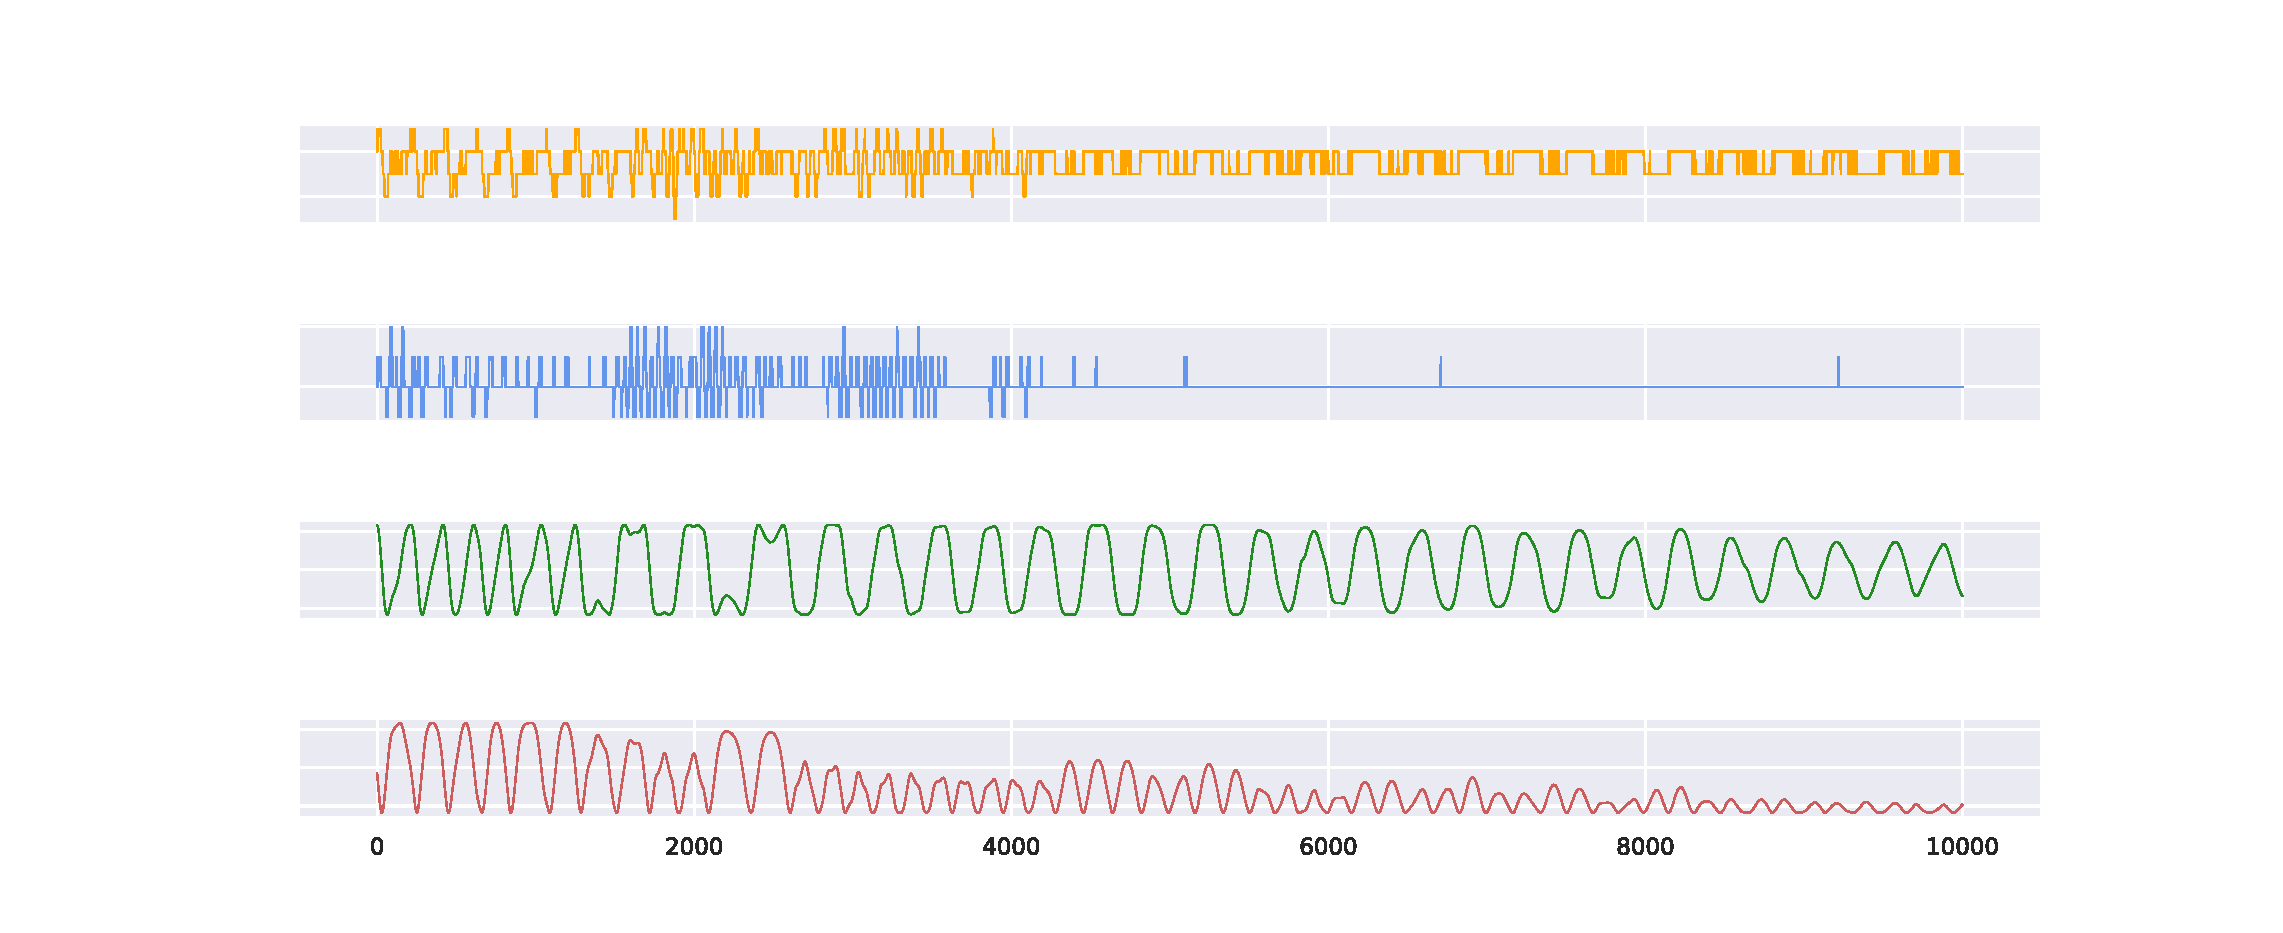
\includegraphics[scale=0.4]{_dp_dying.eps}
  \centering
\caption{The map generating data for a damped pendulum is not surjective. Data obtained from chaotic double pendulum dataset generated by~\cite{asseman2018learning}}
\label{fig:damped_pendulum}
\end{figure}

Despite feeding data that originated from a DP with dying occilations into the system, a map was instead learnt which continued to oscillate in a chaotic, but conservative manner.

\begin{figure}[ht]
  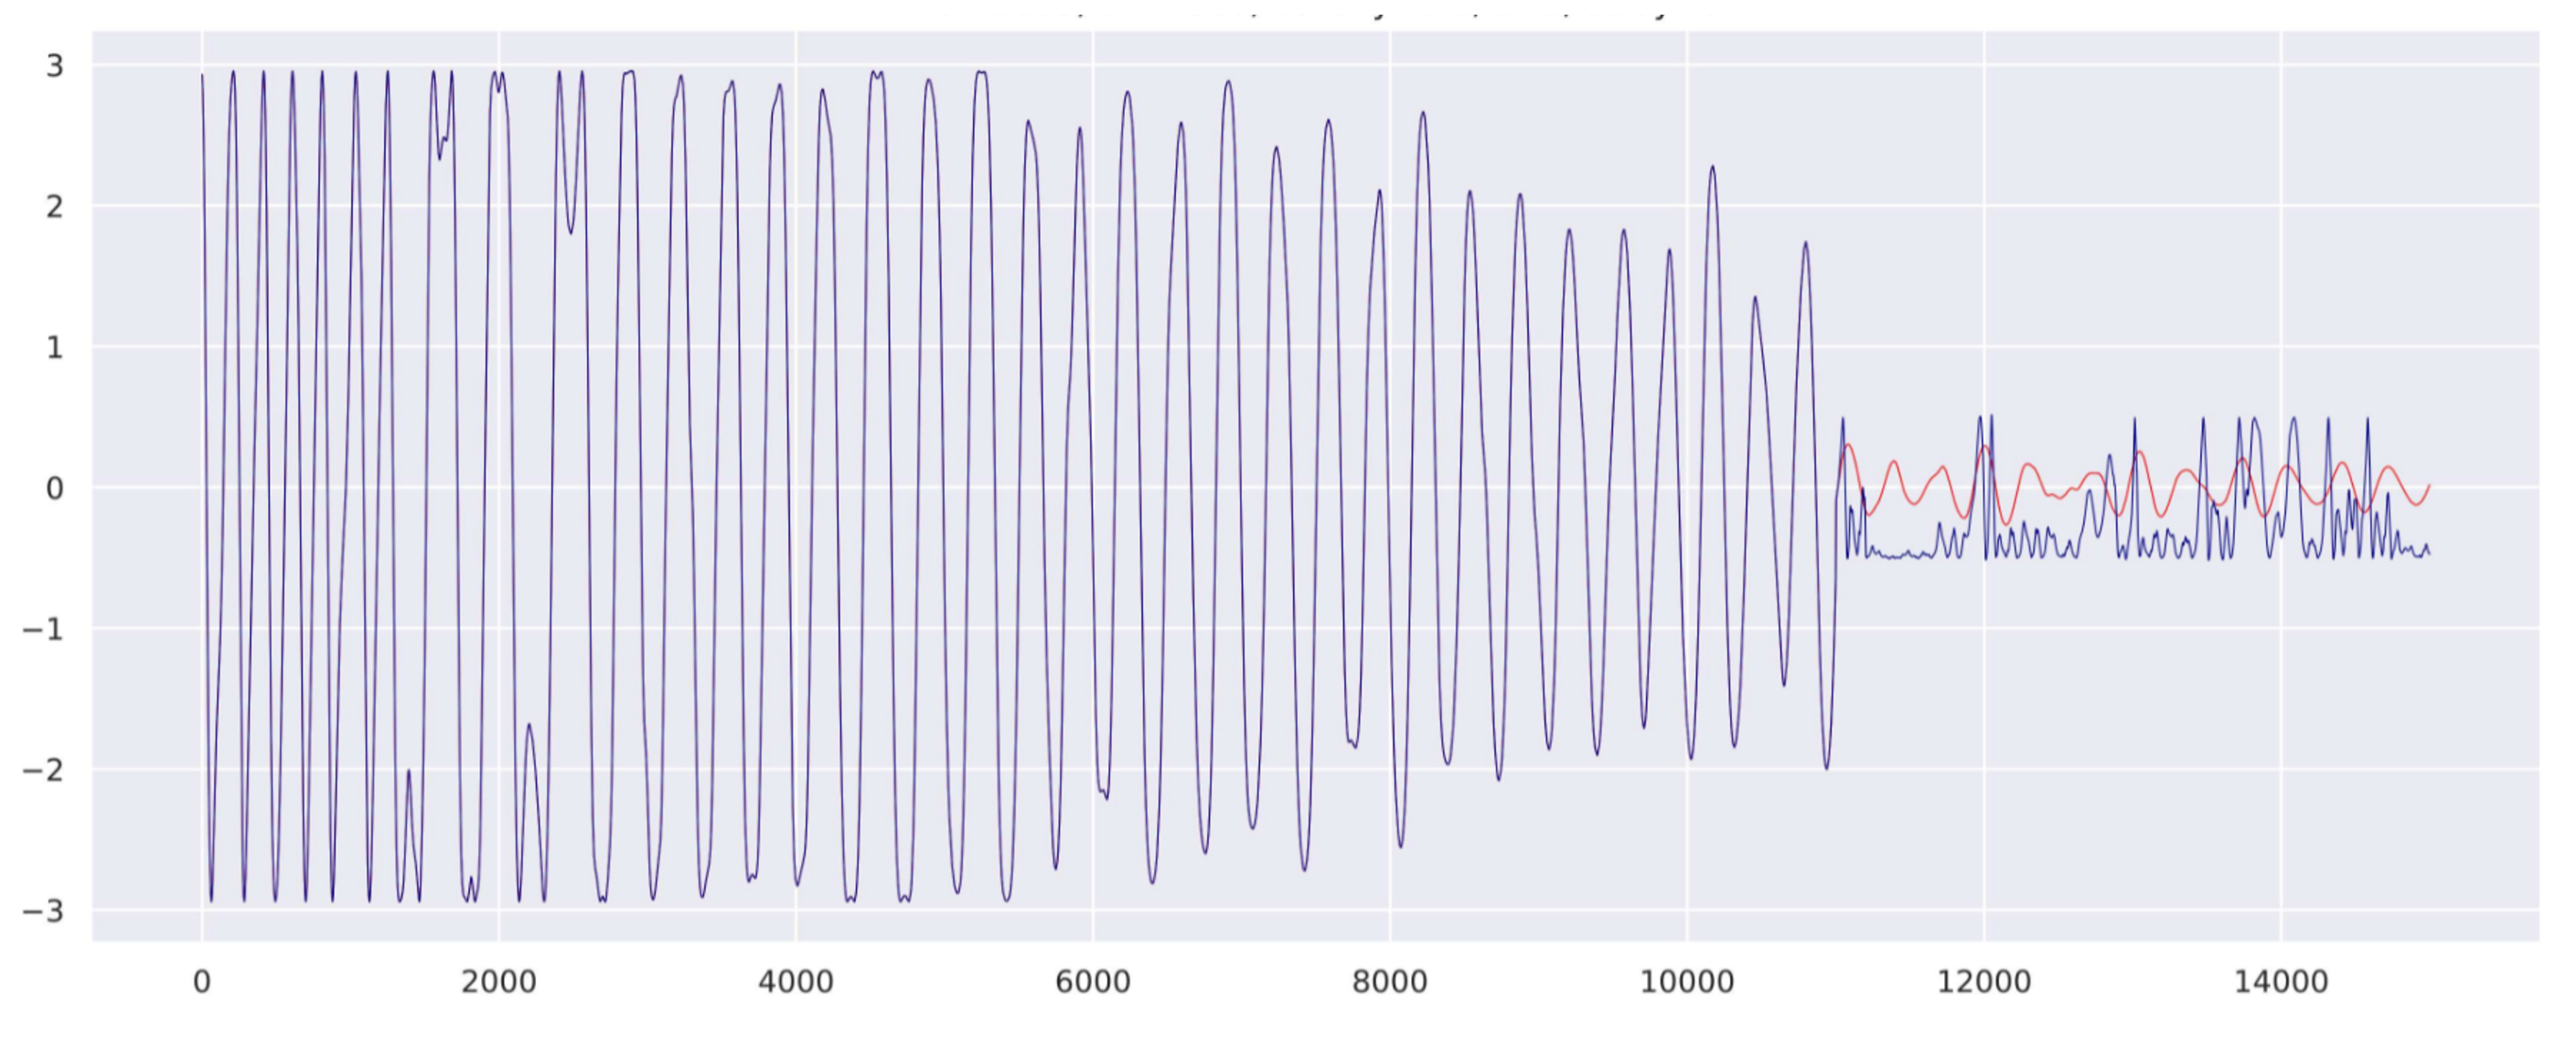
\includegraphics[scale=0.4]{_dpfail_nonsurj.eps}
  \centering
\caption{Failure to learn a map which is not surjective.}
\label{fig:dp_notsurjective}
\end{figure}



Having spent ample time to discuss the challenges, we now change tone so as to satisfy the optimist.
We present successful run for DP-data to repdict the future movement of the pendulum.

The system was driven for 15500 steps, of which the first 500 were immediately discarded to simulate the network 'forgetting'. The driving function $g$ had input and reservoir matrices were implemented as sparse matrices filled to 20\%. Parameter-values of $\alpha=0.99$ and $a=0.5$ were used.
The remaining 15000 datapoints were used to train a network with 128 neurons. 
The network was initialised to contain 16 hidden layers each with a layer dimension of 64, activated with the tanh activation function.
Training was accomplished using 256 epochs with batch sizes 128 and a delay of 1. 

% Trainlen:15000; Predlen: 1000; Discard: 500; Dimension:128 neurons; $\alpha=0.99$; $a=0.5$. Hidden Layers: 16. Layer dimension: 64. Epochs:256. Batch Size: 128. Delay(for MDD): 8. Density of Sparse Matrices: 0.2. $d=1$

\begin{figure}[ht]
  \centering
  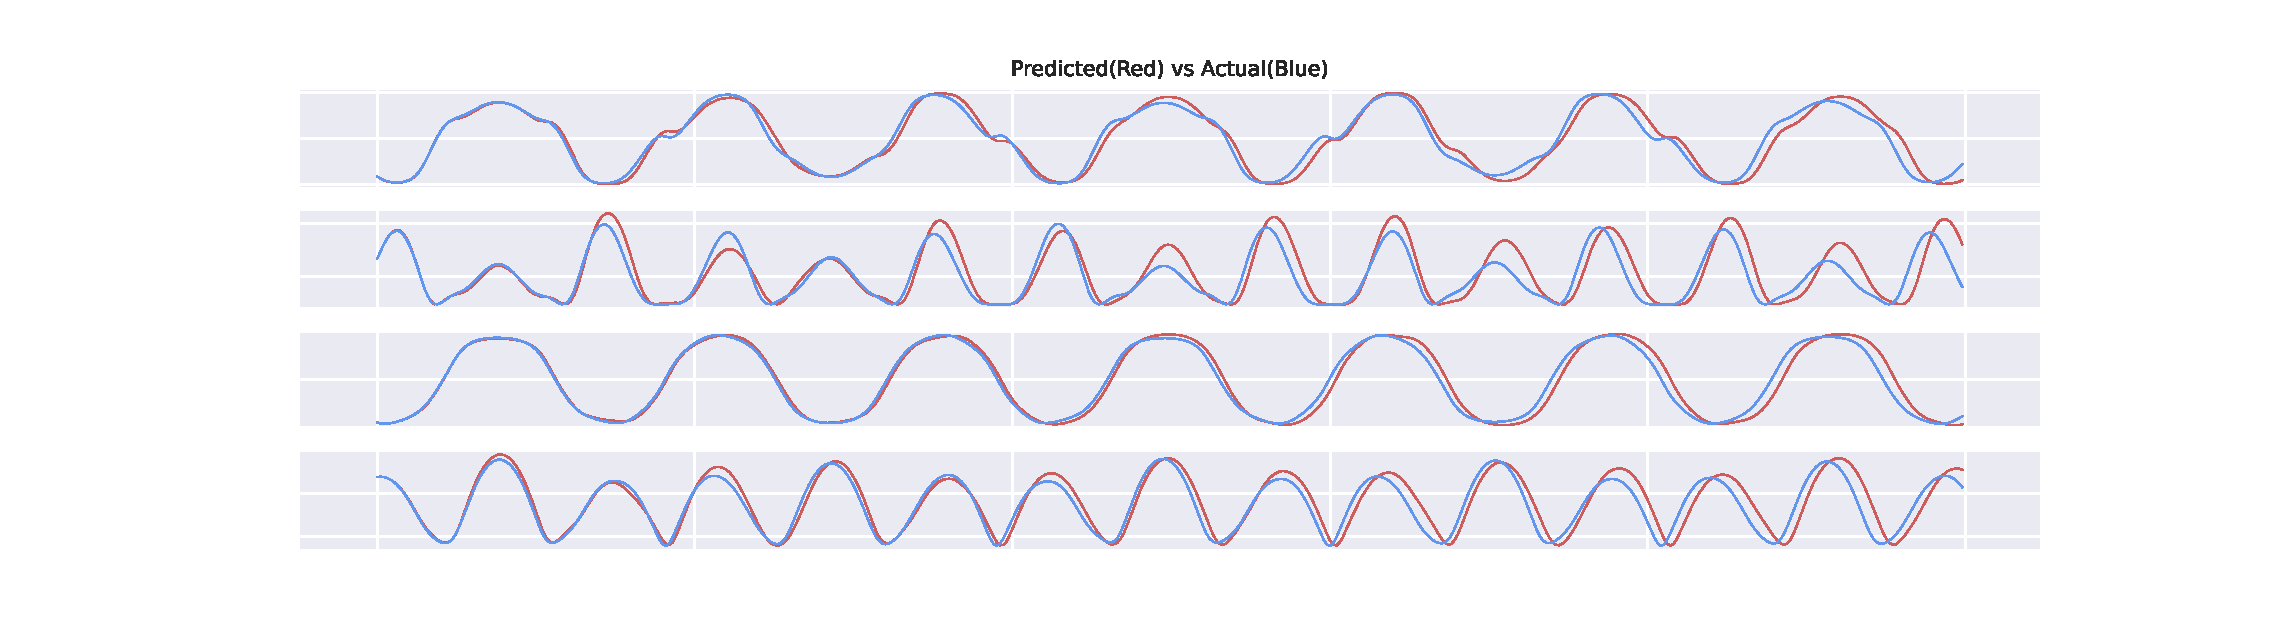
\includegraphics[width=0.8\linewidth]{_DP_Fig-2F2023.eps} 
  \captionof*{figure}{Predicted(red) and actual(blue) trajectories of the $x$- and $y$-coordinates of each of the pendulum heads.} 
% \end{figure}
% \begin{figure}[ht]
%   \centering
  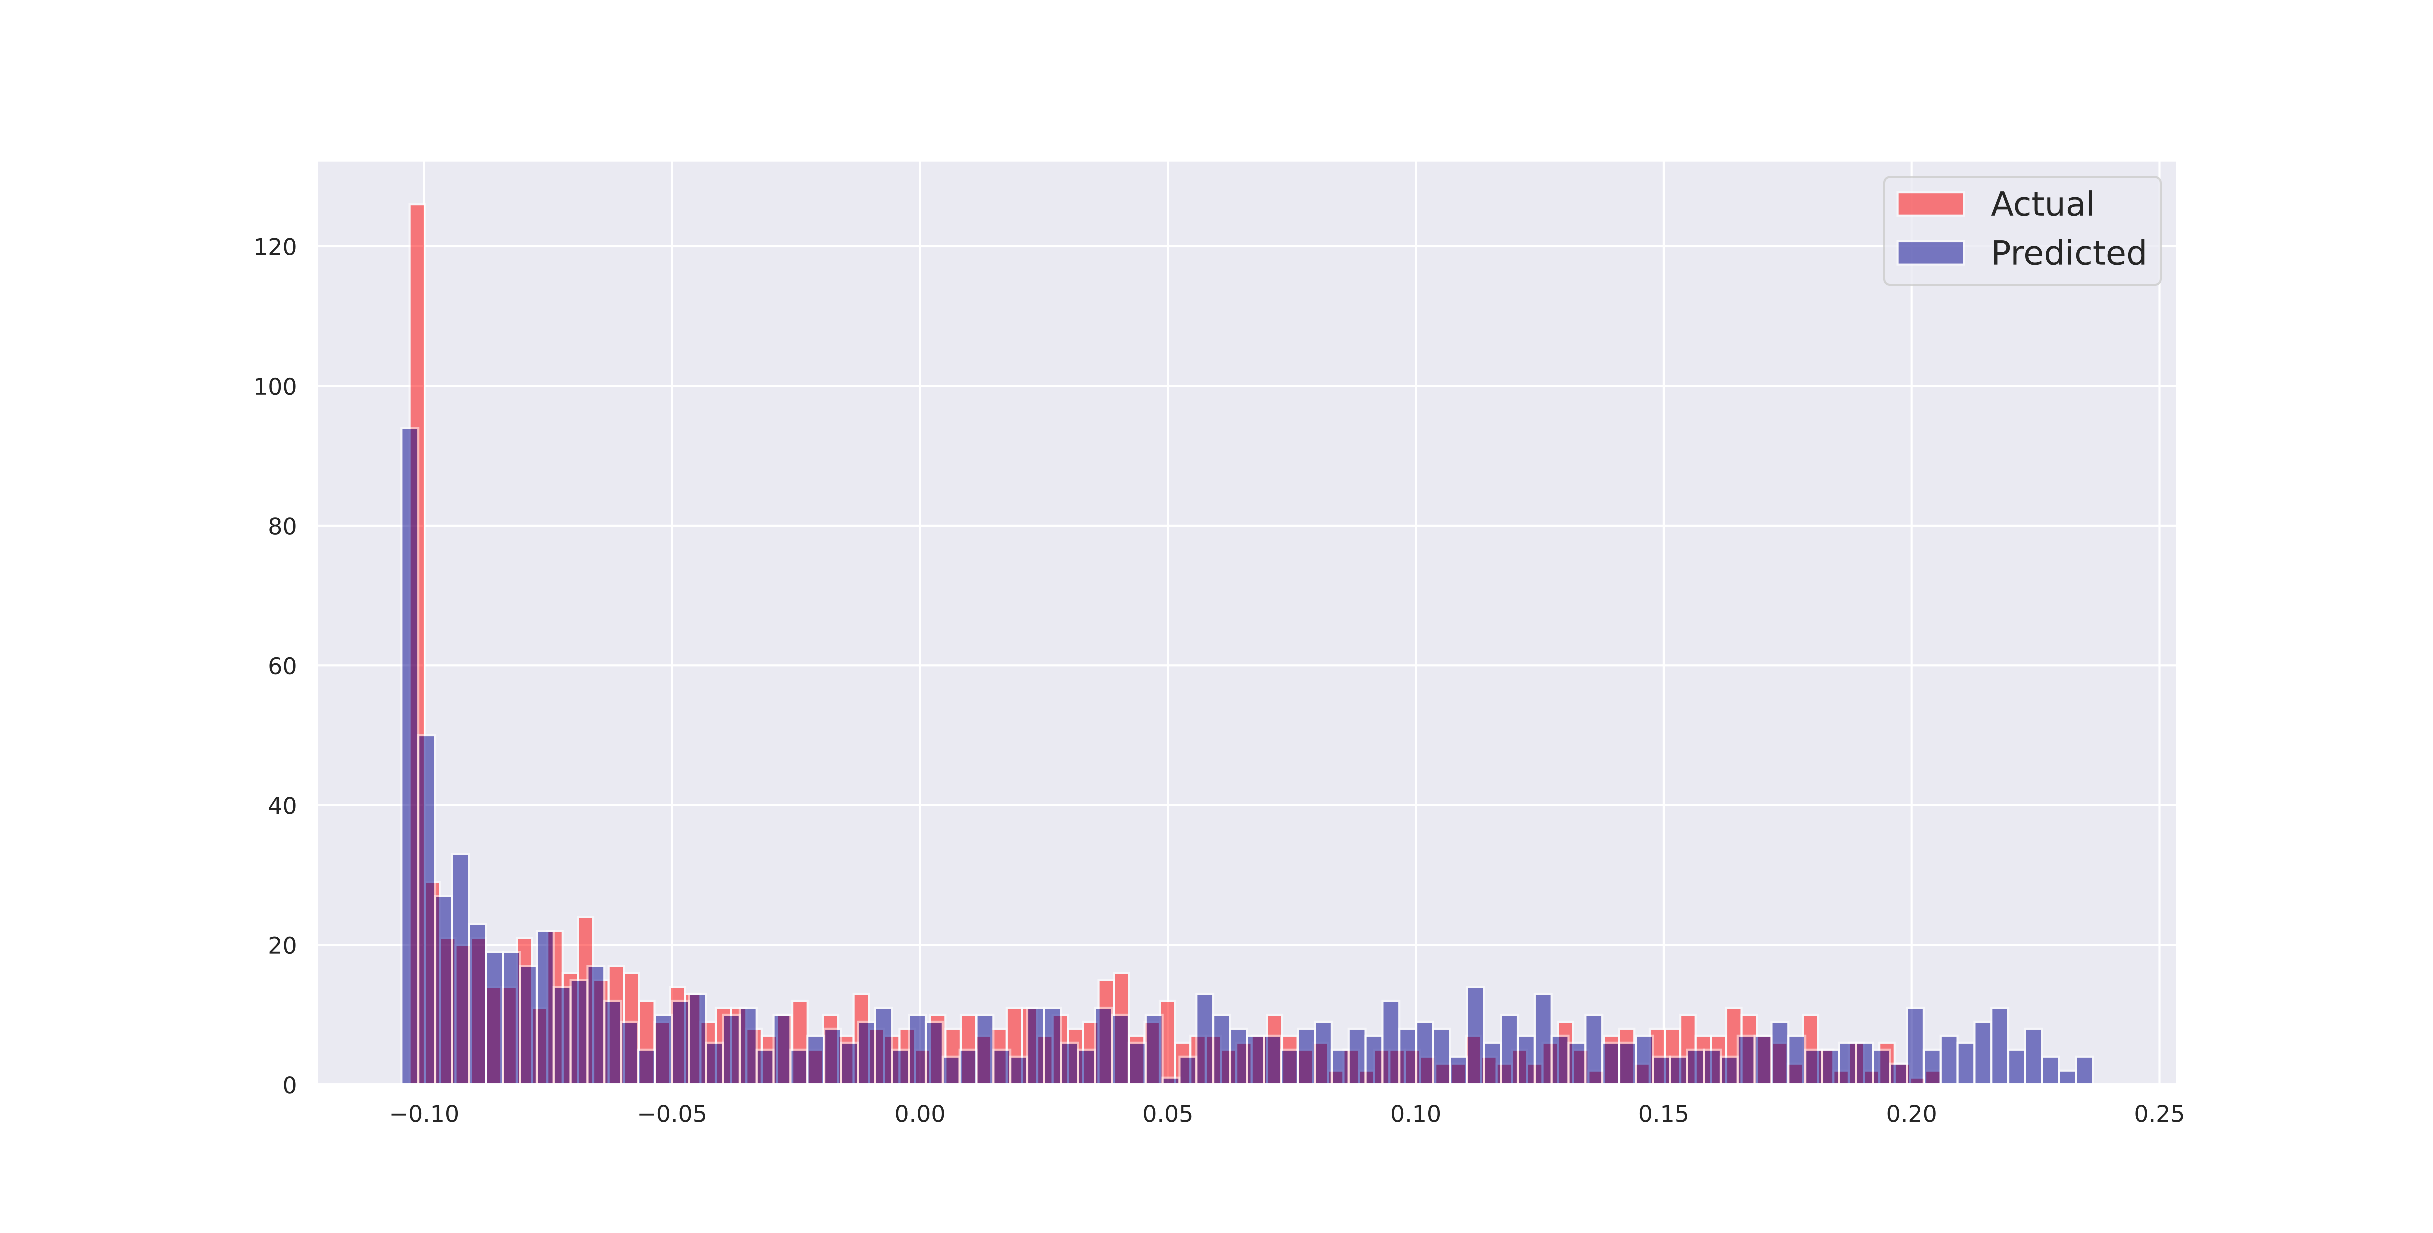
\includegraphics[width=0.8\linewidth]{_DP_Fig-2B2023.eps}
  \captionof*{figure}{Densities of predicted and actual values of x-coordinate of first pendulum head. }
  % \end{figure}
  % \begin{figure}[ht]
  %   \centering 
  \includegraphics[width=0.8\linewidth]{_DP_Fig-2D_5.eps}
    \captionof*{figure}{Takens Delay Map with delay=5 to illustrate behaviour of predicted and actual values of double pendulum data.}
    \label{fig:dp_predictions}
\end{figure}

\subsection{Additional Attractors: Clifford \& Thomas}
We follow the methodology presented in \cite{manjunath2021universal} but opt to consider attractors different from the Lorenz system and H\'enon map in this project.

\subsubsection{Thomas' Cyclically Symmetric Strange Attractor}\label{Thomas_Attractor}
Thomas' Cyclically Symmetric Strange Attractor, a 3D attractor proposed in 1999 by Ren\'e Thomas in \cite{ThomasAttractor}, is described by a set of three equations which is distinctly reminiscent of the Lorenz system, another deterministic three-equation model exhibiting chaotic behaviour.It has a single parameter $\beta$ and has been shown to transition to chaotic behavious when $\beta<0.208186$~\cite{Thomas_BetaParameter}.
\begin{eqnarray}\label{eqns_thomas}
  x_{n+1} = \sin(y_n) - \beta{x_n} \\
  y_{n+1} = \sin(z_n) - \beta{y_n} \\
  z_{n+1} = \sin(x_n) - \beta{z_n}
\end{eqnarray}

The behaviour of the system with a $\beta$-parameter value of 0.1056 was simulated by scaling it to fit inside the interval $[-1,1]$. Two cases were considered: noise-free and perturbed. Noise was generated from a normal distribution with mean 0 and standard deviation 0.05, which translates approximately to *dB.
 A sequence of 3000 observations in both the clear and noisy data-sets respectively were fed into the system with 300 entries discarded to simulate the network's loss of memory. The next 9000 steps were predicted and compared with true data.

\begin{figure}[ht]
  \centering
  \minipage{0.5\linewidth}
    \centering
    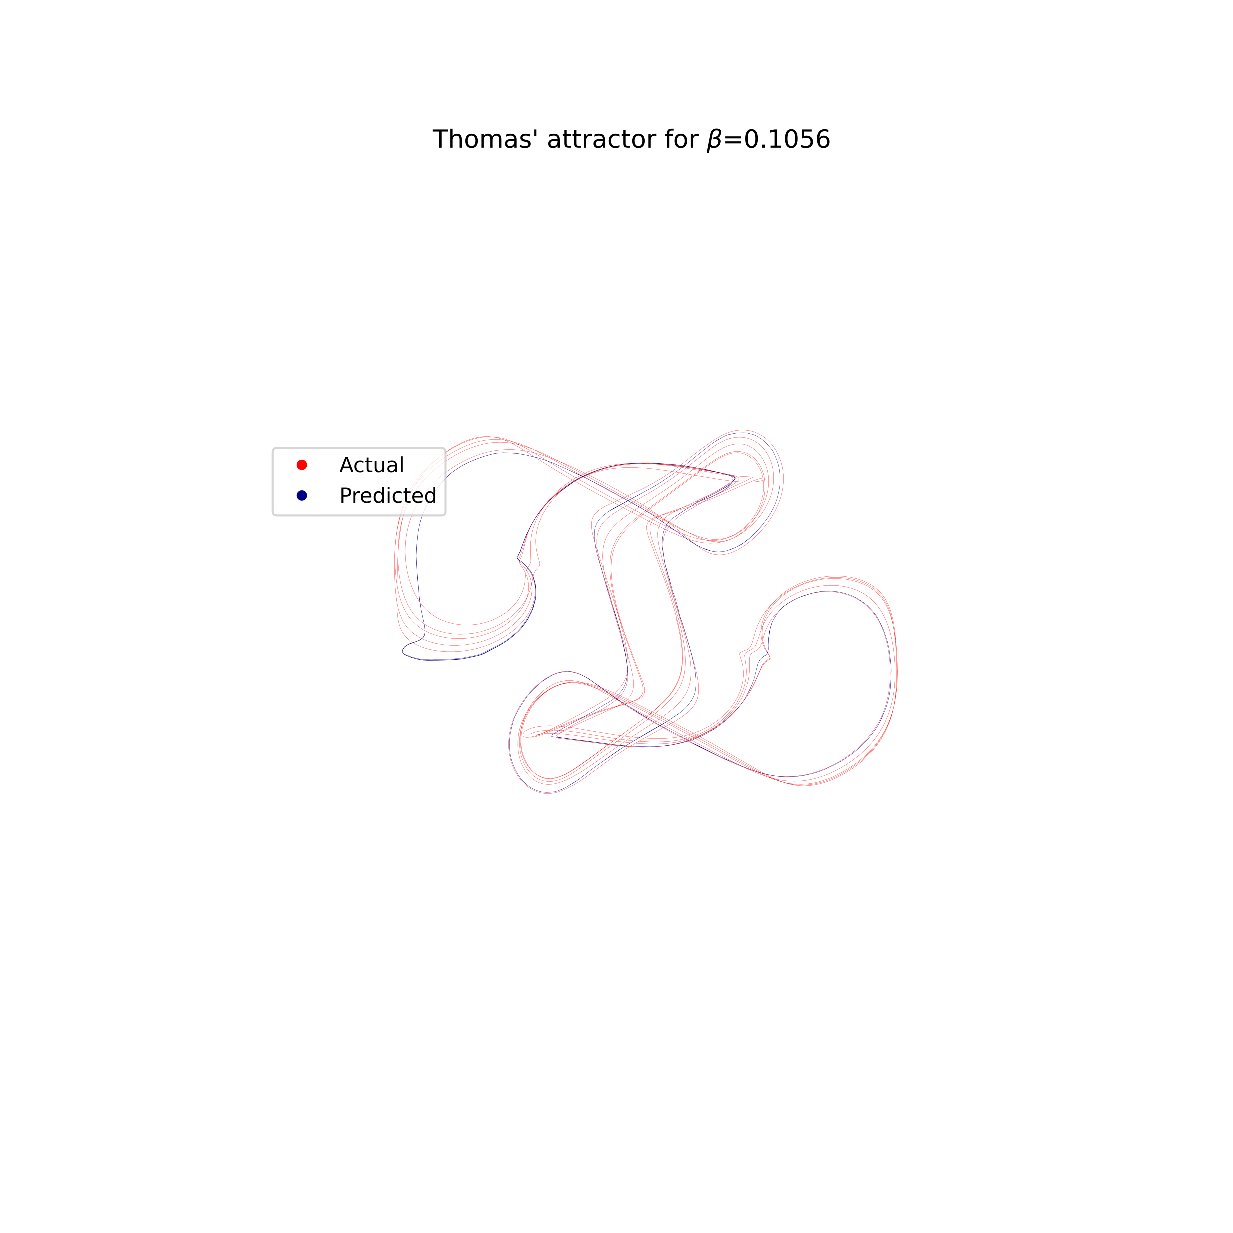
\includegraphics[width=\linewidth]{_Thomas_nonoise.eps}
    \caption*{True and predicted trajectories in the absence of noise.}
  \endminipage\hfill
  \minipage{0.5\linewidth}
    \centering
    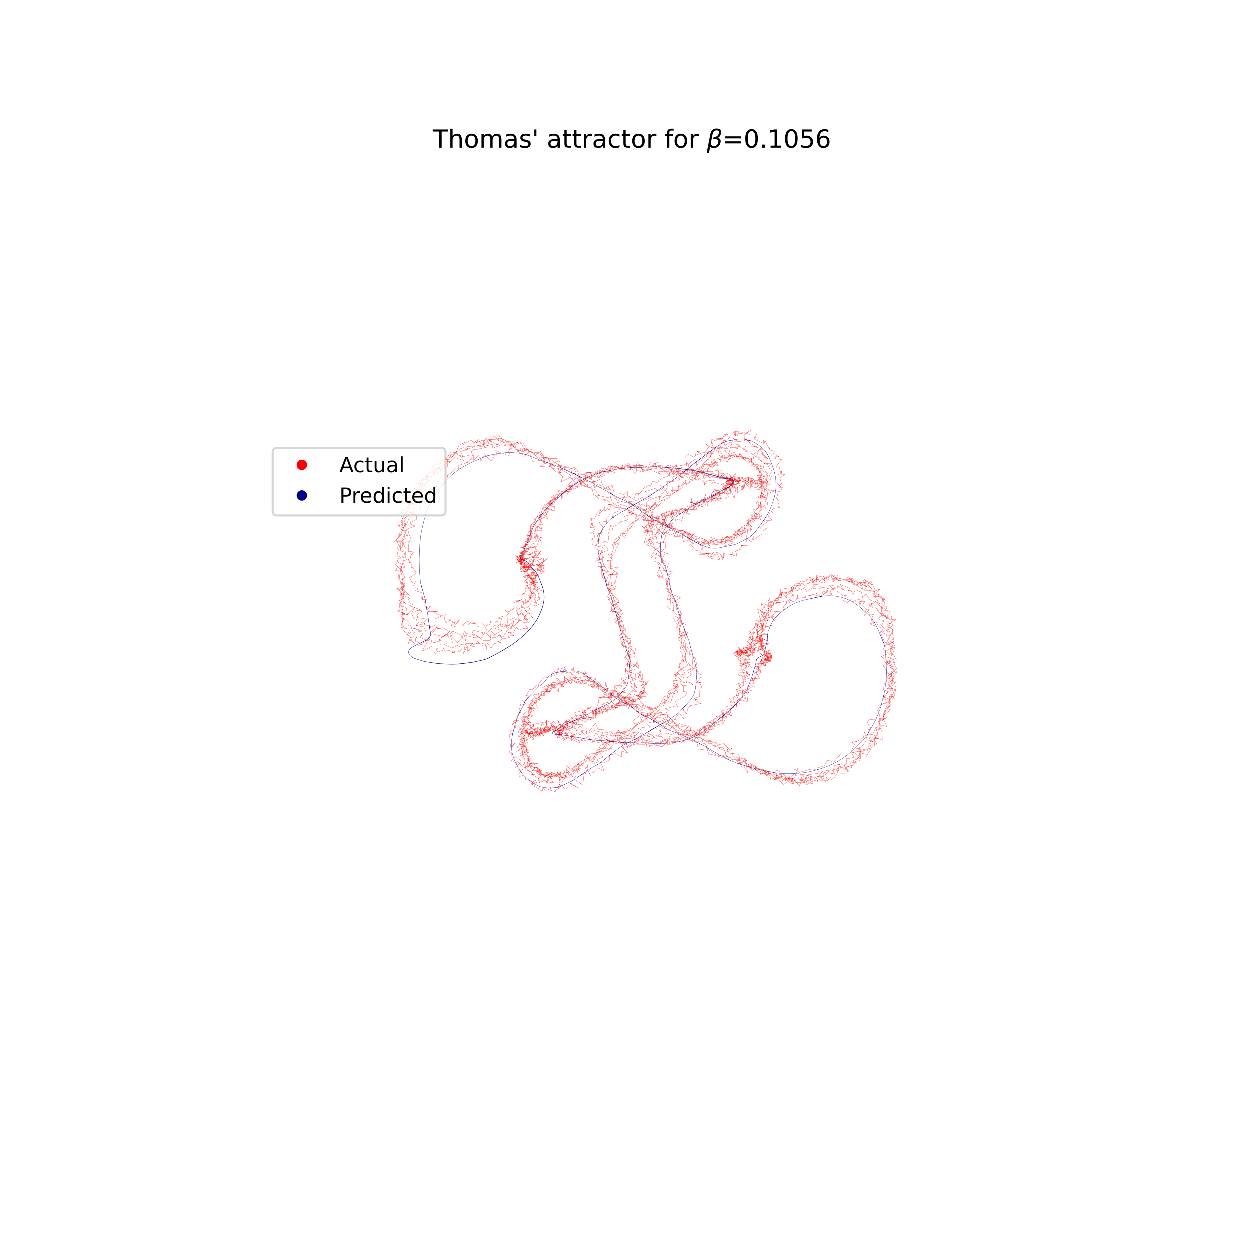
\includegraphics[width=\linewidth]{_ThomasNoisy.eps}
    \caption*{True and predicted trajectories for noise added.}
  \endminipage
\end{figure}

The RNN was initialised as follows: the dimension of the network is set equal to 500 neurons and 12 hidden layers of dimension 64 each were initialised. Training is realised through 150 epochs of batch sizes of 128 each; the map is learnt via the Adam Optimiser using finer and finer learning rates (0.001 and then divided by 10 at every iteration).

\begin{figure}[ht]
  \centering
  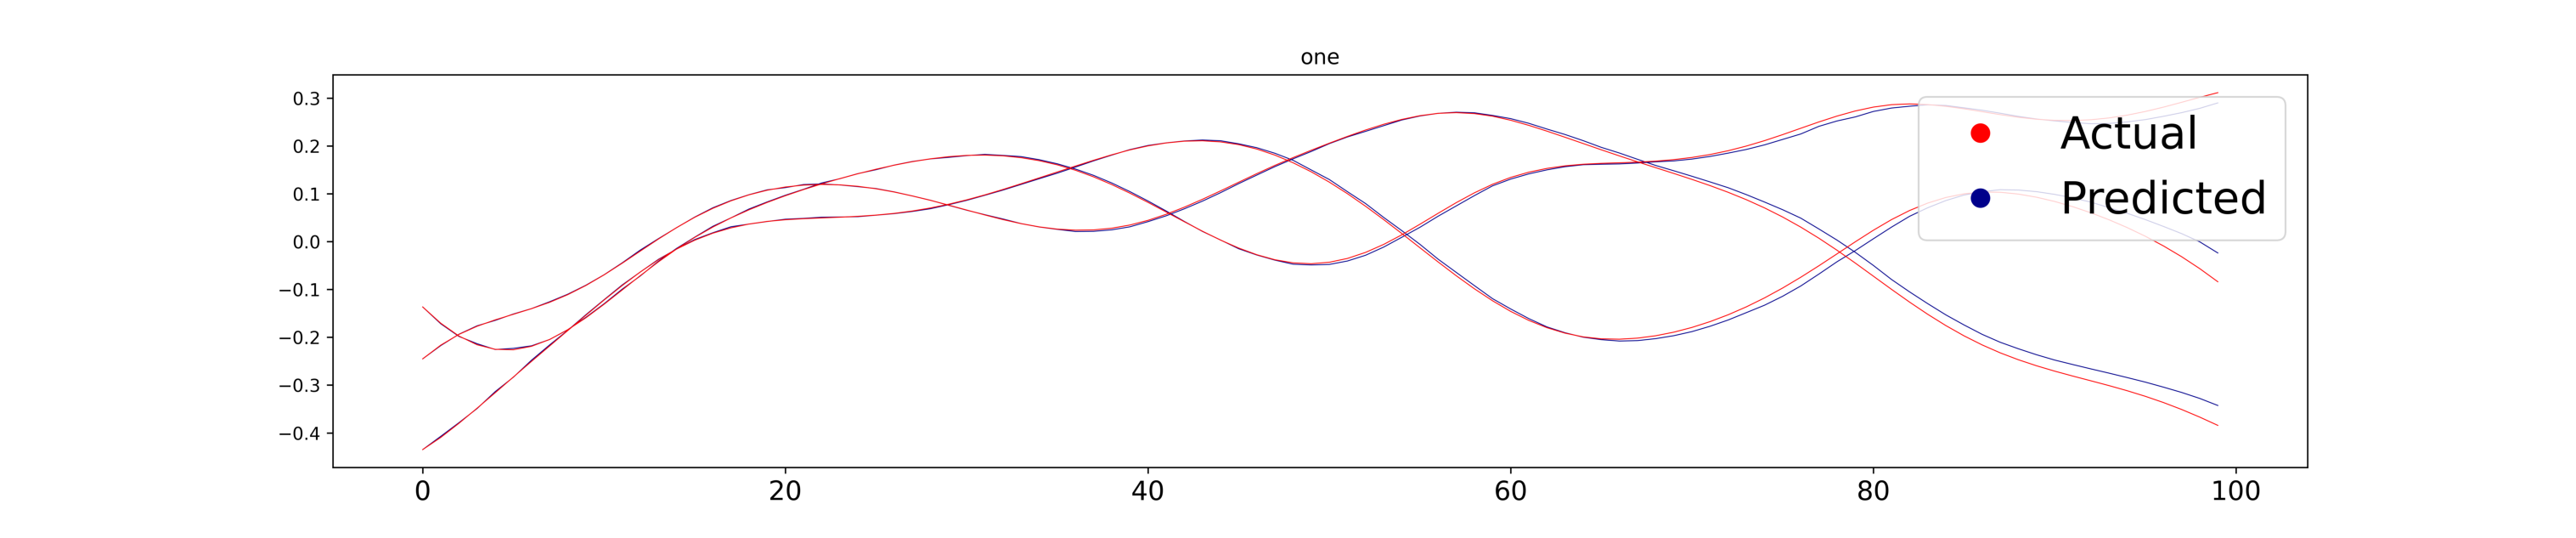
\includegraphics[scale=0.35]{_Thomas_1.eps}\caption*{Predicted trajectories for the attractor demonstrate empirically the ability to predict the evolution of the trajectory for the next ~100 timesteps}
  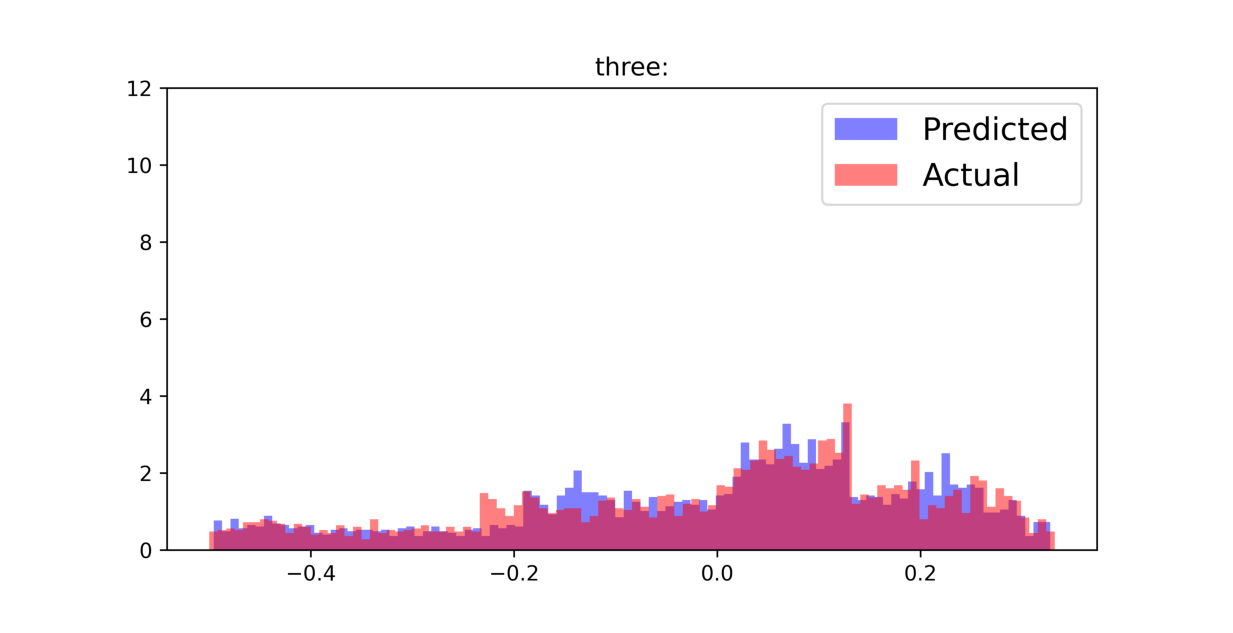
\includegraphics[scale=0.5]{_Thomas_3.eps}\caption*{Represented here the learnt (blue) and actual (red) densities of the first coordinate of the dataset.}
\end{figure}


\subsubsection{Fractal Dream Attractor}

Another 2-equation discrete-time map named the Fractal Dream Attractor, or more commonly known as the Pickover Map (first discovered by Clifford A. Pickover and discussed in his fascinating book "Chaos in Wonderland"\cite{PickoverChaos}), was also considered.
\begin{eqnarray}\label{eqns_clifford}
  {x_{n+1}=\sin(ay_n) + c\cos(ax_n)} \\
  {y_{n+1}=\sin(bx_n)+d\cos(by_n)}
\end{eqnarray}

\begin{figure}[ht]
  \centering
  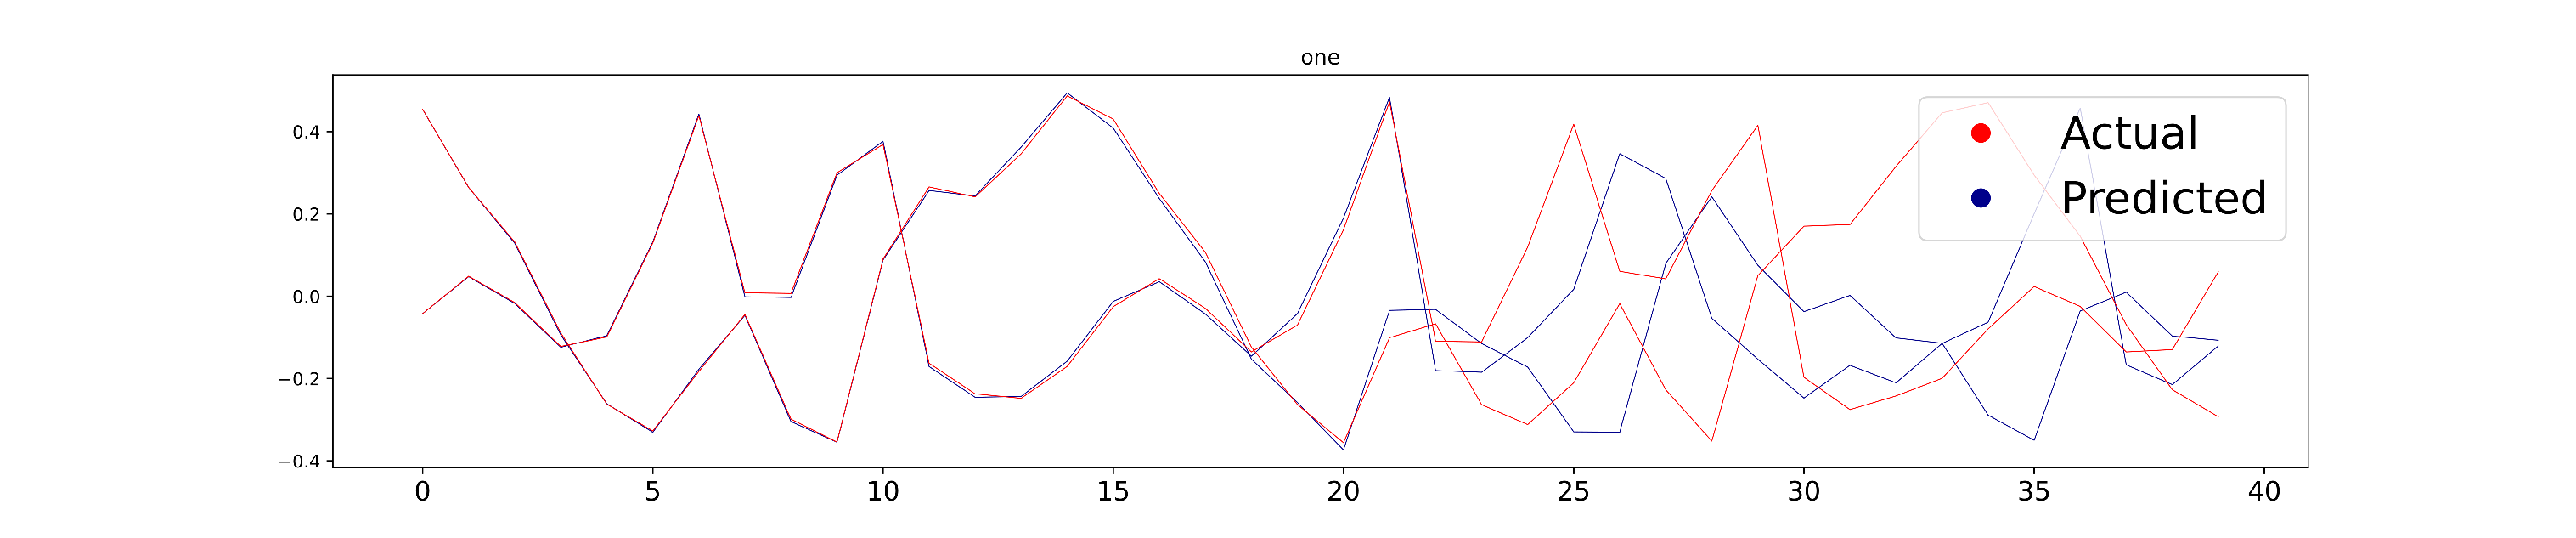
\includegraphics[width=1.0\textwidth,left]{Clifford_1.eps}
  \caption*{These graphs were constructed by predicting the Clifford system 15000 steps into the future and in so doing illustrating the long-term consistency and accuracy of the learnt system. As perceived here, we are able to lock on to the trajectory of the Clifford map almost exactly for the first 25 steps.}
  \minipage{0.5\textwidth}
      \centering
      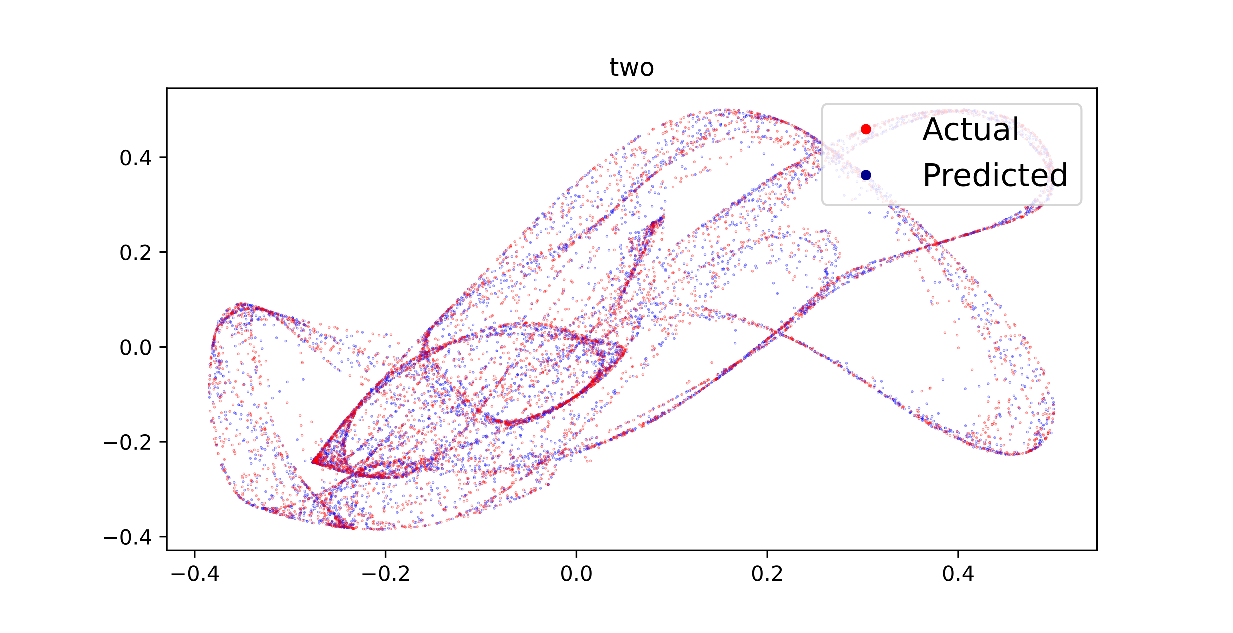
\includegraphics[width=\linewidth]{Clifford_2.eps}
  \endminipage\hfill
  \minipage{0.5\textwidth}
    \centering
    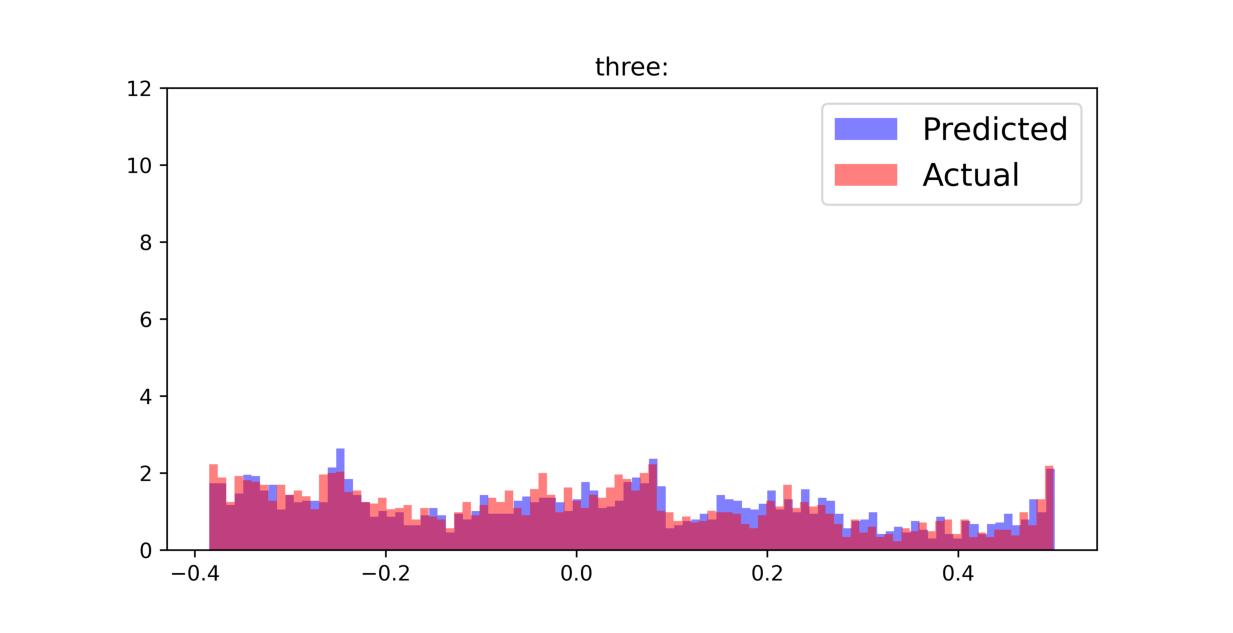
\includegraphics[width=\linewidth]{Clifford_3.eps}
  \endminipage
  \caption{The bottom row, left, shows a plot of the true attractor(red) and the predicted values(blue). Bottom row, right, shows the distribution of the first coordinate of the learnt system (blue) and the actual Clifford system (red). }
  \label{fig:Clifford}
\end{figure}

\ednote{B: Expand more.}

\section{Generalized Pearson Correlation}\ednote{B: Alter heading.}

% Besides being able to learn the action of the Koopman operator exactly, our setup has other advantages over selecting or optimizing the choice of observables as in the Extended Dynamic Mode Decomposition (EDMD) algorithm (e.g., [21, 22]). We can alter the functional complexity of G T by changing the number of observables or equivalently by altering the dimension of X – in the case of a RNN implementation of g, by simply changing the number of neurons in the network. Empirically, increasing the dimension of X is found to increase the linear relationship (or intuitively reduces the functional complexity of G T ) that is measured as a generalization of the Pearson correlation coefficient to random vectors (e.g., [44]) between (x_{n−1} , x_{n}) and G_T (x_{n−1} , x_n), and such numerical evidence is tabulated in [11, Table 1]. In contrast, expanding the set of observables while using EDMD to learn a map with a lower functional complexity is a highly involved task, not least because so much that one often does not know how to guess a new observable, as well as the fact that adding observables does not necessarily retain the invariance of the span of the observables.

% Empirical evidence shows that a linearity measure like a Pearson correlation coefficient points at reduced functional complexity while learning the dynamics in the state space of the driven system.

% Empirically (see Table ??), increasing the dimension of X is found to increase the linear relationship
% (or intuitively reduce the functional complexity of G T ) that is measured as a generalization of the Pearson correlation coefficient to random vectors (e.g., [?]) between (x n−1 , x n ) and G T (x n−1 , x n ). If Σ a and Σ b denotes the covariance matrices of the vectors (x n−1 , x n ) and G T (x n-1 , x n ) respectively, and if Σ ab denotes the covariance matrix between the vectors (x n-1 , x_n ) and G_T (x n-1 , x_n ), then the multidimensional 18correlation coefficient is computed by using the traces of these matrices: 
% \[\pho = \frac{tr(\sum_{ab})}{tr(\sqrt{\sum_{a}\sum_{b}})}\]

% This multidimensional correlation coefficient satisfies most of the well-known properties of the one-dimensional Pearson coefficient. In particular, ρ = ±1 if and only Y = AX + b for some invertible matrix A and vector b. Hence ρ, and in practice, the estimator ρ̂, can be used to measure the linear relationship between two random vectors of the same dimension and thus serves as an indicator of functional complexity.

% We remark that the estimation of such linear relationship in (see Table ??) obtained by sample correlations alone is justified whenever {u n } is a realization of an ergodic process since then when g has the USP, any solution {x n } is also a realization of an ergodic process [?]. In the ergodic input case the generalized Pearson correlation coefficient (between (x n−1 , x n ) and G T (x n−1 , x n )) is independent of n.

\ednote{B: Write Pearson Introduction. Could you give me some help here, Sir?}

\begin{center}
  \begin{table} 
      \scalebox{0.75}
      {\begin{tabular}{|c|c| c c |} 
          \hline
          Input & Dimension of $X$ & $u_n$ vs $u_{n+1}$ 
          & $\begin{bmatrix}
              x_{n-1}\\
              x_n
          \end{bmatrix}$ vs $\begin{bmatrix}
              x_n\\
              x_{n+1}
          \end{bmatrix}$ \\
          \hline
          
          % \hline
          % $(w_n)$ is the Lorenz states, sampled every 0.1 timestamps. & & &\\
          % \multirow{3}{*}{$u_n=\frac{1}{100}w_n$} & 10 &0.9311  & 0.9731\\
          %     & 100 &  & 0.9934\\
          %     & 1000 & & 0.9930\\
              
          % \multirow{3}{*}{$u_n=\frac{1}{10}(\sin(0.1w_{n,x})+\sin(0.1w_{n,y})+\sin(0.1w_{n,z}))$} 
          %     & 10 &0.8401  & 0.9392\\
          %     & 100 & & 0.9616\\
          %     & 1000 & & 0.9737\\
          % \hline
          
          \hline
          $(w_n)$ comes from the Thomas Attractor (for $\beta=0.1056$): & & & \\
          {$w_{n+1}= \begin{bmatrix} \sin(w_{n,y}) - \beta{w_{n,x}} \\
              u_y = \sin(w_{n,z}) - \beta{w_{n,y}} \\
          u_z = \sin(w_{n,x}) - \beta{w_{n,z}} \end{bmatrix}$} & & & \\
          \multirow{3}{*}{$u_n = w_n - \overline{w}$}
              & 10 & 0.99989 & 0.999886 \\
              & 100 & &  0.999913 \\
              & 1000 & & 0.999901 \\
          \hline
          
          \hline 
          $(w_n)$ comes from Noise-Added Thomas Attractor (for $\beta=0.1056$): & & & \\
          {$w_{n+1}= \begin{bmatrix} \sin(w_{n,y}) - \beta{w_{n,x}} \\
              u_y = \sin(w_{n,z}) - \beta{w_{n,y}} \\
          u_z = \sin(w_{n,x}) - \beta{w_{n,z}} \end{bmatrix}$} & & & \\
          \multirow{3}{*}{$u_n = w_n - \overline{w}$}
              & 10 & 0.9994 & 0.99985 \\
              & 100 & &  0.99991 \\
              & 1000 & & 0.999895\\
          \hline
          
          \hline
          $(w_n)$ comes from the Thomas Attractor (for $\beta=0.208186$): & & & \\
          {$w_{n+1}= \begin{bmatrix} \sin(w_{n,y}) - \beta{w_{n,x}} \\
              u_y = \sin(w_{n,z}) - \beta{w_{n,y}} \\
          u_z = \sin(w_{n,x}) - \beta{w_{n,z}} \end{bmatrix}$} & & & \\
          \multirow{3}{*}{$u_n = w_n - \overline{w}$}
              & 10 & 0.99982 & 0.99981\\
              & 100 & &  0.999851 \\
              & 1000 & & 0.99984 \\
          \hline
  
          \hline
          $(w_n)$ comes from the Clifford Attractor \\ (for $a = -1.7; b = 1.8; c = -1.9; d = -0.4$): & & & \\
        {$w_{n+1}= \begin{bmatrix} \sin(aw_{n,y}) + c\cos(aw_{n,x}) \\ 
                                                                    \sin(bw_{n,x})+d\cos(bw_{n,y}) \end{bmatrix}$} & & & \\
          \multirow{3}{*}{$u_n = w_n-\overline{w}$}
              & 10 & -0.21713 & 0.78719 \\
              & 100 & &  0.8334 \\
              & 1000 & & 0.84854 \\
          \hline  
          % \hline 
          % $(w_n)$ comes from the Logistic map: & & & \\
          % {$ w_{n+1}  = 4w_n(1-w_n)$} & & & \\
          % \multirow{3}{*}{$u_n = w_n - 0.5$} 
          %     & 10 &-0.0314  & 0.5577\\
          %     & 100 &  & 0.7150\\
          %     & 1000 & & 0.7826\\
          % \hline
          % \hline
          % $(w_n)$ comes from the Svensson Attractor \\ (for $a = -1.7; b = 1.8; c = -1.9; d = -0.4$): & & & \\
          % {$w_{n+1}= \begin{bmatrix} d\sin(aw_{n,x}) - \sin(bw_{n,y}) \\ 
          %                                                             c\cos(aw_{n,x})+\cos(bw_{n,y}) \end{bmatrix}$} & & & \\
          %   \multirow{3}{*}{$u_n = w_n-\overline{w}$}
          %       & 10 & -0.2243 & 0.49698 \\
          %       & 100 & &  0.63310 \\
          %       & 1000 & & 0.71151 \\
          % \hline
          \hline
          $(w_n)$ comes from the DP \\ (for ): & & & \\
          \multirow{3}{*}{$u_n = w_n-\overline{w}$}
                & 10 & 0.99141 & 0.98916\\
                & 100 & &  0.99238 \\
                & 1000 & & 0.99278 \\
          \hline        
      \end{tabular}} %\ednote{http://paulbourke.net/fractals/peterdejong/}

      \caption{Following \cite{manjunath2021universal}, we determine the multidimensional correlation coefficients $\rho$ to evidence a general reduction in the functional complexity of the map $G_T$ emerging due to a RNN. Rows correspond to distinct dynamical systems considered in the experiments
      The second column corresponds to the amount of artificial neurons (the dimension of $X$) in the implemented RNN.
      The last two columns comprise numerical estimates of $\rho$ for the relevant vectors. The linear association between $u_n$ vs $T(u_{n})$, as well as the linear relationship $\begin{bmatrix}
              x_{n-1}\\
              x_n
          \end{bmatrix}$ vs $G_T \left( \begin{bmatrix}
              x_{n-1}\\
              x_n
          \end{bmatrix}\right)$ may be contrasted by the reader. 
          Finally, the RNN's dimension (from \eqref{Seq_RNN}) is provided to exhibiting that an increase in dimension of the driven system will 
          typically result in a map $G_T$ with less functional complexity.} 
          \label{Table_FC}
      \end{table}\label{tbl_attractorsPearson}
\end{center}
  

\chapter{Conclusion}\label{ch6}

% The driven states $(x_{n-1},x_n)$ hold the information of the left-infinite history of the input. Furthermore, there is some evidence that the inverse-limit space (not system) seems to distinguish two dynamical systems that are not topologically conjugate for a class of systems in the sense their inverse-limit spaces are not homeomorphic to each other.  So the relation $Y_T$, which is homeomorphic to the inverse-limit system, may be unique to a class of systems. (The reference is a paper on Ingram’s Conjecture by Marcy Barge, Henk Bruin and Sonja Stimac.) Further investigation is needed.  \cite{budivsic2012applied, korda2020data}

As technology has advanced over the past century, humanity’s ability to record and manipulate rich, complex data in order to produce forecasts has profoundly increased. 
Collecting measurements from underlying artificial, natural, and physical systems through observables to realise a dynamical model with greater descriptive power is well-established in present-day science.

Core to the success of these techniques is the fact that dynamics discerned from the observed space can often be characterised by a mapping of much lower functional complexity when compared to the map describing the unknown underlying system. Takens theorem and the numerous generalizations thereof is one such method establishing (under some generic conditions) the learnability of a system produced by creating a delay-coordinate vector from a sufficiently large number of previous observations of a dynamical system. This system is topologically conjugate to the system from which the observed time-series was obtained.

A critical concern of this method is the requirement of full knowledge of the variables of the underlying state space that govern the complex dynamical system one is interested in. In real-world conditions this intelligence is seldom available and one must depend heavily on human expertise and insight. 

Each discrete-time state space model has at its core a driven dynamical system. In this project, it has been shown that an input originating from a compact space entailing exactly one solution (i.e., if the driven system has the USP) is equivalent to representing information without distortion, a concept which was formalised by establishing a causal mapping’s existence. The established results are general, implying that any driven dynamical system with specific properties can give rise to a causal mapping, and in so doing  providing an answer as to the success of arbitrary choices of driven systems in information processing applications in [4, 5].

In particular, we have a topological conjugacy (semi-conjugacy) between the data comprising the 11single-delay lag dynamics of a driven system’s and the underlying homeomorphic dynamical system. Finite-length input data is sufficient for forecasting as driven system states are influenced only in an almost negligibly small manner by the left-infinite segment of the past of the input beyond some arbitrarily large but finite time (a result which holds due to the universal semi-conjugacy of a driven system’s continuity)


Viewed through the lens reservoir computing approaches, we have also demonstrated that when single-delay dynamics are utilised, a learnable map in a reservoir computing network certainly exists. Moreover, such a driven system within a reservoir computing network enjoys certain proven qualities pertaining to the robustness w.r.t input- and parameter-perturbation. Accordingly, we are able to preserve the quality of a representation that would otherwise remain sensitive to various fluctuations, rendering the learning of the system’s dynamics wholly unpredictable. In addition, we obtain the robustness of the system against external noise, a phenomenon which is observed for the Fractal Dream Attractor.

Finally, we consider some physical systems to observe the methodology in practice and verify that we can indeed predict the future evolution of chaotic systems such as the double pendulum. Empirical evidence shows that a linearity measure like a Pearson correlation coefficient points at reduced functional complexity while learning the dynamics in the state space of the driven system


Considered with a philosophical-scientific lens, this project has aimed to establish a juncture between rationalism (the theory of nonautonomous dynamical systems) and empiricism (machine learning) to yield results profitable to the discipline of Applied Mathematics. This was done by showing that dynamics in an observed space can be established as topologically conjugate to the underlying system. As a result of the topological conjugacy, deep learning techniques are then subsequently applied to physically such equations from the data. In so doing, we acquire models of high fidelity that provide exceptional forecasting results on chaotic data that exhibit both statistical and topological consistency in the long run.


\end{document}